\documentclass[12pt,initial,twoside,maitrise]{dms}
\usepackage[utf8]{inputenc} %Obligatoires
%\usepackage[T1]{fontenc}    %
\usepackage[dvipsnames]{xcolor}
\usepackage[scaled]{beramono}
\usepackage{ocr}
\usepackage[T1]{fontenc}
\usepackage{array}
\usepackage{algorithmicx}
\usepackage{algorithm}
\usepackage{algpseudocode}
\usepackage{amsmath}

\usepackage{natbib}
\usepackage{hyperref}
\hypersetup{colorlinks,citecolor=green}

\usepackage{enumitem}
\usepackage{graphicx}

% Quotes
\usepackage{epigraph}
\beforeepigraphskip=-20pt
\afterepigraphskip=20pt
\renewcommand{\textflush}{flushepinormal}

% Trees
\usepackage{tikz}
\usepackage{tikz-qtree}

% Table Checks
\usepackage{booktabs}
\usepackage{pifont}
\usepackage{float}

\newcommand{\wmark}{\textcolor{orange}{\ding{45}}}
\newcommand{\cmark}{\textcolor{green!80!black}{\ding{51}}}
\newcommand{\xmark}{\textcolor{red}{\ding{55}}}

\newcommand{\welldone}[1]{\textcolor{green}{#1}}
\newcommand{\mediumwell}[1]{\textcolor{blue}{#1}}
\newcommand{\medium}[1]{\textcolor{cyan}{#1}}
\newcommand{\mediumrare}[1]{\textcolor{orange}{#1}}
\newcommand{\rare}[1]{\textcolor{red}{#1}}
\newcommand{\argmax}[1]{\underset{#1}{\operatorname{arg}\,\operatorname{max}}\;}
\newcommand{\argmin}[1]{\underset{#1}{\operatorname{arg}\,\operatorname{min}}\;}

% Table
\newcommand*\rot{\rotatebox{90}}

\usepackage{menukeys}
\usepackage[skins,breakable,listings]{tcolorbox}
% Code listings
\lstdefinelanguage{kotlin}{
    comment=[l]{//},
    commentstyle={\color{gray}\ttfamily},
    emph={delegate, filter, firstOrNull, forEach, it, lazy, mapNotNull, println, return@},
    emphstyle={\color{OrangeRed}},
    identifierstyle=\color{black},
    keywords={abstract, actual, as, as?, break, by, class, companion, continue, data, do, dynamic, else, enum, expect, false, final, for, fun, get, if, import, in, infix, interface, internal, is, null, object, open, operator, override, package, private, public, return, sealed, set, super, suspend, this, throw, true, try, typealias, val, var, vararg, when, where, while, tailrec},
    keywordstyle={\color{NavyBlue}\bfseries},
    morecomment=[s]{/*}{*/},
    morestring=[b]",
    morestring=[s]{"""*}{*"""},
    ndkeywords={@Deprecated, @JvmField, @JvmName, @JvmOverloads, @JvmStatic, @JvmSynthetic, Array, Byte, Double, Float, Int, Integer, Iterable, Long, Runnable, Short, String},
    ndkeywordstyle={\color{BurntOrange}\bfseries},
    sensitive=true,
    stringstyle={\color{ForestGreen}\ttfamily},
    literate={`}{{\char0}}1
}

\lstdefinelanguage{docker}{
    keywords={FROM, RUN, COPY, ADD, ENTRYPOINT, CMD,  ENV, ARG, WORKDIR, EXPOSE, LABEL, USER, VOLUME, STOPSIGNAL, ONBUILD, MAINTAINER},
    keywordstyle=\color{blue}\bfseries,
    identifierstyle=\color{black},
    sensitive=true,
    comment=[l]{\#},
    commentstyle=\color{purple}\ttfamily,
    stringstyle=\color{red}\ttfamily,
    morestring=[b]',
    morestring=[b]"
}

\lstdefinelanguage{BashPrompt}{%
    keywordstyle=\color{blue},
    basicstyle=\ttfamily,
    literate={\$}{{\bfseries\textcolor{blue}{\$}}}1
    {~}{{\bfseries\textcolor{blue}{\textasciitilde}}}1,
}

\lstdefinelanguage{DtsPrompt}{%
    keywordstyle=\color{blue},
    basicstyle=\ttfamily,
    literate={dt> }{{\bfseries\textcolor{blue}{dt> }}}1
}

\lstdefinelanguage{XML}{
    basicstyle=\ttfamily,
    morestring=[s][\color{black}]{"}{"},
    morestring=[s][\color{black}]{>}{<},
    stringstyle=\color{black},
    identifierstyle=\color{blue}\bfseries,
    moreidentifier={launch, node},
    keywordstyle=\color{brown},
    morekeywords={name, pkg, type, output},
}

\lstdefinelanguage{bnf}{
    basicstyle=\ttfamily,
    morestring=[s][\color{RoyalPurple}\bfseries]{"}{"},
    emphstyle={\color{ForestGreen}\bfseries},
    moreemph={TYPE, KEY, SEPARATOR, VALUE, COMMENT},
    identifierstyle=\color{blue}\bfseries,
    keywordstyle={\color{NavyBlue}\bfseries},
    morekeywords={property, recover_property, rosInterfaceFile},
    ndkeywords={getType, get Key, getValue, getName, setName, getNameIdentifier},
    ndkeywordstyle={\color{black}\itshape},
}

%% Adjustments

\lstdefinestyle{barelisting}{
    language=kotlin,
    basicstyle=\ttfamily\scriptsize,
    numberstyle=\footnotesize,
    backgroundcolor=\color{gray!10},
    frame=single,
    tabsize=2,
    rulecolor=\color{black!30},
    breaklines=true,
    inputencoding=utf8
}

\usepackage{lipsum}
\tcbuselibrary{listings,breakable}

\newtcblisting{unbreakablelisting}[1][]{%
    breakable=false,
    listing only,
    boxsep=-1.5pt,
    top=-1pt,
    bottom=-0.5pt,
    listing options={
        language=kotlin,
        basicstyle=\ttfamily\small,
        numberstyle=\footnotesize,
        tabsize=2,
        breaklines=true,
        inputencoding=utf8,
        #1
    },
    underlay={
        \path[draw=none] (interior.north west) rectangle node[white]{
\includegraphics[width=5mm]{kotlin_file.png}} ([xshift=-10mm,yshift=-10mm]interior.north west);
    }
}

\newtcblisting{kotlinlisting}[1][]{%
    listing options={
        language=kotlin,
        basicstyle=\ttfamily\scriptsize,
        numberstyle=\footnotesize,
        showstringspaces=false,
        tabsize=2,
        breaklines=true,
        inputencoding=utf8,
        #1
    },
    underlay unbroken and first={%
        \path[draw=none] (interior.north west) rectangle node[white]{
\includegraphics[width=4mm]{kotlin_file.png}} ([xshift=-10mm,yshift=-10mm]interior.north west);
    }
}

\newtcblisting{pclisting}[1][]{%
    listing options={
        language=BashPrompt,
        basicstyle=\ttfamily\small,
        tabsize=2,
        inputencoding=utf8,
        #1
    },
    underlay unbroken and first={%
        \path[draw=none] (interior.north west) rectangle node[white]{
\includegraphics[width=5mm]{laptop_icon.png}} ([xshift=-10mm,yshift=-10mm]interior.north west);
    }
}

\newtcblisting{dtslisting}[1][]{%
    left=20pt,
    listing options={
        language=DtsPrompt,
        basicstyle=\ttfamily\small,
        tabsize=2,
        inputencoding=utf8,
        #1
    },
    underlay unbroken and first={%
        \path[draw=none] (interior.north west) rectangle node[white]{
\includegraphics[width=6mm]{duckietown.png}} ([xshift=-10mm,yshift=-10mm]interior.north west);
    }
}

%\usepackage{ulem}
%\makeatletter
%\def\uwave{\bgroup \markoverwith{\lower3.5\p@\hbox{\sixly \textcolor{red}{\char58}}}\ULon}
%\font\sixly=lasy6 % does not re-load if already loaded, so no memory problem.
%\makeatother
\newtcblisting{launchlisting}[1][]{%
    #1,
    listing options={
        language=XML,
        basicstyle=\ttfamily\small,
        numberstyle=\footnotesize,
        tabsize=2,
        breaklines=true,
        inputencoding=utf8,
        escapeinside={(*}{*)}
    },
    fonttitle=\ttfamily\small,
    underlay unbroken and first={%
        \path[draw=none] (interior.north west) rectangle node[white]{
\includegraphics[width=5mm]{launch_icon.png}} ([xshift=-10mm,yshift=-9mm]interior.north west);
    }
}

\newtcblisting{dockerlisting}[1][]{%
    listing options={
        language=docker,
        basicstyle=\ttfamily\small,
        numberstyle=\footnotesize,
        tabsize=2,
        breaklines=true,
        inputencoding=utf8,
    },
    underlay unbroken and first={%
        \path[draw=none] (interior.north west) rectangle node[white]{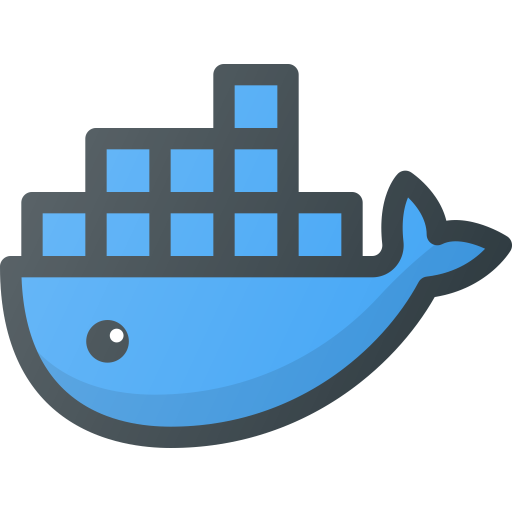
\includegraphics[width=6mm]{docker_icon.jpg}} ([xshift=-10mm,yshift=-9mm]interior.north west);
    }
}

\newtcblisting{bnflisting}[1][]{%
    #1,
    listing options={
        language=bnf,
        basicstyle=\ttfamily\small,
        breaklines=true,
        showstringspaces=false,
    },
    fonttitle=\ttfamily\small,
    underlay unbroken and first={%
        \path[draw=none] (interior.north west) rectangle node[white]{
\includegraphics[width=5mm]{bnf_file.png}} ([xshift=-10mm,yshift=-10mm]interior.north west);
    }
}

\newtcblisting{pythonlisting}[1][]{%
    #1,
    listing options={
        language=Python,
        basicstyle=\ttfamily\small,
        breaklines=true,
        showstringspaces=false,
        keywordstyle=\color{blue}\bfseries,
        escapeinside={(*}{*)}
    },
    fonttitle=\ttfamily\small,
    underlay unbroken and first={%
        \path[draw=none] (interior.north west) rectangle node[white]{
\includegraphics[width=5mm]{python_icon.png}} ([xshift=-10mm,yshift=-10mm]interior.north west);
    }
}

\newtcblisting{rpilisting}[1][]{%
    listing options={
        language=BashPrompt,
        basicstyle=\ttfamily\small,
        tabsize=2,
        inputencoding=utf8,
        #1
    },
    underlay unbroken and first={%
        \path[draw=none] (interior.north west) rectangle node[white]{
\includegraphics[width=8mm]{raspi_icon.png}} ([xshift=-10mm,yshift=-10mm]interior.north west);
    }
}

\tcbset{
    enhanced jigsaw,
    breakable,
    listing only,
    boxsep=-1pt,
    top=-1pt,
    bottom=-0.5pt,
    right=-0.5pt,
    overlay first={
        \node[black!50] (S) at (frame.south) {\Large\ding{34}};
        \draw[dashed,black!50] (frame.south west) -- (S) -- (frame.south east);
    },
    overlay middle={
        \node[black!50] (S) at (frame.south) {\Large\ding{34}};
        \draw[dashed,black!50] (frame.south west) -- (S) -- (frame.south east);
        \node[black!50] (S) at (frame.north) {\Large\ding{34}};
        \draw[dashed,black!50] (frame.north west) -- (S) -- (frame.north east);
    },
    overlay last={
        \node[black!50] (S) at (frame.north) {\Large\ding{34}};
        \draw[dashed,black!50] (frame.north west) -- (S) -- (frame.north east);
    },
%    before={\vspace{5pt}},
%    after={\par\vspace{\parskip}\noindent}  %% do you really need \vspace{\baselineskip}?
}

\newcommand*{\inlineimg}[1]{%
    \raisebox{-.3\baselineskip}{%
        \includegraphics[
            height=\baselineskip,
            width=\baselineskip,
            keepaspectratio,
        ]{#1}%
    }%
}

\def\inline{\lstinline[basicstyle=\ttfamily]}

% Downloads Table
\usepackage{pgfplots}
\usepackage{filecontents}
\usetikzlibrary{pgfplots.dateplot}

\begin{filecontents}{hatchery_downloads.csv}
Category,Downloads
2017-12-01,25
2018-01-01,42
2018-02-01,64
2018-03-01,51
2018-04-01,37
2018-05-01,51
2018-06-01,64
2018-07-01,829
2018-08-01,674
2018-09-01,930
2018-10-01,861
2018-11-01,718
2018-12-01,835
2019-01-01,805
2019-02-01,1019
2019-03-01,1707
2019-04-01,1379
2019-05-01,790
\end{filecontents}

%% Packages utiles.
\usepackage{amssymb,subfigure,icomma}
\usepackage[labelfont=bf, width=\linewidth]{caption}

\def\chapterautorefname{Chapter}
\hypersetup{colorlinks=true,allcolors=black}
\usepackage{hypcap}
\usepackage{bookmark}

\newtheorem{cor}{\corollaryname}[section]
\newtheorem{deff}[cor]{\definitionname}
\newtheorem{ex}[cor]{\examplename}
\newtheorem{lem}[cor]{\lemmaname}
\newtheorem{prop}[cor]{Proposition}
\newtheorem{rem}[cor]{\remarkname}
\newtheorem{theo}[cor]{\theoremname}

\numberwithin{equation}{section}
\numberwithin{table}{chapter}
\numberwithin{figure}{chapter}

\renewcommand{\baselinestretch}{1.5}

\begin{document}

\version{1}

\title{Programming tools for intelligent systems\\
\small{with a case study in autonomous robotics}}

\author{Breandan Considine}

\copyrightyear{2019}

\department{D\'epartement d'informatique et de recherche op\'erationnelle}

\president{Nom du pr\'esident du jury}

\directeur{Nom du directeur de recherche}

%%\codirecteur{Nom du co-directeur}         % s'il y a lieu

\membrejury{Nom du membre de jury}

%%\examinateur{Nom de l'examinateur externe}   %obligatoire pour la these

%% \membresjury{Deuxième membre du jury}  % s'il y a lieu

%%  \plusmembresjury{Troisième membre du jury}    % s'il y a lieu

%%\repdoyen{Nom du représentant du doyen} %obligatoire pour la these

\dateacceptation{La date d'acceptation}

%%
%% Voici les disciplines possibles (voir avec votre directeur):
%% \sujet{statistique},
%% \sujet{mathématiques}, \orientation{mathématiques appliquées},
%% \orientation{mathématiques fondamentales}
%% \orientation{mathématiques de l'ingénieur} et
%% \orientation{mathématiques appliquées}

\sujet{Discipline}
%%\orientation{orientation}%Ce champ est optionnel

%%
%% Fin des variables à définir. La commande \maketitle créera votre
%% page titre.

\pagenumbering{roman}
\maketitle

% Pour générer la deuxième page titre, il faut appeler à nouveau \maketitle
% Cette page est optionnelle et son inclusion est laissé à la discrétion
% de l'étudiant et du directeur de recherche, ou de tout autre instance
% d'autorité.
%%\maketitle

%%------------------------------------------------- %
%%              pages iv                            %
%%------------------------------------------------- %

\chapter*{Summary}

%%------------------------------------------------- %
%%        page v --- Table de matieres              %
%%------------------------------------------------- %

% Pour un mémoire en anglais, changer pour
% \anglais. Noter qu'il faut une permission
% pour écrire son mémoire en anglais.
\anglais
% \cleardoublepage termine la page actuel et force TeX
% a poussé les éléments flottant (fig., tables, etc.) sur
% la page (normalement TeX les garde en suspend jusqu'à ce
% qu'il trouve un endroit approprié). Avec l'option <twoside>,
% la commande s'assure que la prochaine page de texte est sur
% le recto, pour l'impression. On l'utilise ici
% pour que TeX sache que la table des matières etc. soit
% sur la page qui suit.
%% TABLE DES MATIÈRES
\cleardoublepage
\pdfbookmark[chapter]{\contentsname}{toc}  % Crée un bouton sur
% la bar de navigation
\tableofcontents
% LISTE DES TABLES
\cleardoublepage
\phantomsection  % Crée une section invisible (utile pour les hyperliens)
\listoftables
% LISTE DES FIGURES
\cleardoublepage
\phantomsection
\listoffigures

\NoChapterPageNumber
\cleardoublepage
\pagenumbering{arabic}

\welldone{\chapter{Introduction}\label{ch:introduction}}

\setlength{\epigraphwidth}{0.85\textwidth}
\epigraph{There is a race between the increasing complexity of the systems we build and our ability to develop intellectual tools for understanding their complexity. If the race is won by our tools, then systems will eventually become easier to use and more reliable. If not, they will continue to become harder to use and less reliable for all but a relatively small set of common tasks. Given how hard thinking is, if those intellectual tools are to succeed, they will have to substitute calculation for thought.}{\begin{flushright}--Leslie Lamport\end{flushright}}

Computational complexity is of such concern in computer science that a great deal of the field is dedicated to understanding it through the lens of function analysis and information theory. In software engineering, researchers are primarily interested in the complexity of building software -- the digital manifestation of algorithms on physical hardware. One kind of software complexity is the cognitive effort required to understand a program.\footnote{This can be approximated by various metrics like cyclomatic or Halstead complexity.} While today's software is becoming rapidly more intelligent, it shows few signs of becoming more intelligible. Better tools are needed for managing the complexity in building software systems.

\textit{The objective of this thesis is to develop methods that reduce the cognitive effort required to build intelligent systems, using developer tools, programming language abstractions, automated testing, and virtualization technology.}

Broadly speaking, intelligent systems differ from ordinary software systems in that they enable machines to detect patterns, perform tasks, and solve problems which they are not explicitly programmed to solve and which human experts were previously incapable of solving by hard-coding explicit rules. Typically, these systems are able to:\\
%
\begin{enumerate}
    \item learn generalizable rules by processing large amounts of data
    \item tune a large number of free parameters (thousands to billions)
    \item outperform well-trained humans in domain-specific tasks
\end{enumerate}
%
While the idea of intelligent systems has existed for decades, three critical developments made modern intelligent systems ultimately successful. First, computer processing power has become faster, cheaper, and much more readily available. Similarly, the digitalization of new datasets has made vast amounts of information available, and data storage costs have plummeted dramatically. (A \$5 thumb drive today has 200 times more storage capacity than a 2,000 pound, 5 MB, IBM hard drive that leased for \$3,000 per month in 1956.) Most importantly, has been the development of more efficient learning algorithms.

In recent years, computer science and software engineering has made significant strides in building and deploying intelligent systems. Nearly every mobile computer in the world is able to detect objects in images, perform speech-to-text and language translation. These breakthroughs were the direct result of fundamental progress in neural networks and representation learning. Also key to the success of modern intelligent systems was the adoption of collaborative open source practices, pioneered by the software engineering community. Software engineers developed automatic differentiation libraries like Theano~\citep{theano}, Torch~\citep{collobert2002torch} and Caffe~\citep{jia2014caffe}, and built many popular simulators for reinforcement learning, the ease of use and availability of which was crucial for popularizing deep learning techniques.

Intelligent systems are widely deployed in virtual settings like data science and cloud services. But even with the tremendous success of machine learning algorithms in fully-observable domains like image recognition and speech processing, intelligent systems have yet to become widely adopted in robotics at the time of writing this thesis. This dilemma can be partly attributed to various theoretical problems such as domain adaption and transfer learning. Yet with the exponential increase in processing power, proven capabilities of modern learning algorithms, and decades-long research into physically-embodied intelligent agents, we should have more progress to show. Why has this goal evaded researchers for so long? One reason, we conjecture, is a lack of programming tools and abstractions for designing, developing, deploying and evaluating intelligent systems. In practice, these activities consume a large amount of cognitive effort without the right set of tools and abstractions.

In this thesis, we explore several tools that facilitate the process of building intelligent systems, and which reduce the cognitive effort required to understand an intelligent program. First, we demonstrate an integrated development environment that assists users writing robotics software (\autoref{ch:hatchery}). Next, we show a type-safe domain-specific language for differentiable programming, an emerging paradigm in deep learning (\autoref{ch:kotlingrad}). To test this application, we use a set of techniques borrowed from property-based testing~\citep{fink1997property} and adversarial learning~\citep{lowd2005adversarial} (\autoref{ch:difftest}). Docker containers~\citep{merkel2014docker} are used to automate the building, testing and deployment of reproducible robotics applications on heterogeneous hardware platforms (\autoref{ch:ducker}). Finally, as a proof of concept for these ideas, we build an intelligent system comprised of a mobile autonomous vehicle and an Android mobile application, using the tools previously described (\autoref{ch:case-study}).

\section{Stages in the software development lifecycle}\label{sec:sldc-stages}

\begin{figure}
    \centering
    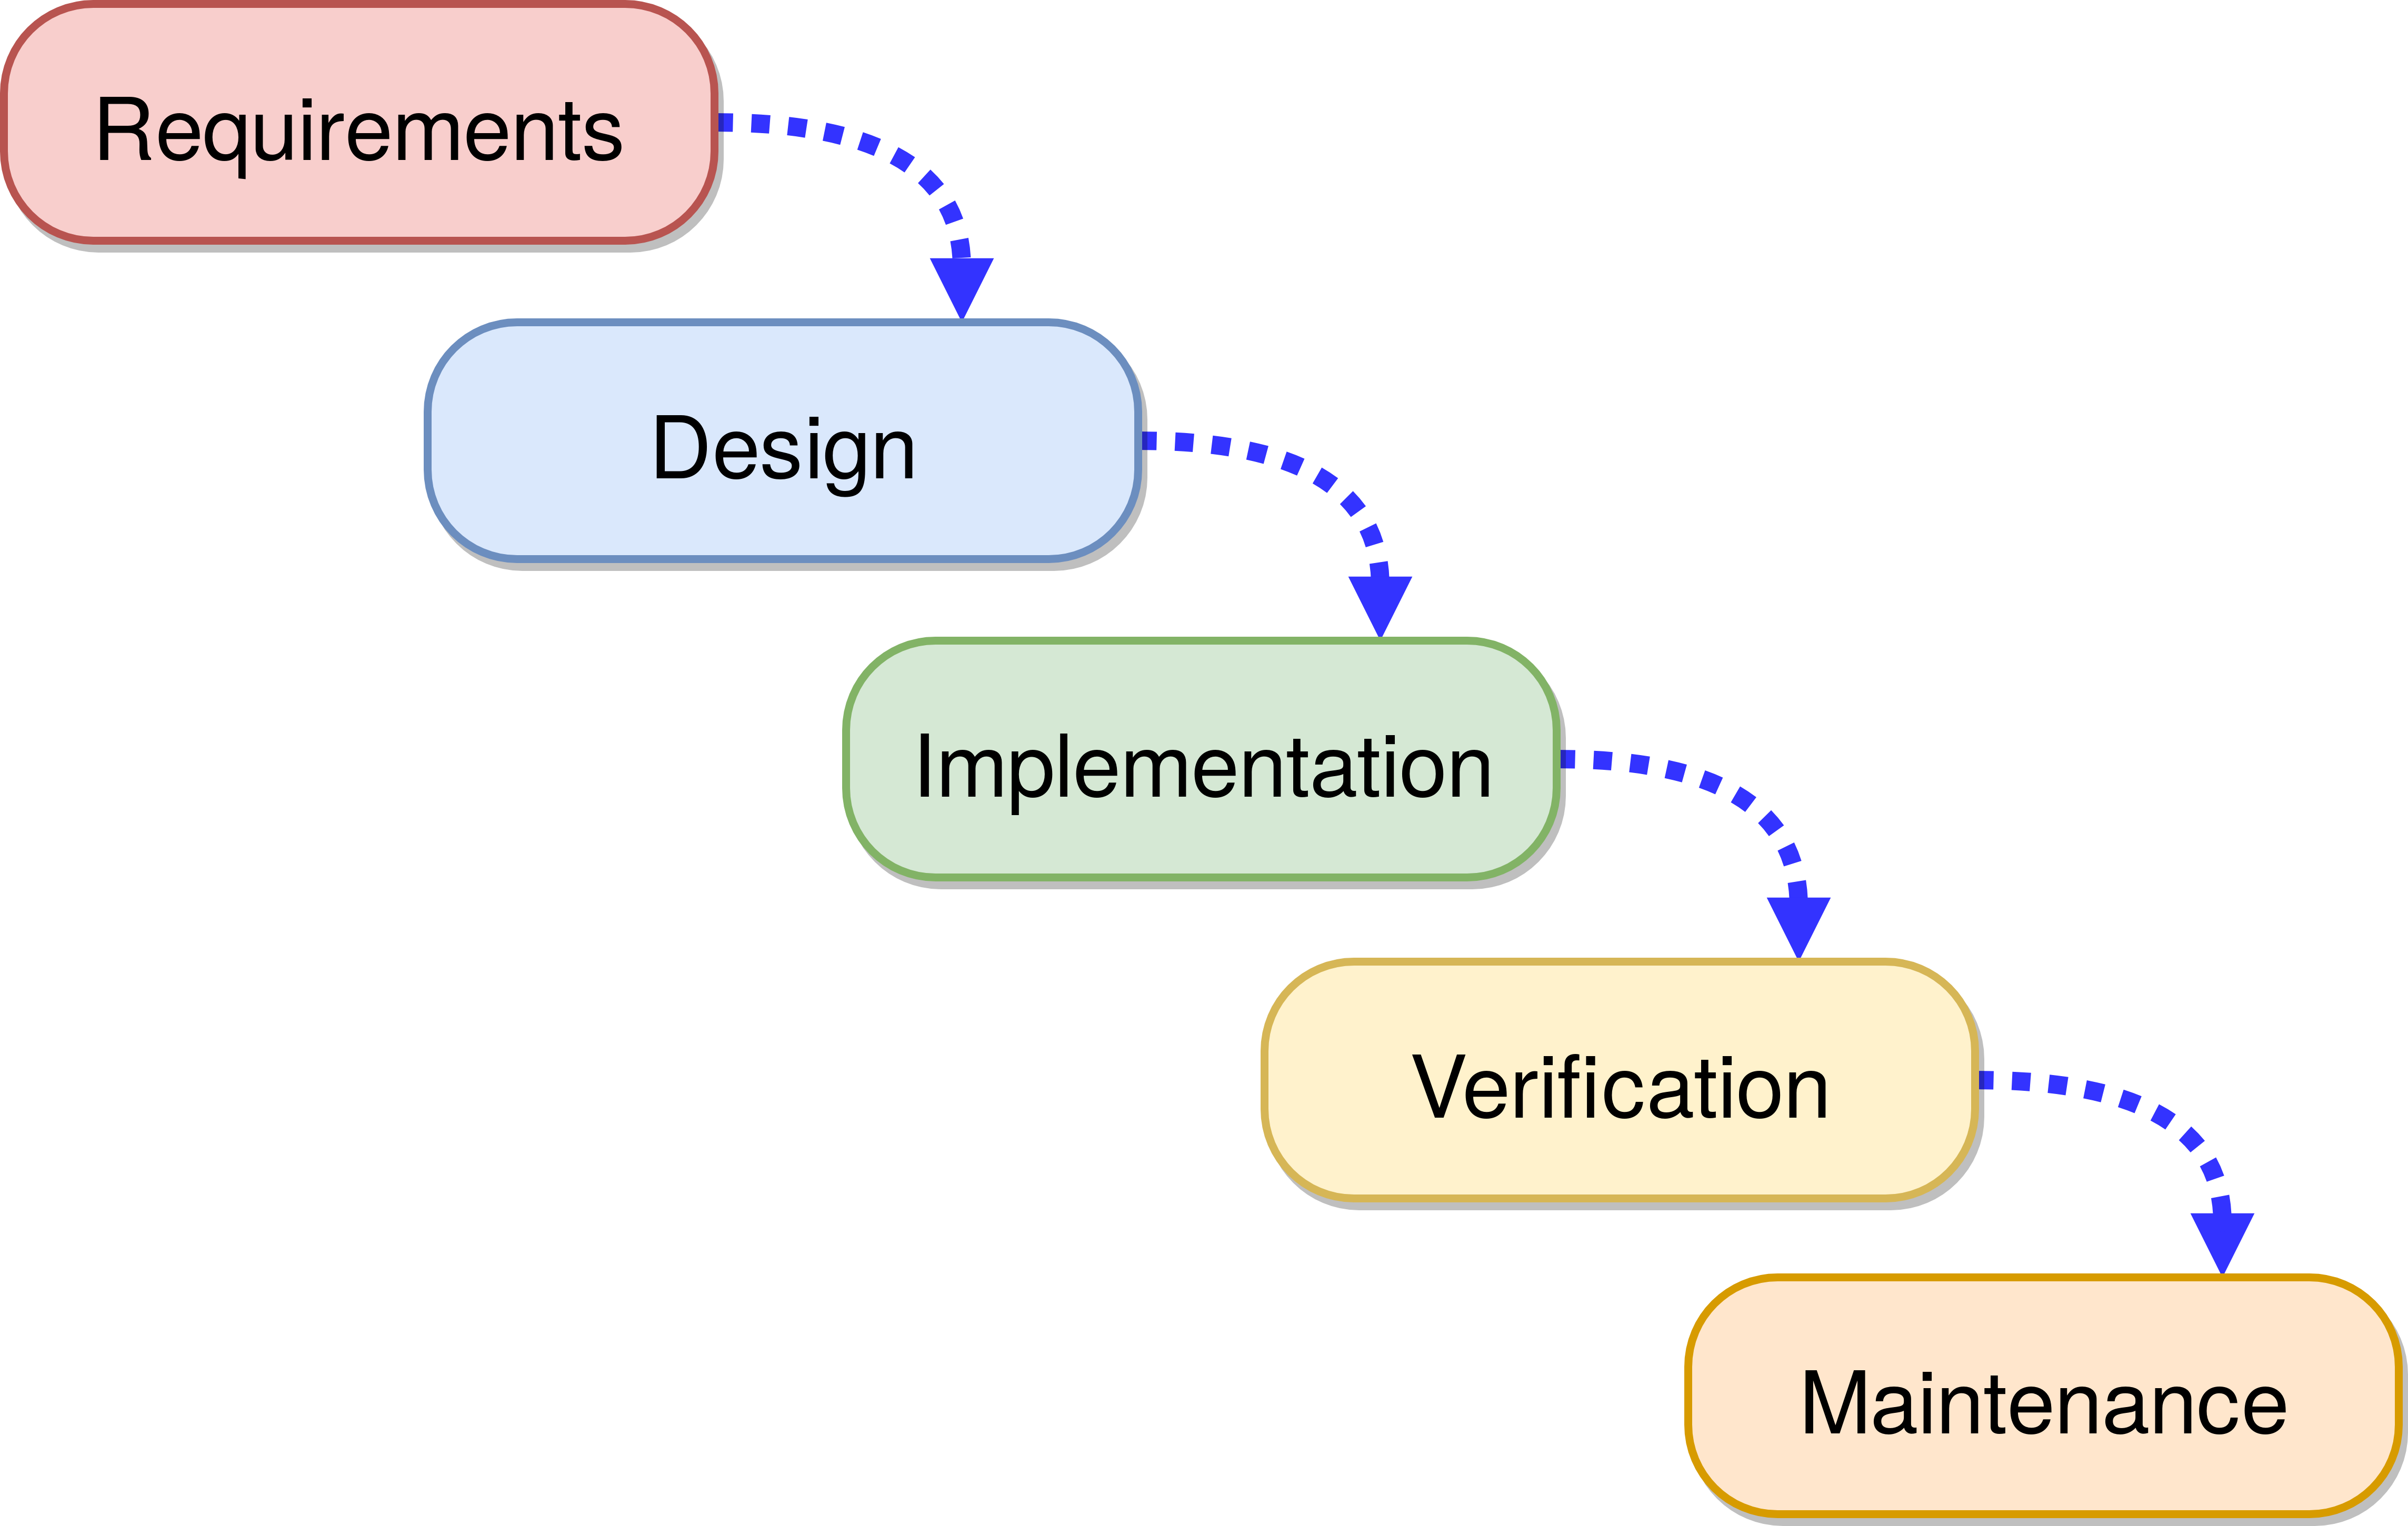
\includegraphics[width=0.70\textwidth]{waterfall_diagram.png}
    \caption{Royce's original Waterfall model, originally intended to describe the software development process, but the same sequence can be found in most engineering disciplines. We use it to help guide our discussion and frame our work inside of this process model.\vspace{-10pt}}
    \label{fig:waterfall_model}
\end{figure}

In traditional software engineering, the Waterfall Model (\autoref{fig:waterfall_model}) is a classical software process model comprised of five stages. While the Waterfall Model was an early model in software engineering, the same activities it describes can be found in most engineering process models. We propose contributions to four such areas: design in \autoref{ch:hatchery}, implementation in \autoref{ch:kotlingrad}, verification in \autoref{ch:difftest} and maintenance in \autoref{ch:ducker}.

\section{Designing intelligent systems}

Today's software systems are deeply complex entities. Gone are the days where a solitary programmer, even a very skilled one, could maintain a large software system alone. To effectively scale modern software systems, programmers must pool their mental capacity to form a knowledge graph. Software projects which rely on a small set of maintainers tend to perish due to the so-called \textit{bus factor}~\citep{cosentino2015assessing} -- large portions of the knowledge graph are locked inside someone's head. Successful software projects learn how to distribute this graph and form connections to the outside world. The knowledge graph which accumulates around a software project contains facts, but it also contains workflows for programming, debugging, and delivery -- common paths through the labyrinth of software development. Components of this graph can be committed to writing, but documentation is time-consuming and grows stale over time. What is needed is a system that offers the benefits of documentation without the burdens of maintenance.

The development of software systems has a second component, the social graph. The social graph of a successful software project contains product designers, managers and software engineers who work in concert to build software that is well-designed, cohesive, and highly performant. Sometimes this means revising the specification to accommodate engineering challenges, or rewriting source code to remove technical debt. Software design is a multi-objective optimization process and requires contributors with a broad set of skills and common set of goals. To produce software that approximates the criteria of its stakeholders, developers are asked to provide rapid prototypes, and continuously integrate user feedback. Yet today's software systems are larger and more unwieldy than ever. So finding ways to collaborate more efficiently is critical to building and maintaining intelligent systems.

First, let us consider the mechanical process of writing software with a keyboard.

Integrated development environments (IDEs) can assist developers building complex software applications by automating certain repetitive programming tasks. For example, IDEs perform static analyses and inspections for catching bugs quickly. They provide completion, refactoring and source code navigation, and they automate the process of building, running and debugging programs. While these tasks may seem trivial, their automation promises increased developer productivity by delivering earlier feedback, detecting clerical errors, and allows developers to focus on fundamental design tasks. Rather than being forced to concentrate on the structure and organization of text, if developers are able to manipulate code at a semantic level, they will be much happier and more productive. Furthermore, by automating mechanical tasks in software development, these tools allow developers to direct their attention to the fundamental activity of writing and understanding programs.

But what are IDEs really doing? They are guiding developers through the knowledge graph of a software project. Consider what a new developer must learn to get up to speed: in addition to learning the language, developers must learn to use libraries and frameworks (arguably languages in their own right). They must become familiar with command line tools for software development, from build tools to version control and continuous integration. They must become familiar with the software ecosystem, programming styles, conventions and development workflows. And they must learn how to collaborate on a distributed team of developers. By automating common tasks in an interactive programming environment and making the graph connectivity explicit through document markup~\citep{goldfarb1981generalized} and projectional editing~\citep{voelter2014towards}, a well-designed IDE is a tool for graph traversal. It should come as no surprise IDEs are really graph databases.

In some aspects, the development of intelligent systems is no different than classical software engineering. The same principles and best-practices which guide software engineering are also applicable to intelligent systems. And the same activities, from design to maintenance will continue to play an important role in building intelligent systems. But in other respects, the generic programming tools used to develop traditional software will require domain-specific adaptations for learning systems to become truly first class citizens in the next generation of intelligent software, particularly in the case of robotics development.

Towards that goal, we developed an IDE for the Robot Operating System (ROS) called \href{https://github.com/duckietown/hatchery}{Hatchery}. It supports a number of common workflows for ROS development, such as creating ROS nodes, Gazebo simulator integration, support for remote debugging, static analysis, autocompletion and refactoring. In \autoref{ch:hatchery} we discuss the implementation of these features and some of the challenges of building language support, programming tools and integrating with the ROS middleware. We argue that such tools reduce the cognitive complexity of building ROS applications by adopting explicit coding conventions, annotating unstructured text and automating repetitive development tasks.

\section{Implementation: Languages and compilers}

In the early days of machine learning, it was widely believed the development of human-level intelligence simply required a sufficiently descriptive first-order logic. By accumulating a database of facts and their relations, researchers believed they could use symbolic reasoning to bypass learning altogether. This rule-based approach dominated a large portion of early research in artificial intelligence and considerable effort was poured into the creation of domain-specific ontologies to capture human knowledge. Despite the best efforts of roboticists, signal processing engineers and natural language researchers, \textit{expert systems} were unable to scale to real-world applications, causing a great disillusionment in A.I. research for a number of decades. While computer scientists underestimated the difficulty of \text{learning}, expert systems excelled in areas where current machine learning systems struggle such as classical reasoning and interpretability, and there is reason to believe these ideas were ahead of their time.

What did finally work, is the idea of connectionist learning. By nesting random function approximators, called perceptrons, and updating the free parameters using backpropagation~\citep{werbos1990backpropagation, rumelhart1988learning}, the resulting system is capable of learning a surprising amount of intelligent behavior. The approach, termed artificial neural networks (ANNs), can be traced back to the mid-20th century~\citep{ivakhnenko1965cybernetic, rosenblatt1958perceptron}, but was not fully-realized in silico until after the widespread availability of cheap computing and large datasets~\citep{lecun2015deep}. In theory, a single layer of nesting is able to approximate any continuous differentiable function~\citep{hornik1989multilayer}, but in practice, learning requires composing many such approximators in a deeply nested fashion, hence the term, \textit{deep neural networks} (DNNs). The importance of depth was suspected for many years, but the original backpropagation algorithm had difficulty training DNNs due to the vanishing gradient problem~\citep{bengio1994learning}. Solving this problem required a number of adaptations and many years to fully debug. It was not until 2013 when deep learning was competitive with humans in a number of domains.

While it took fundamental research in deep learning to realize the connectionist blueprint, the success of modern deep learning can be partly attributed to software tools for calculating mathematical derivatives, a key step in the backpropagation algorithm. Although it has yet not been established if or how derivatives might be calculated in biological circuits, derivatives are essential for ANN training. For many years, the symbolic form of these derivatives were analytically derived when prototyping a new neural network architecture, a tedious and error-prone process. There is a well-known algorithm in the scientific computing community dating back to the 1970s, called \textit{automatic differentiation} (AD)~\citep{linnainmaa1970representation, griewank1989automatic}, which is able to calculate derivatives for arbitrary differentiable functions. But surprisingly, it was not until much later, after the development of Theano~\citep{theano} when AD became widely adopted in the machine learning community. This library alone greatly accelerated the pace of deep learning research and spurred the development of others like TensorFlow~\citep{abadi2016tensorflow} and PyTorch~\citep{paszke2017automatic}.

Intelligent systems engineers must think carefully about languages and abstractions. If developers are required to implement backpropogation by hand, they will have scarce time to think about the high-level characteristics of these systems. Similarly, if programming abstractions are too specific, small variations will require costly reimplementation. This is no different from traditional software engineering -- as engineers, we need to choose the right abstractions for the task at hand. Too low-level and the design is lost in the details, too abstract and the details are lost completely. With deep learning, the necessity of choosing good abstractions is even more important, as the relationship of between source code and runtime behavior is already difficult to debug, due to the complexity of neural networks and array programming. One component of that complexity can be found in the type system.

The majority of existing AD frameworks for machine learning are implemented in dynamically typed languages like Python, Lua and JavaScript, with some early implementations including projects like Theano, Torch and Caffe. Similar ideas have arisen in statically-typed, functional languages, such as Haskell (Stalin$\nabla$~\citet{pearlmutter2008using}), Scala (Nexus~\citet{chen2017typesafe}), F\# (DiffSharp~\citet{baydin-diffsharp}), Swift~\citep{swift}, et al., but most of these are unable to check the shape of multidimensional arrays in their type system, and those which do are typically implemented in experimental languages with sophisticated type-level programming features. In our work, we demonstrate the viability of shape-checked differentiable programming in a widely-used language with parametric types. This ensures that programs on matrices, if they compile, are the correct shape can be numerically evaluated at runtime.

Kotlin$\nabla$ is an embedded domain-specific language (eDSL) for differentiable programming in a language called Kotlin, a statically-typed programming language with support for asynchronous programming and multi-platform compilation. In Kotlin$\nabla$ (\autoref{ch:kotlingrad}), we describe an algebraically-grounded implementation of forward-mode automatic differentiation with shape-safe tensor operations. Our approach differs from existing AD frameworks in that Kotlin$\mathbf{\nabla}$ is the first shape-safe AD library fully compatible with the Java type system, requiring no metaprogramming, reflection or compiler intervention to use.

\section{Testing and validation}

Most naturally arising phenomena, particularly those related to vision, planning and locomotion are high dimensional creatures. Richard Bellman famously coined this problem as the ``curse of dimensionality''. Our physical universe is populated by problems which are simple to pose, but impossible to solve inside of it. Claude Shannon, a contemporary of Bellman, calculated the number of unique chess games to exceed $10^{120}$, more than the number of atoms in the universe by approximately 40 orders of magnitude~\citep{shannon1950xxii}. At the time, it was believed that such problems would be insurmountable without a fundamental change in algorithms or computing machinery. Indeed, while Bellman or Shannon did not live to see the day, it took only half a century of progress in computer science before solutions to problems with the same order of complexity, first solved in the Cambrian explosion 541 million years ago, were approximated to a competitive margin in modern computers.

While computer science has made enormous strides in solving the common cases, Bellman's curse of dimensionality still haunts the long tail of machine learning, particularly for distributions that are highly dispersed. Because the dimensionality of many real world functions that we would like to approximate is intractably large, it is difficult to verify the behavior of a candidate solution in all regimes, especially in settings where failure is rare but catastrophic. According to some studies, humans drivers average 1.09 fatalities per hundred million miles~\citep{kalra2016driving}. A new software build for an autonomous vehicle would need to accumulate 8.8 billion miles of driving in order to approximate the fatality rate of a human operator to within 20\% with a 95\% confidence interval. Deploying such a scheme in the real world would be logistically, not to mention ethically, problematic.

Realistically speaking, intelligent systems need better ways to practice their skills and probe the effectiveness of a candidate solution within a limited computational budget, without harming humans in the process. The goal of this testing is to highlight errors, but ultimately to provide feedback to the system. In software engineering, the real system under test are the ecosystem of humans and machines which provide each other's means of subsistence. The success of this arrangement depends on an external testing mechanism to enforce a minimum bar of rigor, typically some form of hardware- or human-in-the-loop testing. If the testing mechanism is not somehow opposed to the system under test, an intelligent system can deceive itself, which is neither in the system's nor its users' best interests.

In this \autoref{ch:difftest} we present preliminary work in adversarial fuzz testing, building on prior literature in adversarial learning, metamorphic and property-based testing. A similar technique is used for testing the numerical correctness of Kotlin$\nabla$'s implementation. We present a simple algorithm for property-based shrinking using projected gradient descent and suggest several future directions for improvement.

\section{Software reproducibility and maintenance}

One of the challenges of building intelligent systems and programming in general, is the problem of reproducibility. Software reproducibility has several challenging aspects, including hardware compatibility, operating systems, file systems, build systems, and runtime determinism. While writing programs and feeding them directly into a computer may have once been common practice, today's source code is far too removed from its mechanical realization to be meaningfully executed in isolation. Today's handwritten programs are like schematics for a traffic light -- built inside a factory, and which require a city's-worth of infrastructure, cars, and traffic laws to serve their intended purpose. Like traffic lights, source code does not exist in a vacuum -- built by compilers, interpreted by virtual machines, executed inside an operating system, and which following a specific communication protocol -- programs are essentially meaningless abstractions outside this context.

As necessary in any good schematic, much of the information required to build a program is divided into layers of abstraction. Most low-level instructions carried out by a computer during the execution of a program were not written nor intended to be read by the programmer and have long since been automated and forgotten. In a modern programming language like Java, C\# or Python, the total information required to run a simple program often numbers in the trillions of bits. A portion of that data pertains to the software for building and running programs, including the build system, software dependencies, and development tools. Part of the data pertains to the operating system, firmware, drivers, and embedded software. For most programs, such as those found in a typical GitHub repository\footnote{c.f. \url{https://help.github.com/en/articles/what-is-my-disk-quota}}, a vanishingly small fraction correspond to the source code itself.

Applied machine learning shares many of the same practical challenges as traditional software development, with source code, release and dependency management. The current process of training a deep learning model can be seen as particularly long compilation step, but it differs significantly in that the source code is a high-level language which does not directly describe the computation being performed, but is a kind of meta-meta-program. The first meta-program describes the connectivity of a large directed graph (i.e.~ a computation graph or probabilistic graphical model), parameterized by weights and biases. The tuning of those parameters is another meta-program, describing the sequence of operations required to approximate a program which we do not have access, save for some input-output examples. Emerging techniques in meta-learning and hyper-parameter optimization (e.g.~differentiable architecture search~\citep{liu2018darts}) add even further meta-programming layers to this stack, by searching over the space of directed graphs themselves.

Hardware manufacturers have developed a variety of custom silicon to train and run these programs rapidly. But unlike most programming, deep learning is a much simpler model of computation -- so long as a computer can add and multiply, it has the ability to run a deep neural network. Yet due to the variety of hardware platforms which exist and the software churn associated with them, reproducing deep learning models can be painstakingly difficult on new hardware, even with the same source code and dependencies. Many graph formats, or \textit{intermediate representations} (IRs) in compiler parlance, promise hardware portability but if developers are not careful, their models may not converge during training, or may produce different results on different hardware. Complicating the problem, IRs are produced by competing vendors, with competing chips and incompatible standards (e.g.~MLIR~\citep{mlir}, ONNX~\citep{bai2019}, nGraph~\citep{cyphers2018intel}, Glow~\citep{rotem2018glow}, TVM~\citep{tvm2018} et al.) While some have tried to leverage existing compilers such as GHC~\citep{elliott2018simple} or DLVM/LLVM~\citep{wei2017dlvm}, there are few signs of interoperability at the time of writing this thesis.

At the end of the day, researchers need to reproduce the work of other researchers, but the mental effort of re-implementing their abstractions can be tedious and detrimental towards scientific progress. Since it is necessary to reuse programs written by others, it would be convenient to have tools for reproducibility and incremental development. Fortunately, this is the same problem software developers have been attempting to solve for many years, through open source software. But source control management (SCM) alone is insufficient, since SCM tools are primarily intended for text. While text-based representations may be temporarily stable, as dependencies are periodically updated and rebuilt, important details about the original development environment can be misplaced. To reproduce a program in its entirety, we need a snapshot of all digital information available to the computer at the time of its execution, and ideally, the physical computer itself. Short of that, the minimal set of dependencies and a close replica is essential.

In order to mitigate the effects of software variability and assist the development of intelligent systems on heterogeneous platforms, we use a developer tool called Docker, part of a loosely-affiliated set of tools for build automation and developer operations which we shall refer to as \textit{container infrastructure}. Docker allows developers to freeze a software system and its host environment, allowing developers (e.g.~using a different environment) to quickly reproduce programs on another computer. Docker itself is a technical solution, but also encompasses a set of best-practices which are more procedural in nature. While Docker itself does not address the incompatibility of vendor standards and hardware drivers, it makes these variables explicit, and reduces the difficulty of reproducing software artifacts.

There is a second component to software reproducibility of intelligent systems, at the boundary of software and hardware: simulators. Today's simulators have become increasingly realistic, but most roboticists agree that simulation alone will never be enough to capture the full distribution of real world data. In this view, while simulation can be a useful tool for detecting errors, it cannot fully reproduce all the intricacies of the real world, and must never be used as a surrogate for training on real-world data. Others have suggested a middle road~\citep{bousmalis2018using}, where judicious use of simulator training, alongside domain adaption is a sufficiently rigorous environment for training intelligent systems. Regardless of which view prevails, our goal is to provide rapid feedback to developers, and to make the entire process from testing to deployment as reproducible as possible.

\subsection{Case Study}\label{subsec:case-study}

All great software has a secret recipe: software gets better when its authors use the product. In the best case, the authors are the core users, ideally by choice, if not by necessity. When software engineers are using their own software on a regular basis -- bumping into sharp corners and encountering edge cases firsthand -- the product gets better. When there is an obviously missing feature, it gets implemented. When there is a bug, it gets fixed. It may not be easy to find users are so inclined, or to build software which is so useful, but there must be some overlap in order for good software to become great. Termed ``dogfooding''~\citep{harrison2006eating}, this practice is an effective mechanism for building self-improving cybernetic systems and an important principle for open source software and safety-critical systems. Putting this principle into practice, we, as authors and primary users of these tools, validate their effectiveness by developing a robotics application within an IDE (\autoref{ch:hatchery}), containing Kotlin$\nabla$ code (\autoref{ch:kotlingrad}), tested using adversarial fuzz testing (\autoref{ch:difftest}), and which is built and maintained using the Docker stack (\autoref{ch:ducker}).

\subsection{Iconography}

Throughout this thesis, the following iconography is used to denote: \\
%
\begin{enumerate}
\item[] \inlineimg{laptop_icon.png} &  Shell commands intended for a laptop, or output derived thereof. \\
\item[] \inlineimg{bnf_file.png} & GrammarKit's \inline{.bnf} parsing expression grammar (PEG)~\footnote{GrammarKit usage notes: \url{https://github.com/JetBrains/Grammar-Kit/blob/master/HOWTO.md}} \\
\item[] \inlineimg{docker_icon.jpg} &  Either \inline{Dockerfile}~\footnote{Dockerfile reference: \url{https://docs.docker.com/engine/reference/builder/}} or Docker Compose~\footnote{Compose file reference: \url{https://docs.docker.com/compose/compose-file/}} syntax. \\
\item[] \inlineimg{raspi_icon.png}  &  Shell commands which should be run on a Raspberry Pi. \\
\item[] \inlineimg{duckietown.png}  &  Duckietown Shell (\inline{dts}) commands. \\
\item[] \inlineimg{launch_icon.png}  &  roslaunch \inline{.launch} files. \\
\item[] \inlineimg{python_icon.png}  &  Python source code. \\
\item[] \inlineimg{kotlin_file.png}  &  Kotlin source code.
\end{enumerate}

\medium{\chapter{Design: Programming tools for robotics}\label{ch:hatchery}}
\setlength{\epigraphwidth}{0.78\textwidth}
\epigraph{``The hope is that, in not too many years, human brains and computing machines will be coupled together very tightly, and that the resulting partnership will think as no human brain has ever thought and process data in a way not approached by the information-handling machines we know today.''}{\begin{flushright}--J.C.R. \citet{licklider1960man}, \textit{Man-Computer Symbiosis}\end{flushright}}

In this chapter we will discuss the design and implementation of an integrated development environment (IDE) for building intelligent robotic software. Modern robots are increasingly driven by systems which learn and improve over time. Most researchers would agree that modern robotic systems have not yet achieved biologically competitive sensorimotor capabilities and most intelligent systems are not physically embodied. However, it is our view that any closed-loop control system that is not explicitly programmed to perform a specific task, but which learns it from experience is an \textit{intelligent system}. Furthermore, any closed-loop system with physical motors is a \textit{robotic system}. While research has demonstrated successful applications in both areas separately, it is widely believed the integration of intelligent systems in robotics will be tremendously fruitful when fully realized.

Hatchery is a tool designed to assist programmers writing robotics applications using the ROS middleware. At the time of its release, \href{https://github.com/duckietown/hatchery}{Hatchery} was the first ROS plugin for the IntelliJ Platform \footnote{An IDE platform for C/C++, Python and Android development}, and today, is the most widely used with over 10,000 unique downloads. While the idea is simple, its prior absence and subsequent adoption suggests there is unmet demand for such tools in the development of intelligent software systems, particularly in domain-specific applications like robotics.
%

\begin{figure}
\centering
\begin{tikzpicture}
\begin{axis}[
    ybar, ymin=0,
    ylabel=Downloads,
    date coordinates in=x,
    xmin=2017-12-01,
    xmax=2019-06-01,
    xtick=data,
    xticklabel style={
        rotate=70,
        anchor=near xticklabel,
    },
    xticklabel=\year-\month,
    nodes near coords,
    nodes near coords align={vertical},
    height=0.25\textwidth,
    width=0.95\textwidth,
    enlarge x limits=0.03,
    axis x line*=bottom,
    axis y line*=left,
    tick pos=left,
    compat=newest,
]
\addplot table[col sep=comma, x=Category,y=Downloads]{hatchery_downloads.csv};
\end{axis}
\node[above,font=\large\bfseries] at (current bounding box.north) {Unique Downloads of Hatchery};
\end{tikzpicture}
\caption{Unique downloads of Hatchery between the time of its release and now. Aggregate statistics available here: \url{https://plugins.jetbrains.com/plugin/10290-hatchery}.}
\label{fig:hatchery_downloads}
\end{figure}
%
\section{Introduction to the Robot Operating System}

The Robot Operating System (ROS) is a popular middleware for robotics applications. At its core, ROS provides software infrastructure for distributed messaging, but also includes a set of community-developed libraries and graphical tools for building robotics applications. ROS is not an operating system (OS) in the traditional sense, but it does offer OS-like functionality such as shared memory and inter-process communication. Unlike pure message-oriented systems like DDS and ZMQ, in addition to the communication infrastructure, ROS provides specific APIs for building decentralized robotic systems, particularly those which are capable of mobility. This includes standard libraries for serializing and deserializing geometric data, coordinate frames, maps, sensor messages, and imagery.

The ROS middleware provides several language front-ends for polyglot programming. According to one community census taken in 2018, 55\% of all ROS applications on GitHub are written in C/C++, followed by Python with a 25\%~\citep{Areserio54:online} share. Source code for a typical ROS application contains a mixture of C/C++ and Python code, corresponding to the language preferences in the robotics and machine learning communities. Hatchery is capable of working with most common ROS client libraries, including rosjava for Java, rospy for Python, roscpp for C/C++, and several other language front ends.

\begin{figure}
\centering
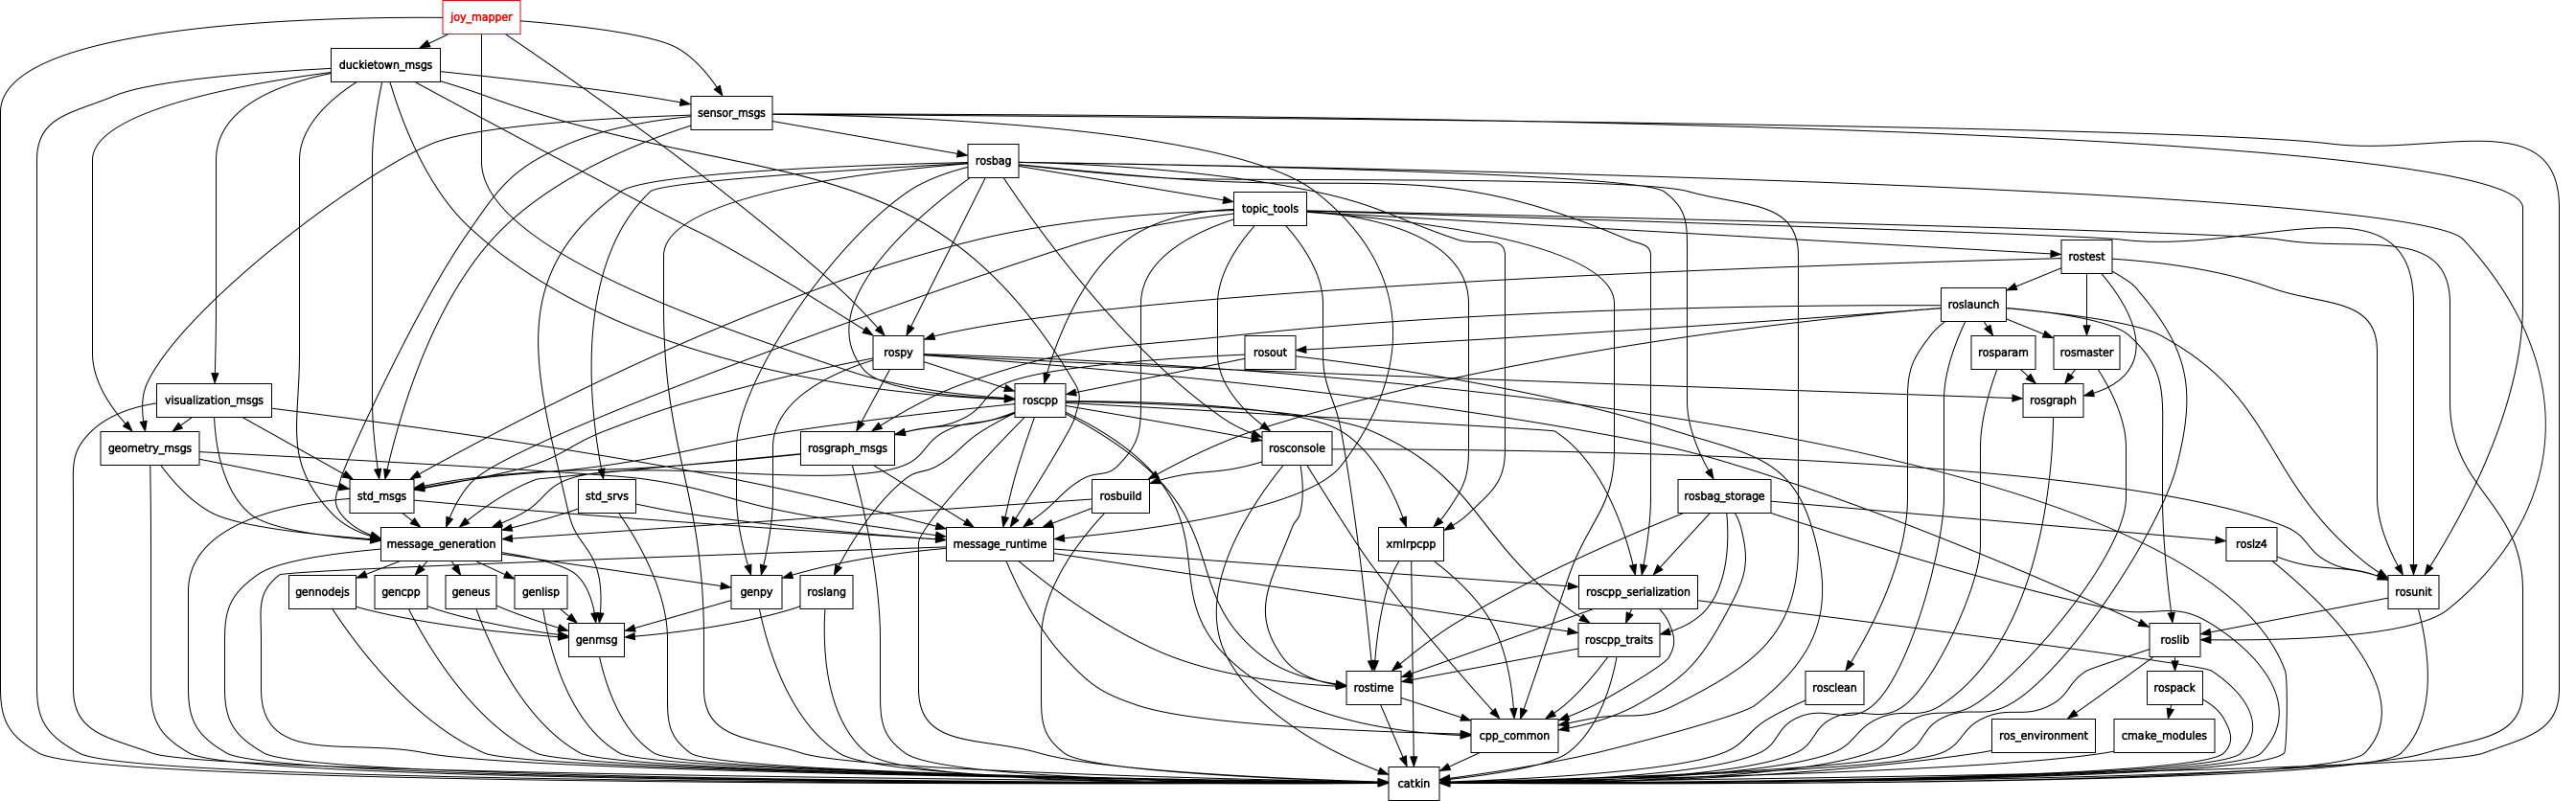
\includegraphics[width=\textwidth]{rqt_dep_graph.png}
\caption{A typical ROS application contains a large graph of dependencies.}
\end{figure}

A typical ROS project has several components, including the source code, configuration files, build infrastructure, compiled artifacts and the deployment environment. To build a simple ROS application, a number of steps are necessary. First, one must install the ROS system, which is only officially supported on Debian-based Linux distributions.\footnote{Detailed installation instructions may be found here: \url{http://wiki.ros.org/ROS/Installation}}
%
Assuming ROS has been installed to the default location, it can be sourced like so:
%
\begin{pclisting}
~$ source /opt/ros/<ROS DISTRO>/setup.[ba]sh
\end{pclisting}
%
A minimal ROS application contains at least one \textit{publisher} and \textit{subscriber}, which pass messages over a shared communication channel. The publisher might be defined as follows:
%
\begin{pythonlisting}[title=./catkin\_ws/src/pubsub/publisher.py]
import rospy
from std_msgs.msg import String

i = 0
pub = rospy.Publisher("channel", String, queue_size=10)
rospy.init_node("publisher", anonymous=True)
rate = rospy.Rate(10)
while not rospy.is_shutdown():
    pub.publish("sent: %s" % i)
    rate.sleep()
    i += 1
\end{pythonlisting}
%
As the publisher writes messages to \inline{channel}, a subscriber can read them off like so:
%
\begin{pythonlisting}[title=./catkin\_ws/src/pubsub/subscriber.py]
def callback(data):
    rospy.loginfo(rospy.get_caller_id() + "received data %s", data.data)

rospy.init_node("subscriber", anonymous=True)
rospy.Subscriber("channel", String, callback)
rospy.spin()
\end{pythonlisting}
%
All ROS packages have launch file, which contain a manifest of available nodes:
%
\begin{launchlisting}[title=./catkin\_ws/src/pubsub/pubsub.launch]
<launch>
<node name="publisher" pkg="pubsub" type="publisher.py" output="screen"/>
<node name="subscriber" pkg="pubsub" type="subscriber.py" output="screen"/>
</launch>
\end{launchlisting}
%
To build and run the application, the following series of commands are required:
%
\begin{pclisting}
~$ cd catkin_ws && catkin_make
\end{pclisting}
%
\begin{pclisting}
~$ rosrun package_name publisher.py
\end{pclisting}
%
\begin{pclisting}
~$ rosrun package_name subscriber.py
\end{pclisting}
%
Rather than interacting with the command line, it would be convenient if there were a graphical tool which could perform all these tasks. Additionally, it would be helpful to detect if there were a navigable reference or typographical error in the launch file:
%
\begin{launchlisting}[title=./catkin\_ws/src/pubsub/pubsub.launch]
<launch>
<node name="publisher" pkg="pubsub" type="(*\color{red}\textbf{\texttt{pubsher.py}}*)" output="screen"/>
<node name="subscriber" pkg="pubsub" type="(*\color{blue}\underline{subscriber.py}*)" output="screen"/>
</launch>
\end{launchlisting}
%
Notice how the typographical error is printed in red and the file reference is underlined in blue, indicating it can be selected. These are the kinds of UI features that IDEs provide.

\section{Prerequisities}

To simply run the tool, users should have the following software dependencies:
%
\begin{enumerate}
    \item MacOS or Debian Linux
    \item Robot Operating System (Electric Emys or later)
    \item Java SE (JRE 8+)
\end{enumerate}
%
ROS users can use the following command to open a ROS project:
%
\begin{pclisting}
~$ git clone https://github.com/duckietown/hatchery && cd hatchery && \
   ./gradlew runIde [-Project="<ABSOLUTE_PATH_TO_ROS_PROJECT>"]
\end{pclisting}
%
Duckietown users can simply use \inline{dts}, the Duckietown Shell:
%
\begin{dtslisting}
dt> hatchery
\end{dtslisting}
%
To build the IDE, some additional tools are helpful. First, is an IDE, which we shall refer to as IDE\textsubscript{0}, and its source code. Assume that IDE\textsubscript{0} exists. In order to build a new IDE, IDE\textsubscript{1}, first load the source code from IDE\textsubscript{0} into IDE\textsubscript{0}. Then, use IDE\textsubscript{0}, to modify, compile and run the source code, which becomes IDE\textsubscript{1}. Iterate as necessary until feature complete.

While valid, this approach has some disadvantages. First, most IDEs are already quite large and cumbersome to download, install, compile, and run. As most auxiliary features are small by comparison, modern IDEs have adopted a modular design, which allows them to load specific packages (i.e.\ \textit{plugins}), as needed. So most developers can skip the first step, and load their plugin, using IDE\textsubscript{0} directly. It is still convenient to have the platform source code for reference purposes, but in most cases this source code is read-only.

For the purposes of this plugin, we use the IntelliJ Platform, a popular platform for cross-language development. By targeting an IDE platform with support for polyglot programming, we are able to focus on programming language-agnostic features in the ROS ecosystem, such as parsing and editing ROS-specific configuration files, build and run configuration and other common development tasks.

\subsection{Refactoring}\label{subsec:refactoring}

Refactoring is a key features in any good IDE, and the essence of refactoring is renaming. Consider what must occur when a user wishes to rename a token in her program, for example the \inline{data} parameter on line \#1 below:
%
\begin{pythonlisting}
def callback(data):
    rospy.loginfo(rospy.get_caller_id() + "received data: %s", data.data)
\end{pythonlisting}
%
If she were using the \inline{vim} text editor, one solution would be to replace all textual occurrences of the string \inline{data} in the file via \inline{:%s/data/msg/g}, with the following result:
%
\begin{pythonlisting}
def callback((*\hl{msg}*)):
    rospy.loginfo(rospy.get_caller_id() + "received (*\hl{msg}*): %s", (*\hl{msg}*).(*\hl{msg}*))
\end{pythonlisting}
%
There were four occurrences of the string \inline{data}, only two of which were valid renaming tokens. Instead, we would like to rename only those identifiers sharing a lexical scope.
%
\newcommand{\cfbox}[2]{
    \colorlet{currentcolor}{.}{
        \color{#1}\fbox{\color{currentcolor}#2}
    }
}

\begin{pythonlisting}
def callback((*\cfbox{red}{data}*)):
    rospy.loginfo(rospy.get_caller_id() + "received data: %s", (*\cfbox{red}{data}*).data)
\end{pythonlisting}

More generally, we would like to rename identifiers used across files and languages in the same project, and doing so requires a richer model of the text in an editor. We need a parser.

\subsection{The Parser}\label{subsec:the-parser}

One of the most important and unappreciated components of an IDE is the parser. Unlike compilers, most IDEs do not use recursive descent or shift-reduce parsers, as they are not well-suited for real-time editing of source code. Edits are typically short, localized changes inside a large file, and are frequently invalid. As the IDE is expected to recover from local errors and provide responsive feedback to users while editing, re-parsing the entire document between edits would be expensive and unnecessary. In order to validate source code undergoing simultaneous modification, special consideration must be taken to ensure robust and responsive parsing.

Incremental methods such as \citet{wagner1997practical,wagner1997incremental} incorporate caching and differential parsing to accelerate the analysis of programs under modification. Fuzzy parsing techniques such as those described in ~\citet{koppler1997systematic} aim to increase the flexibility an robustness of parsing in the presence of local errors. Both of these techniques have played an important role in the development of language-aware programming tools for IDEs and text editors, which must be able to provide rapid and specific feedback whilst the user is typing.

Hatchery can parse URDF, package and launch XML, and \inline{.msg}/\inline{.srv} files.

Here is an excerpt of a ROS interface file grammar:

\begin{bnflisting}
rosInterfaceFile ::= (property|COMMENT)*
property ::= (TYPE KEY SEPARATOR VALUE)|(TYPE KEY) {
pin=3
recoverWhile="recover_property"
mixin="edu.umontreal.hatchery.psi.impl.RosInterfaceNamedElementImpl"
implements="edu.umontreal.hatchery.psi.RosInterfaceNamedElement"
methods=[getType getKey getValue getName setName getNameIdentifier]
}

private recover_property ::= !(TYPE|KEY|SEPARATOR|COMMENT)
\end{bnflisting}

\subsection{Running and debugging}

Assistance for running ROS applications.

\begin{figure}
    \centering
    \frame{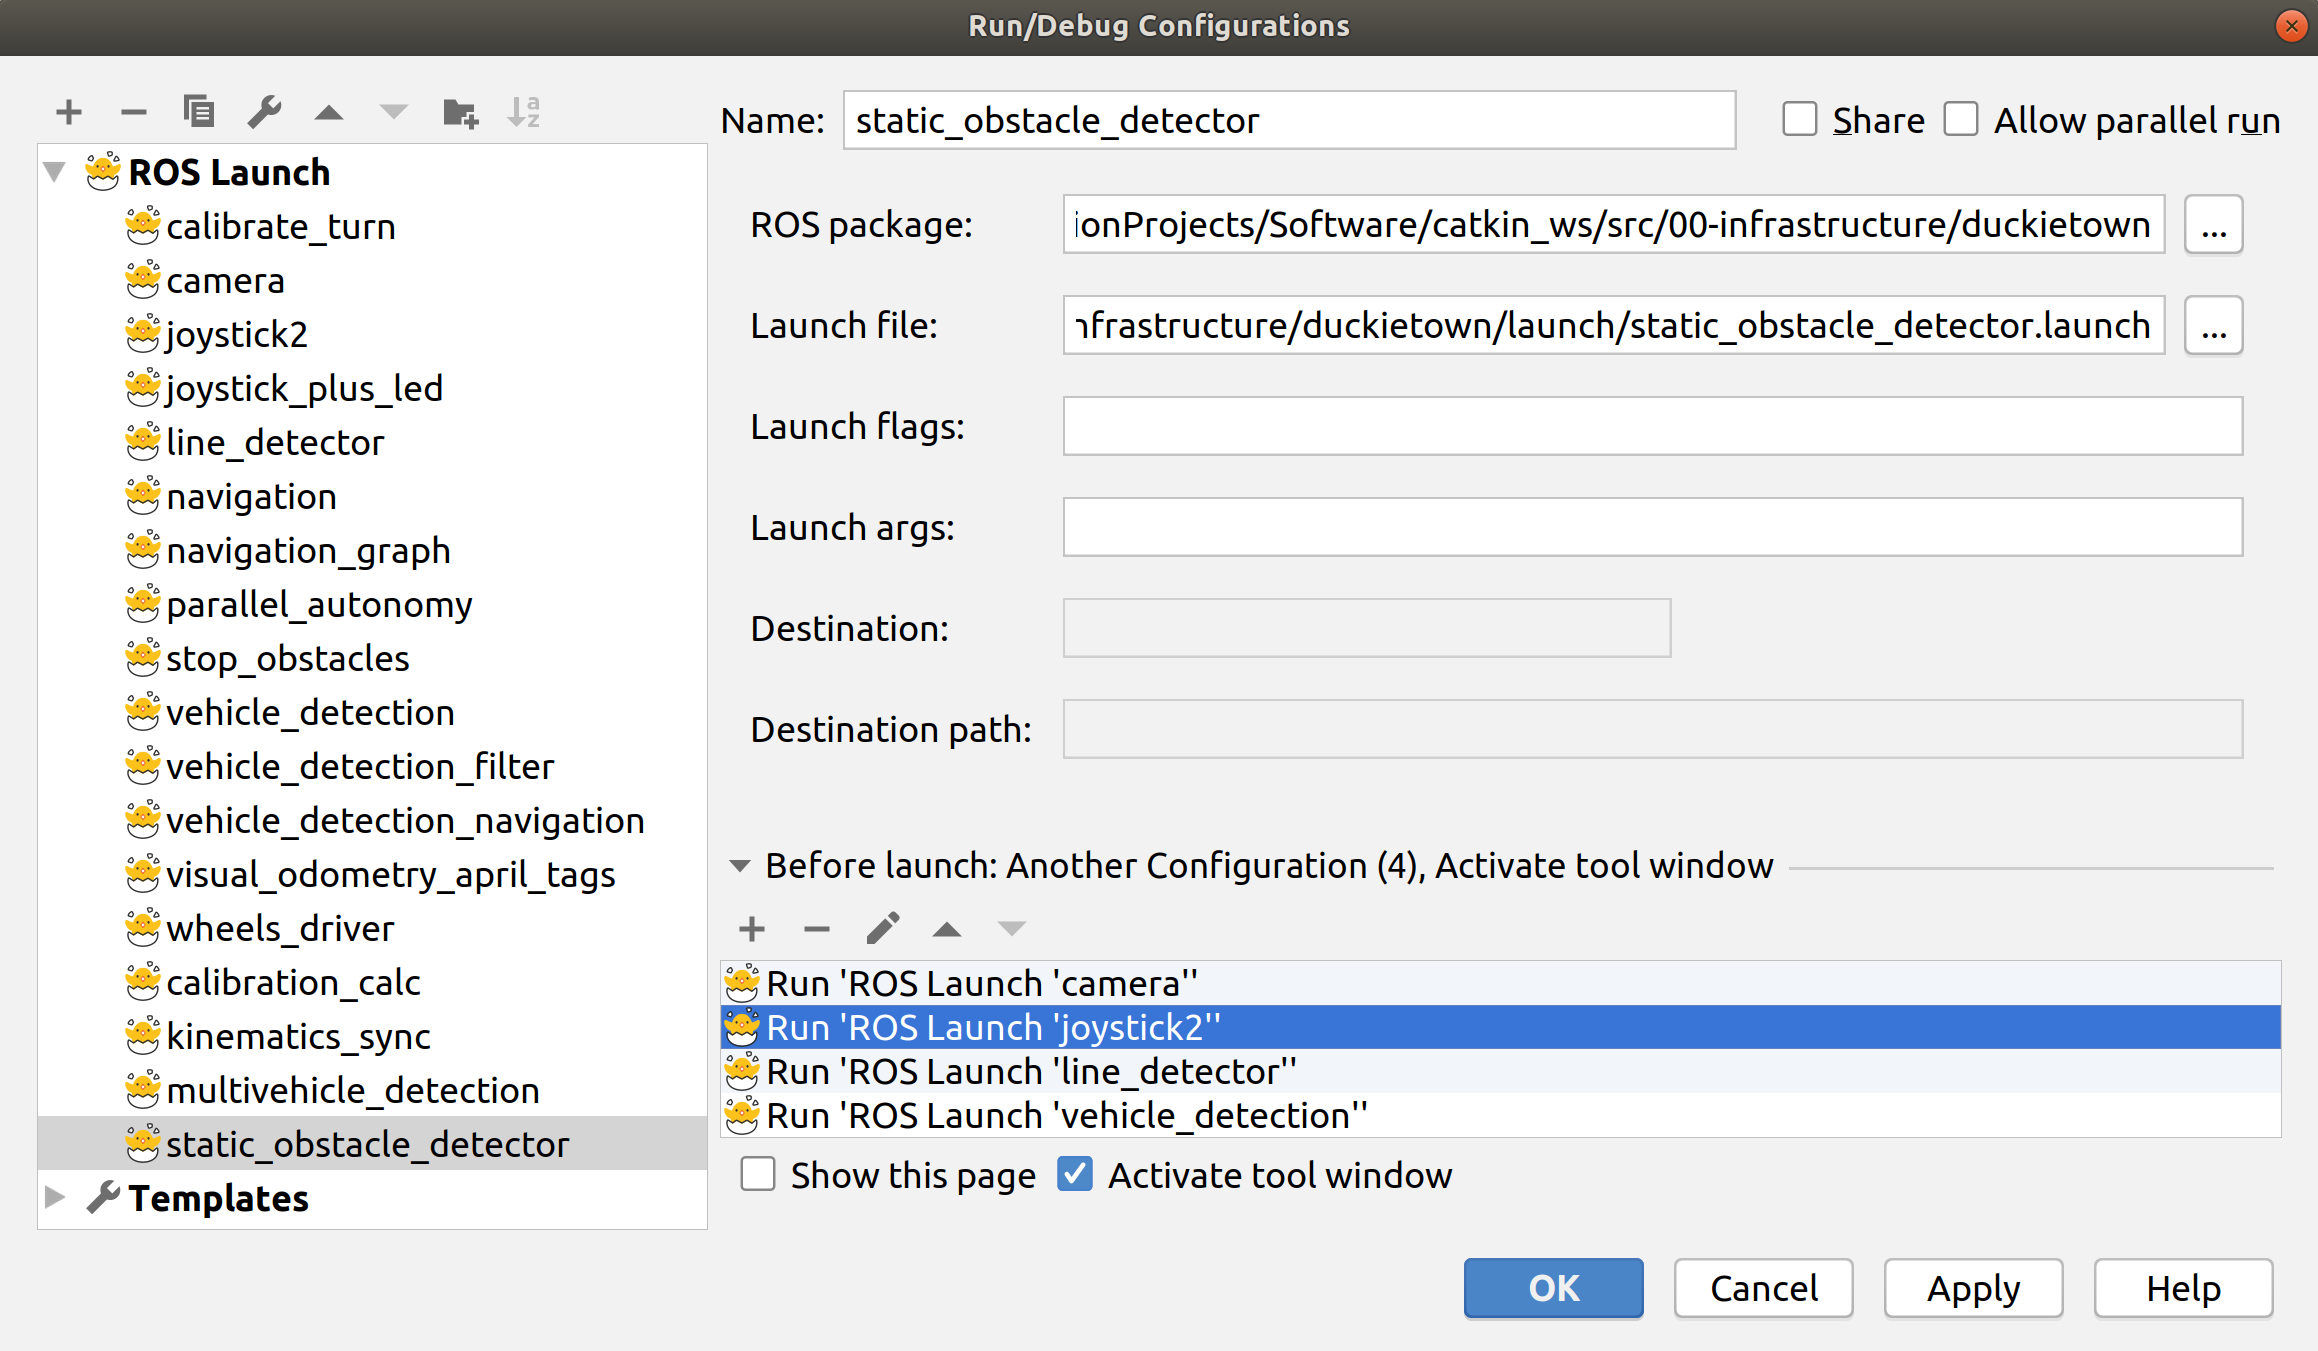
\includegraphics[width=0.90\textwidth]{ros_run_config.png}}
    \caption{Configuring a \inline{roslaunch} run configuration.}
    \label{fig:ros_run_config}
\end{figure}


\subsection{User interface}

An often overlooked, but important aspect of development tools is the user interface, being the primary mechanism through which developers edit source code. In the early days of modern computing, the only way of getting information into or out of a computer required punching holes in paper. Later, computers were equipped with technology to emit the same binary pattern as pixels, which could be used to display a small alphabet called ASCII. Later, through increased density and frequency, computers were able to render more sophisticated shapes and animations. This evolution is the direct result of advances in graphics technology, but can also be seen as progress in program representation, where the explicit source code was simply a medium for communicating developer intent and machine interpretation.

\begin{figure}
\centering
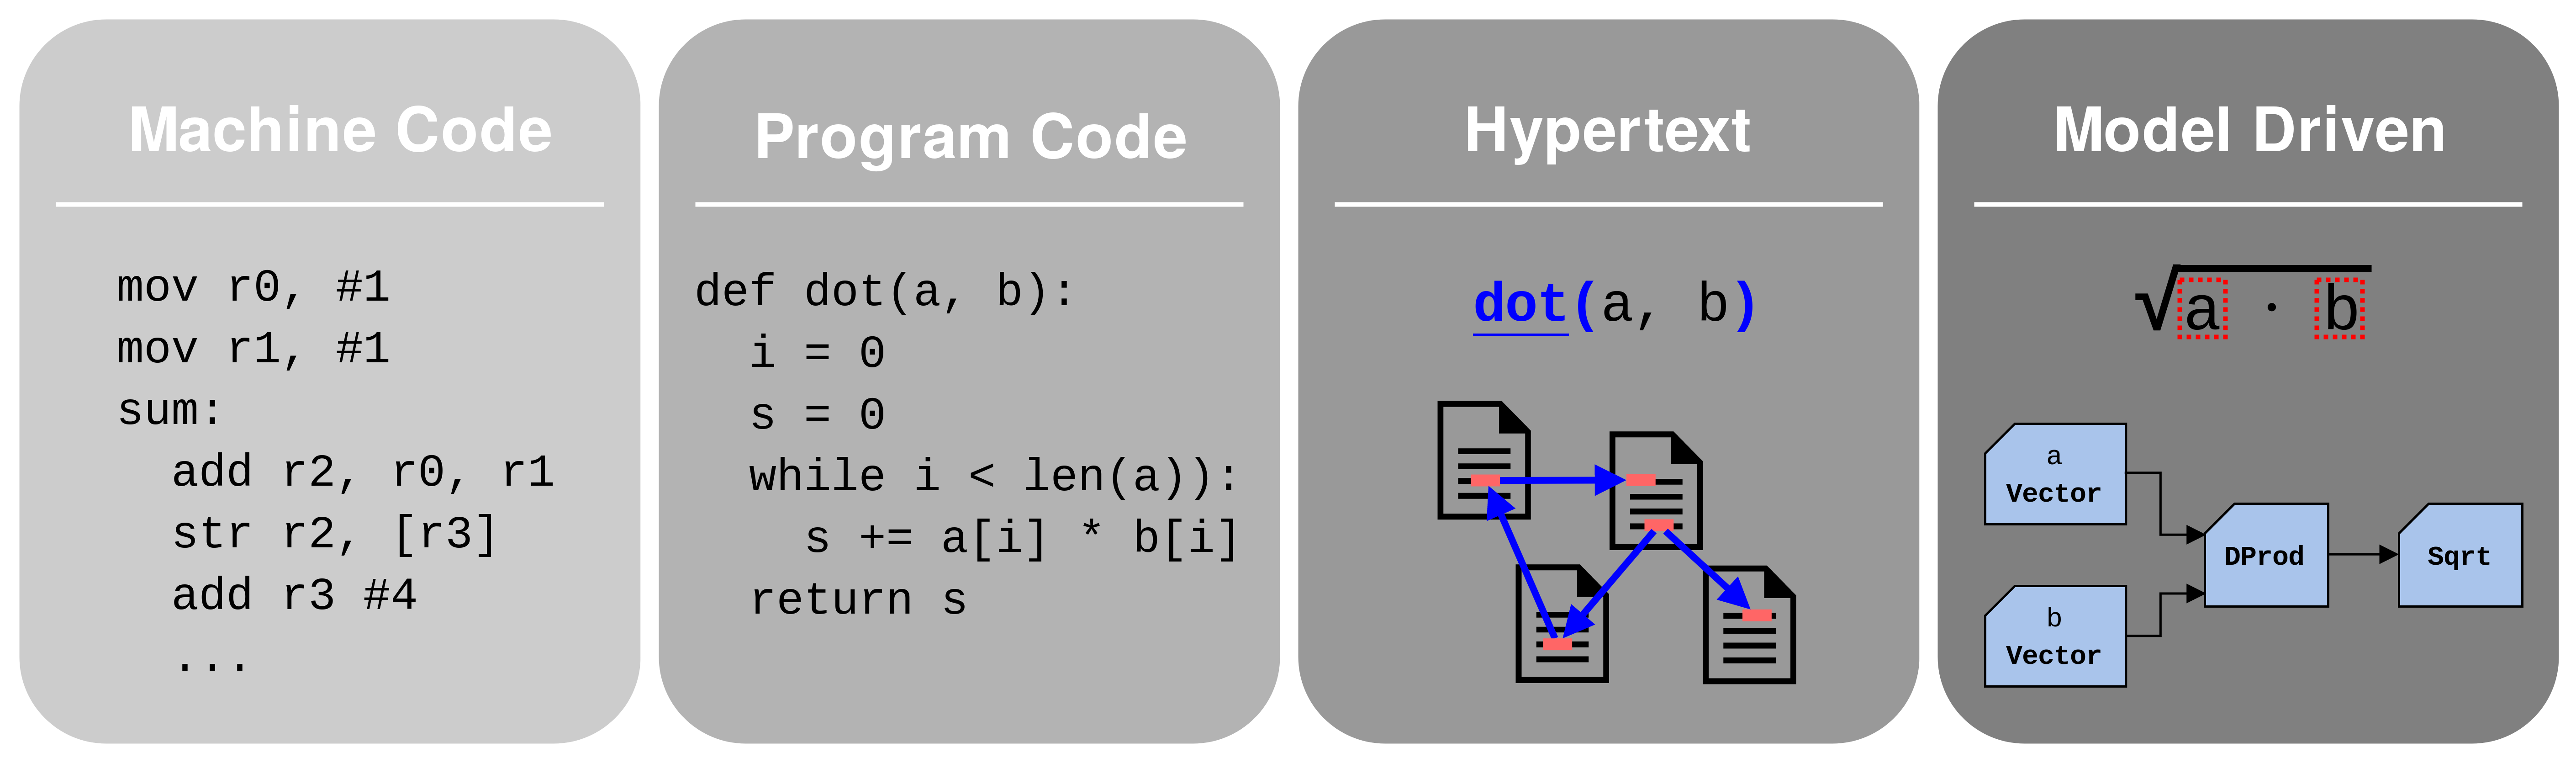
\includegraphics[width=0.90\textwidth]{progress_in_program.png}
\caption{The evolution of code. On the left are languages that force the user to adapt to the machine. To the right are increasingly flexible representations of source code.}
\label{fig:evolution_of_programming}
\end{figure}

ASCII is still the dominant medium for modern programming, although machines still use various forms of low level assembly code for execution. A great deal of software infrastructure is dedicated to translating between such representations via programming languages and compilers. While many developer tools provide a minimal command line interface (CLI), in addition to more sophisticated text editors for manipulating programs, these tools are still fairly restrictive. In the same way that early computer scientists probably did not fashion a new algorithm with a sequence of holes in mind, ASCII is also an indirect representation, albeit one slightly less contrived. Modern languages allow users to express their ideas in a notation is compact, familiar to use and easy to reason about its execution.

\begin{figure}
\centering
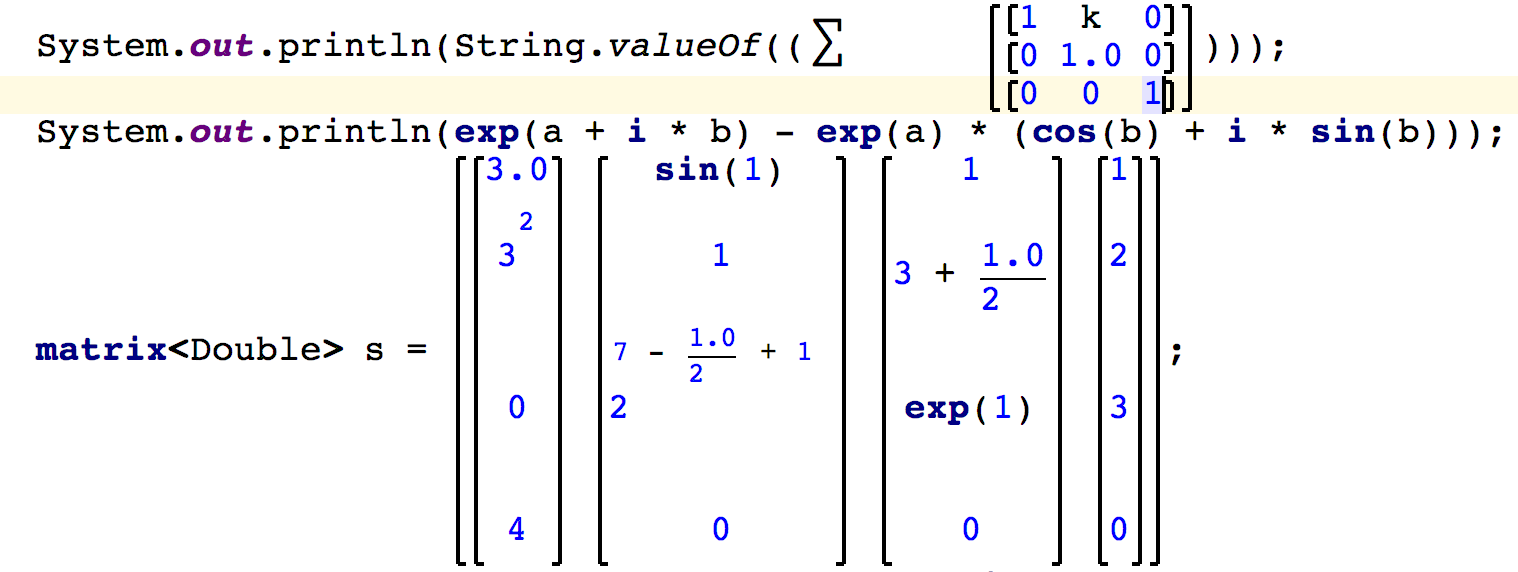
\includegraphics[width=0.90\textwidth]{mps_screenshot.png}
\caption{Projectional editors such as MPS~\citep{voelter2010language} (shown above)  are able to render plaintext source code in alternate formats for reading and manipulation.}
\label{fig:mps_screenshot}
\end{figure}

Modern programming tools are capable of representing code as a mixture of hypertext and graphical user interfaces. This provides a somewhat richer representation than plaintext and helps to capture programs' graph-based structure, but is rendered as ASCII with sparse visual cues. Some tools support larger character sets and font-based typographic ligatures, although the visual representation of source code remains highly linear.

More experimental UIs, such as model-driven engineering and \textit{projectional editors} offer more flexible visual layouts, through macro-based text replacement. This uncoupling between the composition and representation of text raises many intriguing questions. With the proliferation of new abstractions and programming shorthands, what is the appropriate level of notation required for a particular task? And who, or what, is the intended reader? These are important questions to ask when designing a developer tool.

In the case of Hatchery, we use a lightweight graphical user interface (GUI), most of which is provided by the underlying IDE platform. The plugin's primary job is to integrate smoothly with the IDE, which requires language- and framework-specific customizations.

\begin{figure}[b]
\centering
\frame{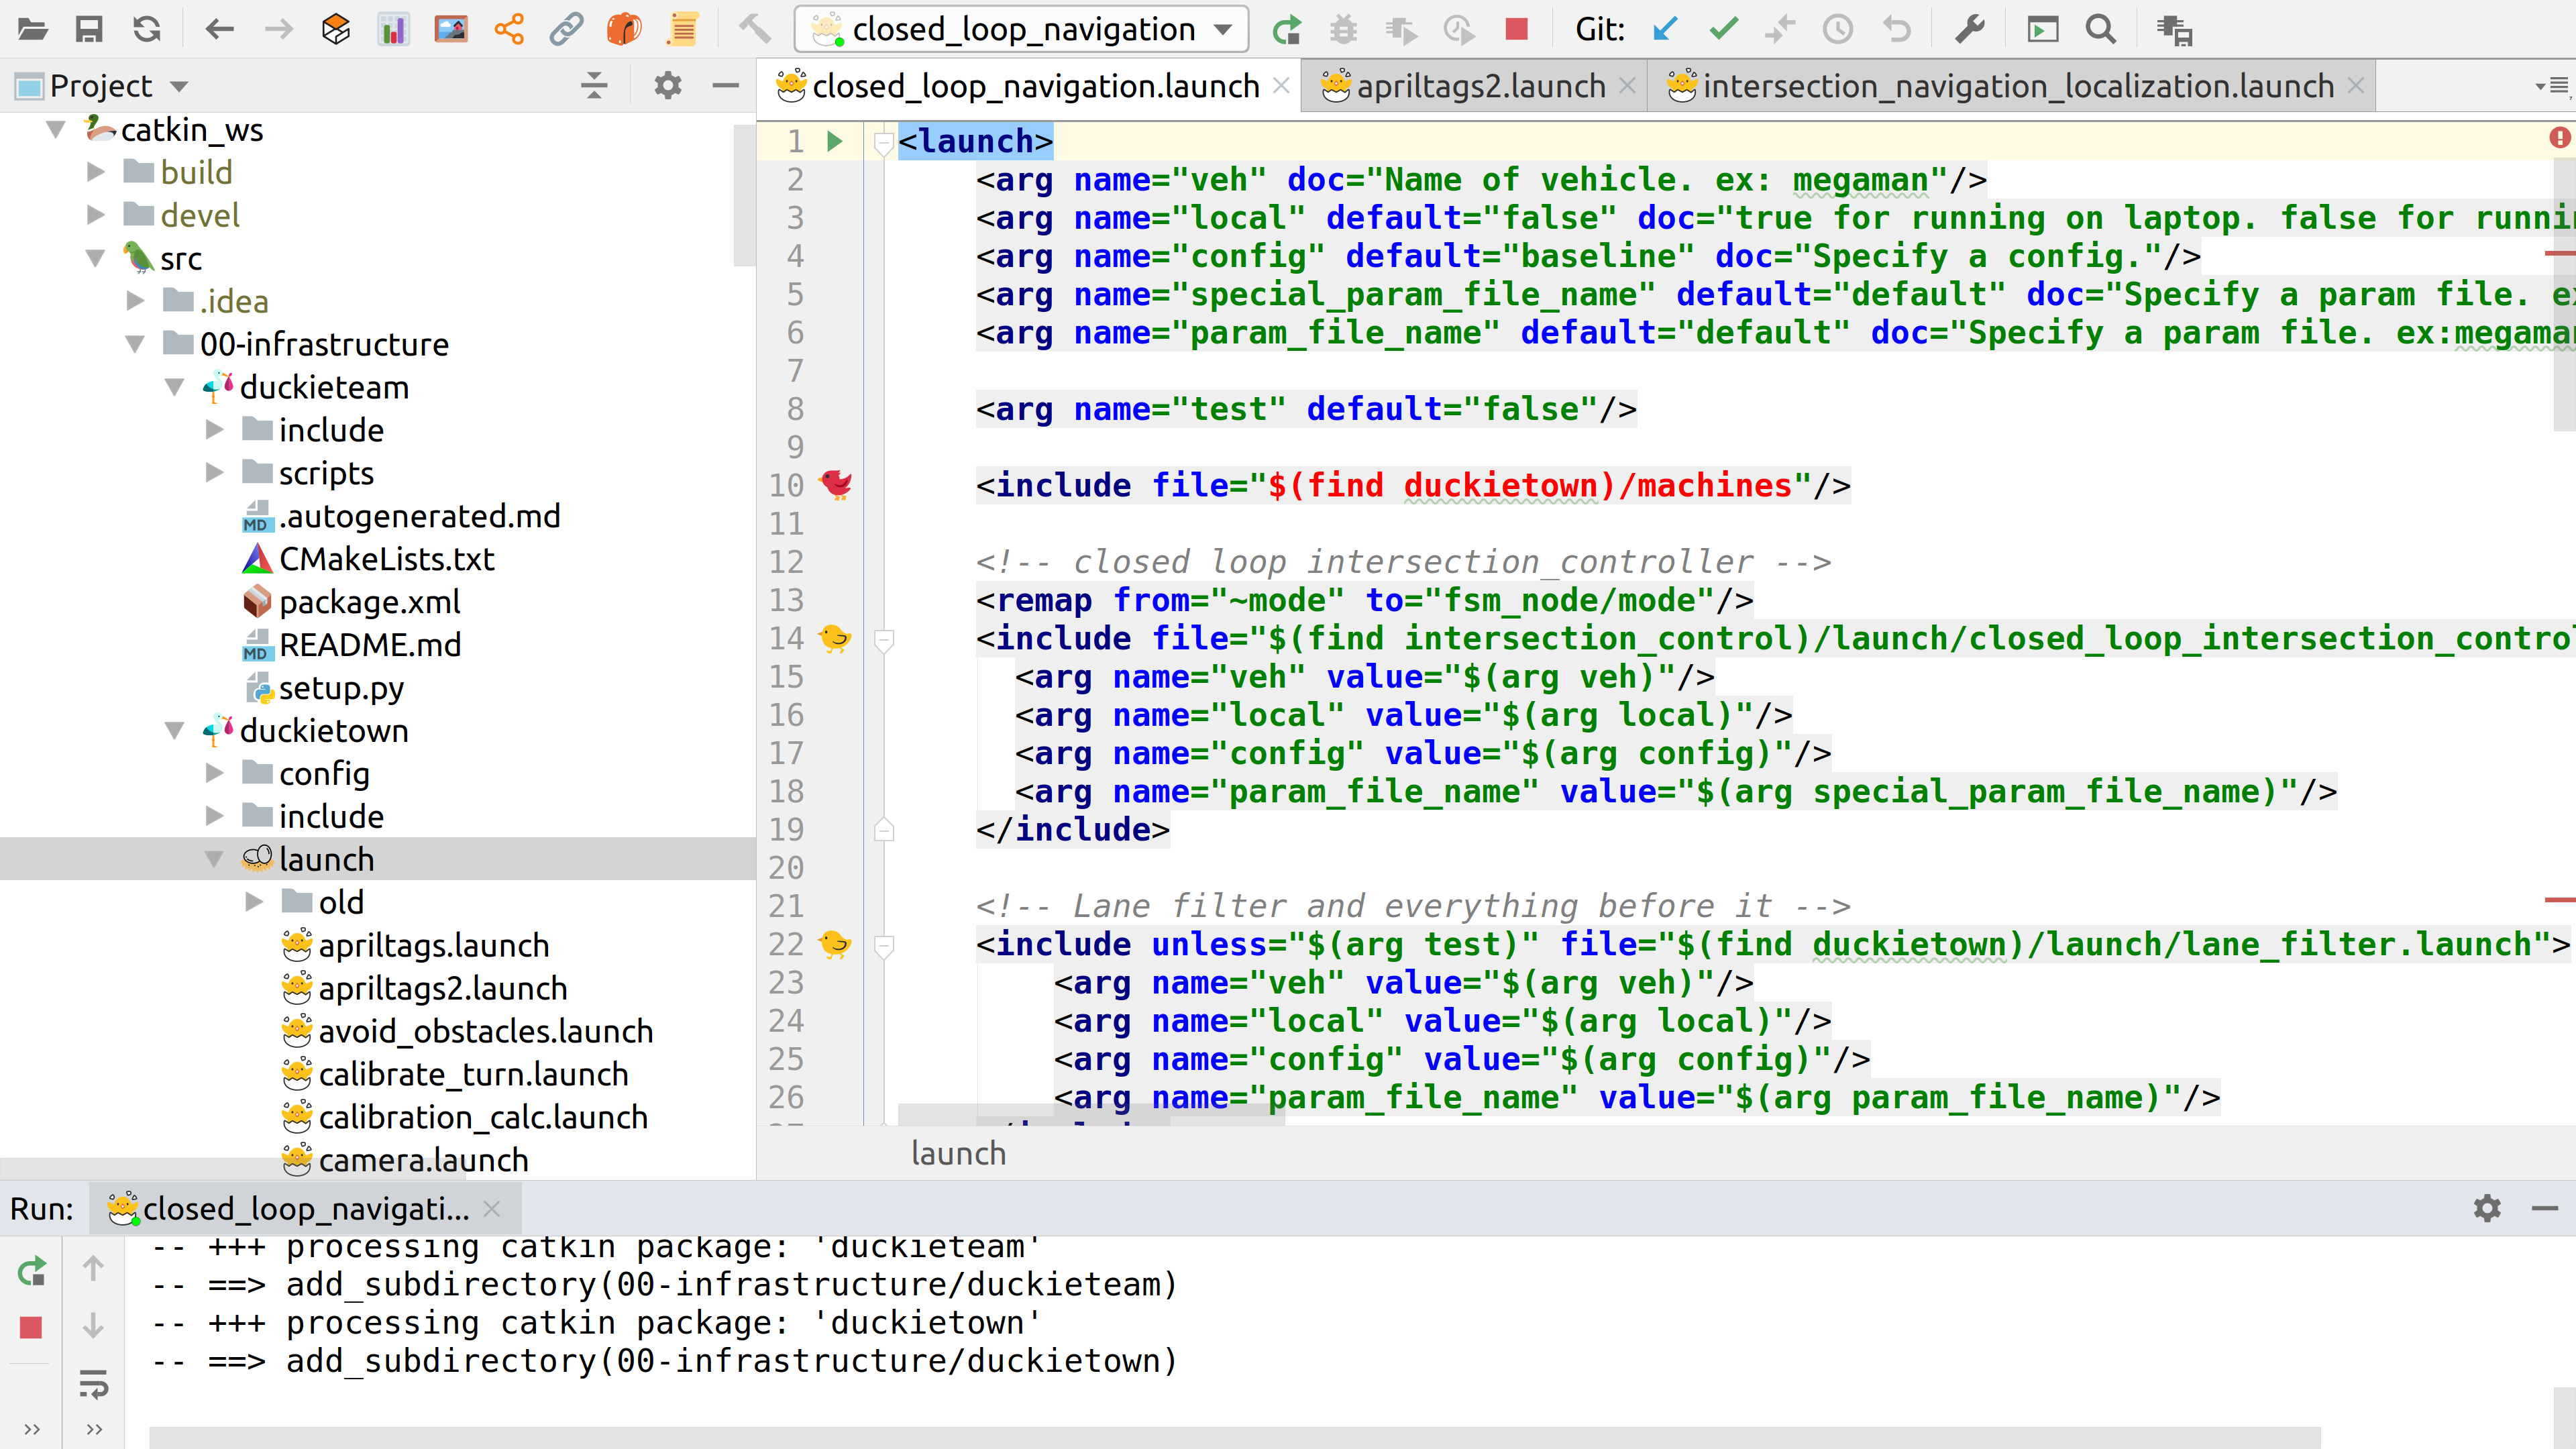
\includegraphics[width=0.90\textwidth]{hatchery_screenshot.png}}
\caption{Hatchery UI supports syntax highlighting, validation and project navigation.}
\label{fig:hatchery_gui}
\end{figure}

\begin{figure}
\centering
\frame{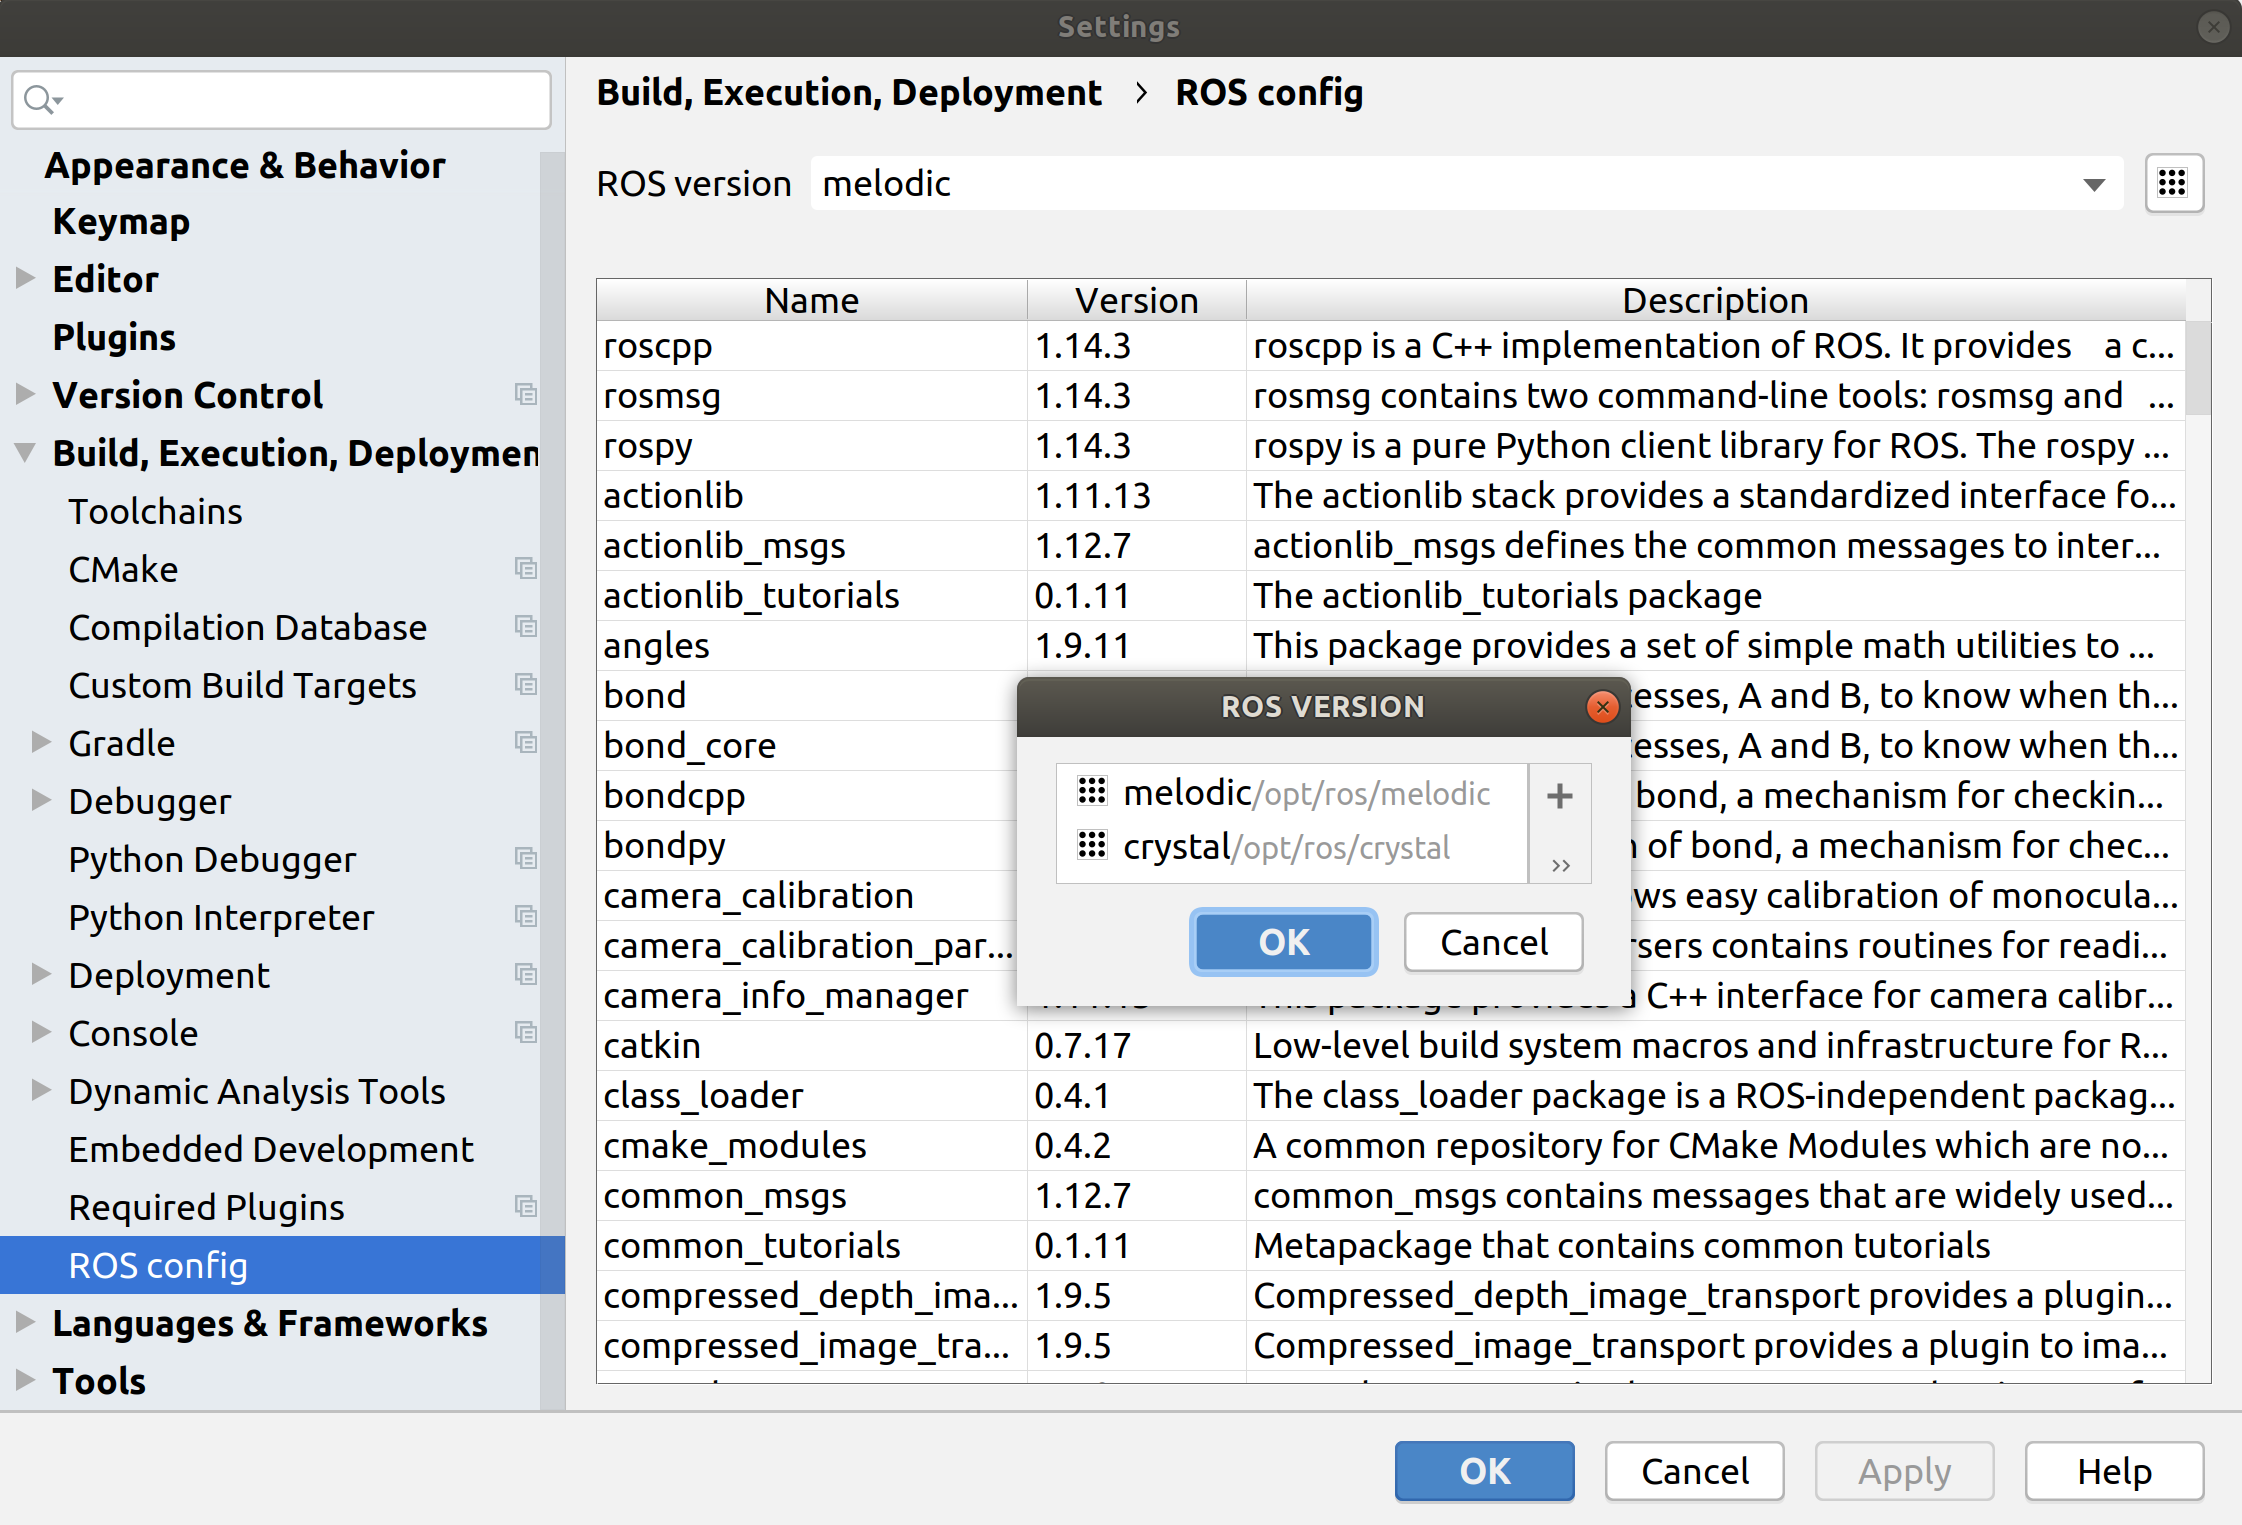
\includegraphics[width=0.90\textwidth]{ros_settings.png}}
\caption{Detection of local ROS packages.}
\label{fig:ros_settings}
\end{figure}

\section{Future work}

Detecting and managing ROS installations.

\welldone{\chapter{Implementation: languages and compilers}\label{ch:kotlingrad}}

\setlength{\epigraphwidth}{0.7\textwidth}
\epigraph{``The derivative, as this notion appears in the elementary differential calculus, is a familiar mathematical example of a function for which both [the domain and the range] consist of functions.''}{\begin{flushright}--Alonzo \citet{church1985calculi}, \textit{The Calculi of Lambda Conversion}\end{flushright}}

In this chapter, we will discuss the theory and implementation of a type safe domain-specific language for automatic differentiation (AD), which has produced a variety of applications in numerical optimization and machine learning. The key idea behind AD is fairly simple. A small set of primitive mathematical operations form the basis for all modern computers, and by composing these operations over the real numbers in an orderly fashion, one can compute any computable function. In machine learning, we are often given a computable function in the form of a program which does not work properly. We would like an algorithm for determining how to change the input slightly, so as to produce a more suitable output.

In 1964, such an algorithm was first conceived in~\citet{wengert1964simple}, whose method is known today as forward-mode AD. Not long after, a certain Richard Bellman reproduced Wengert's algorithm to numerically estimate the orbital dynamics of a two body system, recognizing its potential for, ``the treatment of large systems of differential equations which might not otherwise be undertaken''~\citep{bellman1965wengert}. Around the same time, key details of the backpropogation algorithm first emerged~\citep{dreyfus1990artificial}. It was in~\citet{linnainmaa1970representation} where the idea of calculating derivatives over computation graphs was first recorded. Linnaimaa's algorithm was particularly important for neural networks, and is today known as reverse-mode AD. But it was not until 2010 when standard software tools~\citep{bergstra2010theano} for AD became widely available in machine learning. It is here where our journey begins.

\section{Automatic differentiation}\label{sec:automatic-differentiation}

Given some input to a function, AD tells us how to change the input by a minimal amount, in order to maximally change the outputs. Suppose we are handed a function $P_k: \mathbb{R}\rightarrow\mathbb{R}$, composed of a series of nested functions, each with the same type:
%
\begin{equation}
    P_k(x) = \begin{cases} p_0(x) = x &\text{if } k=0\\ (p_k\circ P_{k-1})(x)&\text{if } k > 0 \end{cases}
\end{equation}
%
From the chain rule of calculus, we recall that:
%
\begin{equation}
    \frac{dP}{dp_0} = \frac{dp_k}{dp_{k-1}}\frac{dp_{k-1}}{dp_{k-2}}\dots\frac{dp_1}{dp_0}= {\displaystyle \prod_{i=1}^{k} \frac{dp_{i}}{dp_{i-1}}}
\end{equation}
%
Likewise, for a scalar function $Q(q_0, q_1, \dots, q_n):  \mathbb{R}^n\rightarrow\mathbb{R}$, the gradient $\nabla Q$ tells us:
%
\begin{equation}
    \nabla Q = \left( \frac{\partial Q}{\partial q_1}, \dots, \frac{\partial Q}{\partial q_n}\right)
\end{equation}
%
Occasionally, we may wish to compute the second-order partials for $Q$, i.e.\ the Hessian, $\mathbf{H}$:
%
\begin{equation}
\mathbf{H} = \begin{bmatrix}{\dfrac {\partial ^{2}Q}{\partial x_{1}^{2}}}&{\dfrac {\partial ^{2}Q}{\partial x_{1}\,\partial x_{2}}}&\cdots &{\dfrac {\partial ^{2}Q}{\partial x_{1}\,\partial x_{n}}}\\[2.2ex]{\dfrac {\partial ^{2}Q}{\partial x_{2}\,\partial x_{1}}}&{\dfrac {\partial ^{2}Q}{\partial x_{2}^{2}}}&\cdots &{\dfrac {\partial ^{2}Q}{\partial x_{2}\,\partial x_{n}}}\\[2.2ex]\vdots &\vdots &\ddots &\vdots \\[2.2ex]{\dfrac {\partial ^{2}Q}{\partial x_{n}\,\partial x_{1}}}&{\dfrac {\partial ^{2}Q}{\partial x_{n}\,\partial x_{2}}}&\cdots &{\dfrac {\partial ^{2}Q}{\partial x_{n}^{2}}}\end{bmatrix}
\end{equation}
%
More generally, for a vector function $\mathbf{f}:  \mathbb{R}^n\rightarrow\mathbb{R}^m$, the Jacobian $\mathbf J$ is defined as:
%
\begin{equation}
\mathbf J = \begin{bmatrix}
                       \dfrac{\partial \mathbf{f}}{\partial x_1} & \cdots & \dfrac{\partial \mathbf{f}}{\partial x_n} \end{bmatrix}
= \begin{bmatrix}
      \dfrac{\partial f_1}{\partial x_1} & \cdots & \dfrac{\partial f_1}{\partial x_n}\\
      \vdots & \ddots & \vdots\\
      \dfrac{\partial f_m}{\partial x_1} & \cdots & \dfrac{\partial f_m}{\partial x_n} \end{bmatrix}
    = \begin{bmatrix}
          \nabla f_1 \\
          \vdots \\
          \nabla f_n \end{bmatrix}
\end{equation}
%
For a vector function $\mathbf{P}_k(\mathbf{x}): \mathbb{R}^n\rightarrow\mathbb{R}^m$, the chain rule still applies:
%
\begin{align*}
\mathbf{J}_\mathbf{P_k} = \displaystyle \prod_{i=1}^{k} \mathbf{J}_{p_i} = \underbrace{\bigg(\Big((\mathbf{J}_{p_k} \mathbf{J}_{p_{k-1}}) \dots \mathbf{J}_{p_2}\Big) \mathbf{J}_{p_1}\bigg)}_{\textit{``Reverse accumulation''}} = \underbrace{\bigg(\mathbf{J}_{p_k} \Big(\mathbf{J}_{p_{k-1}} \dots (\mathbf{J}_{p_2} \mathbf{J}_{p_1})\Big)\bigg)}_{\textit{``Forward accumulation''}}
\end{align*}
%
For completeness, but rarely used in practice, is the second-order partials for vector functions:
%
\begin{equation}
\mathbf{H} (\mathbf {f} )=[\mathbf {H} (f_{1}), \mathbf {H} (f_{2}), \dots, \mathbf {H} (f_{m})]
\end{equation}
%
We can use these tools to compute the direction to adjust the inputs of a computable function, in order to maximally change that function's output, i.e.\ the direction of steepest descent.

\noindent Sometimes a function has the property that given an input $a$, no matter how $a$ is changed, the output remains the same. We say that such functions have zero gradient for that input.
%
\begin{equation}
    (\nabla F)(a) \approx \mathbf{0}
\end{equation}
%
The cost of calculating the Hessian, $\mathbf{H}$ is approximately quadratic~\citep{griewank1993some} with respect to the number of independent variables under differentiation. If $\mathbf{H}(a)$ is tractable to compute and invertible, we could use the second-partial derivative test to determine that:\\
%
\begin{enumerate}
    \item If all eigenvalues of $\mathbf{H}(a)$ are positive, $a$ is a local minimum
    \item If all eigenvalues of $\mathbf{H}(a)$ are negative, $a$ is a local maximum
    \item If $\mathbf{H}$ contains a mixture of positive and negative eigenvalues, $a$ is a \textit{saddle point}\\
\end{enumerate}
%
For some classes of computable functions, small changes to the input will produce a sudden large change in the output. We say that such functions are non-differentiable.
%
\begin{equation}
    ||\nabla F|| \approx \pm \infty
\end{equation}
%
It is an open question whether non-differentiable functions exist in the real world~\citep{buniy2005hilbert}. At the current physical (10nm) and temporal (10ns) scale of modern computing, there exist no such functions, but most modern computers are incapable of reporting the true value of their binary-valued functions. For all intents and purposes, programs implemented by most physical computers are discrete relations. Nevertheless, discrete programs are capable of approximating bounded functions of $\mathbb{R}^n$ to arbitrary precision given enough time and space. For most applications, a low precision (32-64 bit) approximation is sufficient.

There exists at the heart of machine learning a theorem that states a simple family of functions, which compute a weighted sum of a non-linear function $\varphi: \mathbb{R} \rightarrow \mathbb{R}$ composed with a linear function $\theta^\intercal x + b$, can approximate any bounded function on $\mathbb{R}^m$ to arbitrary precision. More precisely, the universal approximation theorem~\citep{hornik1989multilayer} states that for all real-valued continuous functions $\mathbf{f}: C(\mathbb{I}_m)$, where $\mathbb{I}_m = [0, 1]^m$, there exists a function $\mathbf{\hat f}$, parameterized by constants $n \in \mathbb{N}, \mathbf{\beta} \in \mathbb{R}^n, \mathbf{b} \in \mathbb{R}^n, \epsilon \in \mathbb{R}^+$ and $\mathbf{\theta} \in \mathbb{R}^{m \times n}$:
%
\begin{equation}
    \begin{split}
        \mathbf{\hat{f}}(\mathbf{x}) = \mathbf{\beta}^\intercal \varphi_{\odot} \left(\mathbf{\theta}^\intercal \mathbf{x} + \mathbf{b}\right) \\
        \forall \mathbf{x} \in \mathbb{I}_m, \ | \mathbf{\hat f}( \mathbf{x} ) - \mathbf{f} ( \mathbf{x} ) | < \epsilon
    \end{split}
\end{equation}
%
This theorem does not provide any method for how to find $\theta$ nor does it place an upper bound on the constant $n$, somewhat limiting its practical applicability. But for reasons not yet fully understood, empirical results suggest it is possible to approximate many naturally-arising functions in a relatively short time by composing several \textit{layers} of $\mathbf{\theta}^\intercal \mathbf{x} + \mathbf{b}$ and $\varphi$ in an alternating fashion. The resulting model might be expressed as,
%
\begin{equation} \label{eq:recursive_parametric_eq}
    \mathbf{\hat P}_k(\mathbf{x}; \mathbf{\Theta}) = \begin{cases} \mathbf{\hat p}_0(\mathbf\theta_0)(\mathbf{x}) &\text{if } k=0\\ \big(\mathbf{\hat p}_k(\mathbf\theta_k)\circ \mathbf{\hat P}_{k-1}(\mathbf{\Theta}_{[0, k-1]})\big)\big(\mathbf{x}\big)&\text{if } k > 0 \end{cases} \\
\end{equation}
%
where $\mathbf\Theta = \{\mathbf\theta_0, \dots, \mathbf\theta_k\}$ are free parameters and $\mathbf{x} \in \mathbb{R}^n$ is a single input. To approximate $\mathbf{P}(\mathbf x)$, one must obtain $\mathbf{X} = \{\mathbf{x}^{(0)}, \dots, \mathbf{x}^{(z)}\}, \mathbf{Y} = \{\mathbf{y}^{(0)} = \mathbf{P}(\mathbf{x}^{(0)}), \dots, \mathbf{y}^{(z)} = \mathbf{P}(\mathbf{x}^{(z)})\}$ in as great and varied a quantity as possible and repeat the following procedure until $\mathbf\Theta$ converges:
%
\begin{equation} \label{eq:stochastic_grad_descent}
    \mathbf\Theta \leftarrow \mathbf\Theta - \alpha\frac{1}{z}\nabla_{\mathbf\Theta} \sum_{i=0}^z\mathcal{L}\big(\mathbf{\hat P}_k(\mathbf{x}^{(i)}; \mathbf{\Theta}), \mathbf{y}^{(i)}\big)
\end{equation}
%
For most common $\mathcal{L}$, the complexity of this procedure is linear with $z$. As $z$ can be quite large in practice, and since obtaining the exact gradient is not very important, we use a stochastic variant by randomly resampling a \textit{minibatch} $\mathbf{X}', \mathbf{Y}'$ consisting of pairs $\mathbf{x}^{(i)}, \mathbf{y}^{(i)}$ for $i \sim \{0..z\}$ on each update. This is slightly noisier, but runs considerably more quickly.

\section{Differentiable programming}\label{sec:differentiable-programming}

\begin{figure}
    \centering
    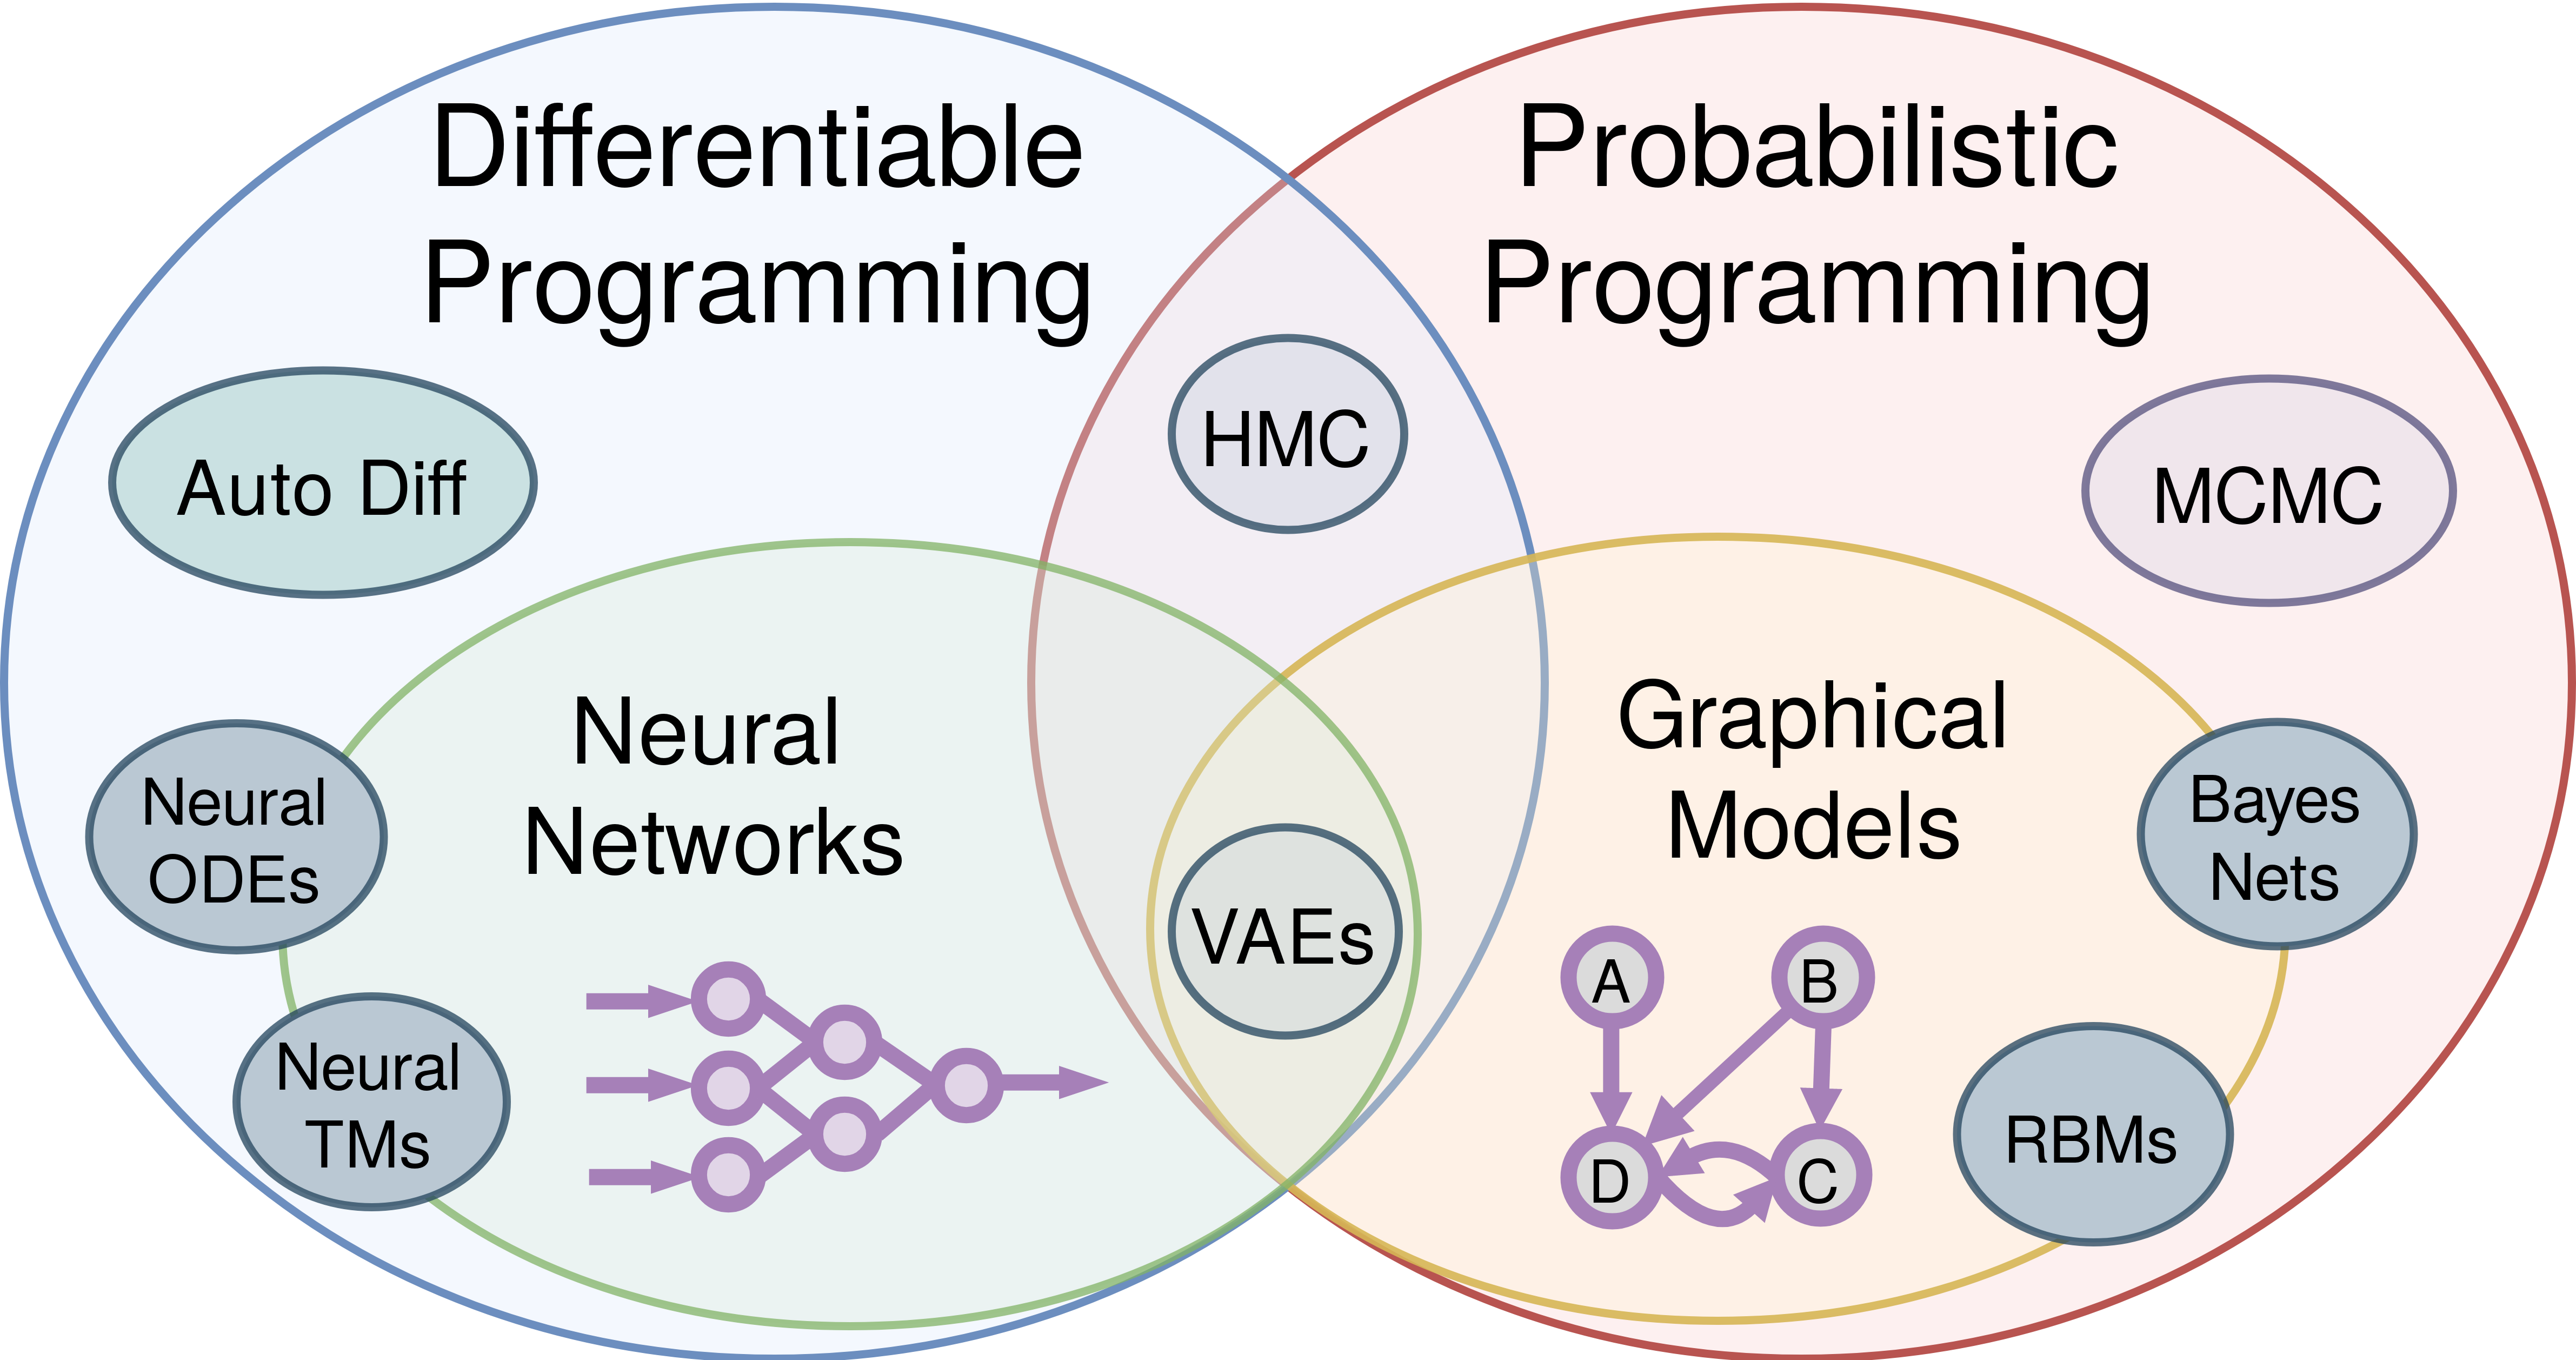
\includegraphics[width=0.90\textwidth]{diff_prob_prog.png}
    \caption{\textit{Differentiable programming} includes neural networks, but more broadly, arbitrary differentiable programs which use automatic differentiation and gradient-based optimization to approximate a loss function. \textit{Probabilistic programming} is a generalization of probabilistic graphical models, and uses various forms of Markov chain Monte Carlo (MCMC) and differentiable inference to approximate a probability density function.}
    \label{fig:diff_prob_prog}
\end{figure}

The renaissance of modern deep learning is widely attributed to progress in three research areas: algorithms, data and hardware. Among algorithms, most research has focused on deep learning architectures and representation learning. Equally important, arguably, is the role that automatic differentiation (AD) has played in facilitating the implementation of these ideas. Prior to the adoption of general-purpose AD libraries such as Theano, PyTorch and TensorFlow, gradients had to be derived manually. The widespread adoption of AD software simplified and accelerated the pace of gradient-based machine learning, allowing researchers to build deeper network architectures and new learning representations. Some of these ideas in turn, formed the basis for new methods in AD, which continues to be an active area of research in the programming language community.

A key aspect of the connectionist paradigm is gradient descent on a statistical loss function with respect to the free parameters of a neural network. For gradient descent to work, the representation must be differentiable almost everywhere. However many representations are non-differentiable in their natural domain. For example, the structure of language in its written form is not easily differentiable, as small changes to a word's symbolic representation can cause sudden changes to its semantic meaning. A key insight from representation learning is that many discrete data types can be mapped to a smoother latent space. For example, if we represent words as a vector of real numbers, then it is possible to learn a mapping from the textual domain to the vector representation so that the semantic relations between words (as measured by their statistical co-occurrence in large language corpora) are geometrically preserved in vector space~\citep{pennington2014glove} -- words with similar meanings map to similar vectors. It so happens that many classes of discrete problems can be relaxed to continuous surrogates by learning such representations, or \textit{embeddings} in an unsupervised, or semi-supervised manner.

Around the same time, the deep learning community realized that perhaps strict differentiability was not so important all along. It was shown in practice, that computers using low-precision arithmetic such as 8-bit floating point~\citep{wang2018training} and integer~\citep{jacob2018quantization} quantization are able to train neural networks without sacrificing performance. Strong assumptions like Lipschitz-continuity and $\beta$-smoothness once thought to be indispensable for gradient-based learning could be relaxed, as long as the noise introduced by quantization was negligible compared to stochastic gradient methods. In hindsight, this should have been less surprising, since all digital computers use discrete representations anyway and were capable of training neural networks for nearly half a century. This suggests strict differentiability was not as important as having a good metric. As long as the loss surface permits metric learning, gradient descent is surprisingly resilient to quantization.

As deep learning solved problems across various domains, researchers observed that neural networks were part of a broader class of differentiable architectures that could be designed, implemented and analyzed in a manner not unlike computer programs. Hence the term \textit{differentiable programming} (DP) was born. Today, DP has found a wide range of applications, from protein folding~\citep{alquraishi2018end}, to physics engines~\citep{de2018end,DBLP:journals_corr_DegraveHDW16} and graphics rendering~\citep{loper2014opendr} to meta-learning~\citep{liu2018darts}. These domains have well-studied dynamics models, with parameters that can be tuned via gradient descent. Traditionally, handcrafted optimization algorithms were required to learn these parameters, but given a smooth metric, DP promises to do this for a broad class of models, more or less automatically. For discrete optimization however, DP is not sufficient. To automatically learn discrete relations without ad hoc embedding, additional tools, such as probabilistic programming, are likely needed. As seen in \autoref{fig:diff_prob_prog}, these two fields have developed many productive collaborations in recent years.

\section{Static and dynamic languages}

Most programs in machine learning and scientific computing are written in dynamic languages, such as Python. In contrast, most of the industry uses statically typed languages~\citep{github}. According to some studies, type related errors account for over 15\% of software bugs~\citep{gao2017type}. While the causality on using static typing and fewer defects has not been conclusively established, dynamically typed languages are seldom used for building safety-critical systems, and the majority of robotics applications~\citep{Areserio54:online} are written in statically typed languages.

Statically typed languages eliminate a broad class of runtime errors and allow users to reason about the behavior of programs without needing to execute them. In addition to stronger syntax validation for general purpose programming, a well-designed library in a strongly typed language can eliminate specific errors related to API misuse that would otherwise require documentation and code samples to prevent, reducing the burden of discovery and maintenance. Furthermore, strong type systems enable more powerful static analysis tools, which can provide relevant autocompletion, source code navigation, and earlier detection of runtime errors.

One frequent objection to using strongly typed languages is attributed to the additional burden of manual type annotation. While early type-safe languages like C/C++ and Java required programmers to exhaustively annotate function and variable declarations, with judicious use of type inference in modern languages like Kotlin, Scala, Rust et al., most type signatures may be safely omitted and easily recovered from the surrounding context. Type inference enables modern languages to offer the brevity of dynamically typed languages with the safety of static type checking.

\section{Imperative and functional languages}

Most programs written today are written in the imperative style, due the prevalence of the Turing Machine and von Neumann architecture~\citep{backus2007can}. $\lambda$-calculus provides an equivalent\footnote{In the sense that the Turing Machine and $\lambda$-calculus are both Turing Complete.} language for computing, which we argue, is a more appropriate notation for expressing mathematical functions and computing their derivatives. In imperative programming the sole purpose of using a function is to pass it values, and there is no way to refer to a function directly. More troubling in the case of AD, is imperative programs have mutable state, which requires taking extra precautions when computing their derivatives.

The mathematical notion of function composition is a first-class citizen in functional programming. Just as we do in calculus, to take the derivative of a program composed with another program, simply apply the chain rule (cf.~\autoref{sec:automatic-differentiation}). Since there is no mutable state in FP, no exotic data structures or compiler tricks are required.

For example, consider the vector function $f(l_1, l_2) = l_1 \cdot l_2$, seen in \autoref{fig:fp_vs_ip}. Imperative programs, by allowing mutation, are destroying intermediate information. In order to recover the computation graph for reverse mode AD, we either need to override the assignment operator, or use a tape to store the intermediate values, which is quite tedious. In pure functional programming, mutable variables do not exist, which makes our lives much easier.

\begin{figure}[t]
    \centering
    \begin{tabular}{|l|l|}
        \hline
        Imperative & Functional \\
        \hline
        {\begin{lstlisting}[style=barelisting, linewidth=5.5cm, numbers=left]
fun dot(l1, l2) {
  if (len(l1) != len(l2))
    return error
  var sum = 0
  for(i in 0 to len(l1))
    sum += l1[i] * l2[i]
  return sum
}
        \end{lstlisting}}
         &
        {\begin{lstlisting}[style=barelisting, linewidth=5.5cm, numbers=none]
fun dot(l1, l2) {
  return if (len(l1) != len(l2))
    error
  else if (len(l1) == 0) 0
  else
    head(l1) * head(l2) +
    dot(tail(l1), tail(l2))
}
        \end{lstlisting}}
        \\
        \hline
    \end{tabular}
    \caption{Two equivalent programs, both implementing the function $f(l_1, l_2) = l_1 \cdot l_2$.}
    \label{fig:fp_vs_ip}
\end{figure}

Kotlin$\nabla$ treats mathematical functions and programming functions with the same underlying abstraction. Expressions are composed to form a data-flow graph (DFG). An expression is simply a \inline{Function}, which is only evaluated when invoked with numerical values, e.g. \inline{z(0, 0)}. In this way, Kotlin$\nabla$ is similar to other compiled graph-based approaches like TensorFlow and Theano.

\section{Kotlin}\label{sec:kotlin}

When programming in a statically typed language, a common question one might ask the compiler is, ``Given a value, \inline{x}, can \inline{x} be assigned to a variable of type \inline{Y}?'' (e.g. type checking\inline{x instanceof Y}) In Java, this question turns out to be unsound~\citep{amin2016java} and undecidable~\citep{Grigore:2017:JGT:3009837.3009871} in the general case. It is possible to construct a Java program in which the answer is ``yes'' regardless of \inline{Y}, or for which the answer cannot be determined in a finite amount of time. In the latter case, this is not necessarily a problem, but the former case is more critical and unclear how to fix, even if it rarely occurs in practice.

Kotlin is a strong, statically typed language, that is well-suited for building cross-platform applications, targeting JVM, JavaScript and native. Unlike most programming languages, the language was designed with IDE support from the outset, and owes much of its popularity to its programming ergonomics. Kotlin's type system~\citep{tate2013mixed} is strictly less expressive, but fully interoperable with Java's. It is unknown whether the the same issues which affect Java's type system are present in Kotlin's, but interoperability with Java spurred its adoption and remains a key usability feature of the language.

In this work, we make use of several language features unique to Kotlin, such as first-class functions (\autoref{sec:first-class-functions}), extension functions (\autoref{sec:extension-functions}), operator overloading (\autoref{sec:operator-overloading}), and algebraic data types (\autoref{sec:adts}). Furthermore, we make heavy use of Kotlin's DSL support for shape-safe array programming. Together, these language features provide a concise, flexible and type-safe platform for mathematical programming.

\section{Kotlin$\nabla$}\label{sec:kotlingrad}

Prior work has shown it is possible to encode a deterministic context-free grammar as a \textit{fluent interface}~\citep{gil2016formal} in Java. This result was strengthened to prove Java's type system is Turing complete~\citep{Grigore:2017:JGT:3009837.3009871}. As a practical consequence, we can use the same technique to perform shape-safe automatic differentiation (AD) in Java, using type-level programming. A similar technique is feasible in any language with generic types.

Differentiable programming has a rich history among dynamic languages like Python, Lua and JavaScript, with early implementations including projects like Theano~\citep{theano}, Torch~\citep{collobert2002torch}, and TensorFlow~\citep{abadi2016tensorflow}. Similar ideas have been implemented in statically typed, functional languages, such as Haskell's Stalin$\nabla$~\citep{pearlmutter2008using}, DiffSharp in F\#~\citep{baydin-diffsharp} and recently Swift~\citep{swift}. However, the majority of existing automatic differentiation (AD) libraries use a loosely-typed DSL, and few offer shape-safe tensor operations in a widely-used programming language.

Existing AD implementations for the JVM include Lantern \citep{wang2018demystifying}, Nexus \citep{chen2017typesafe} and DeepLearning.scala~\citep{dl4s}, however these are Scala-based and do not interoperate with other JVM languages. Kotlin$\nabla$ is fully interoperable with vanilla Java, enabling broader adoption in neighboring languages. To our knowledge, Kotlin has no prior AD implementation. However, the language has several useful features for implementing a native AD framework. Kotlin$\nabla$ primarily relies on the following language features:

\begin{itemize}
\item \textbf{Operator overloading and infix functions} allow a concise notation for defining arithmetic operations on tensor-algebraic structures, i.e.\ groups, rings and fields.
\item \textbf{$\mathbf{\lambda}$-functions} support functional programming, following~\citet{pearlmutter2008reverse, pearlmutter2008using, siskind2008nesting, elliott2009beautiful, elliott2018simple}, et al.
\item \textbf{Extension functions} support extending classes with new fields and methods which can be exposed to external callers without requiring sub-classing or inheritance.
\end{itemize}

\begin{figure}
    \centering
    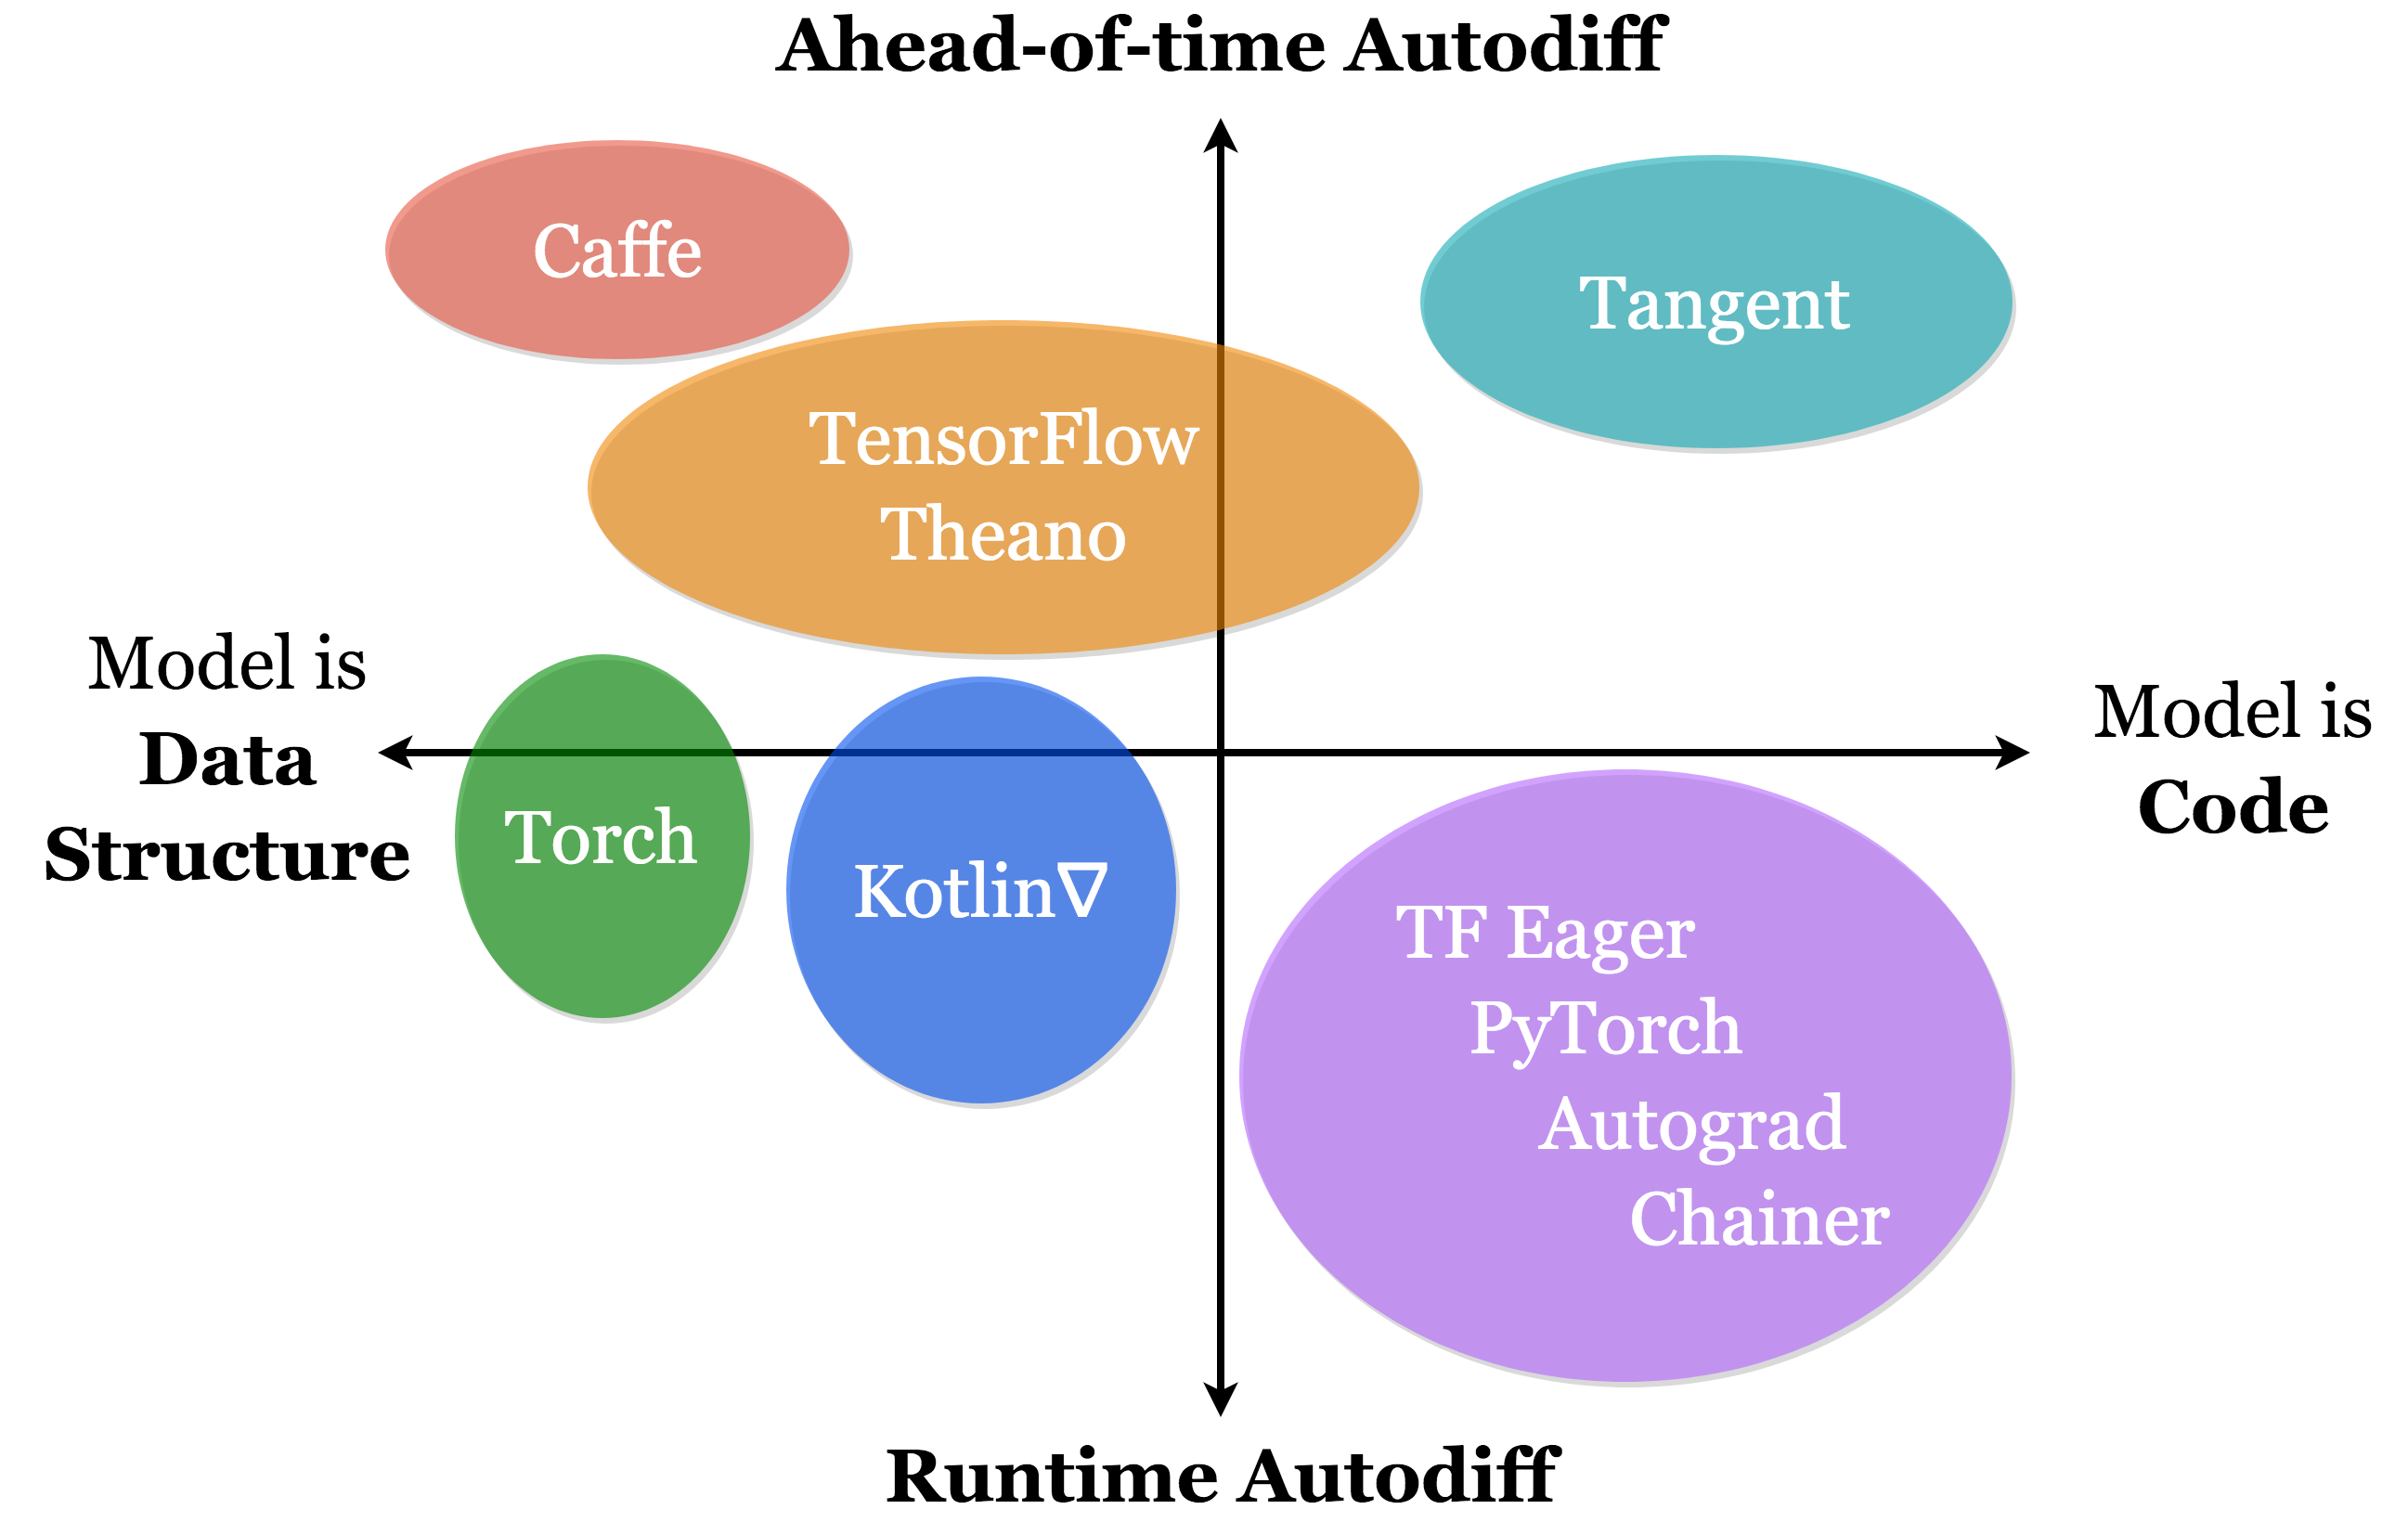
\includegraphics[width=0.70\textwidth]{kotlingrad_diagram.png}
    \caption{Adapted from~\citet{van2018tangent}. Kotlin$\nabla$ models are data structures, constructed by an embedded DSL, eagerly optimized, and lazily evaluated at runtime.}
    \label{fig:kotlingrad_digram}
\end{figure}

Kotlin$\nabla$ models are embedded domain-specific languages (eDSLs), which are essentially data structures masquerading as code. These structures may look and act like code, but are really just functions for building an abstract syntax tree (AST), which can be evaluated eagerly or lazily depending on the user's needs. Typically these ASTs represent simple state machines, but they can also be used to implement a full-fledged programming language. Popular examples include SQL/LINQ~\citep{meijer2006linq}, OptiML~\citep{sujeeth2011optiml} and other fluent interfaces~\citep{fowler05fluent}. In a sufficiently expressive host language, one can implement any language as a library, without needing to write a lexer, parser, compiler or interpreter. And with a carefully designed type system, users will automatically receive code completion and static analysis from their favorite developer tools. Many have observed that functional programming languages are suitable host languages~\citep{elliott2003compiling,rompf2010lightweight}, perhaps owing to the notion of code as data.\footnote{i.e.\ homoiconicity, notably introduced by Lisp, one of the first functional programming languages}

\section{Usage}

Kotlin$\nabla$ allows users to implement differentiable programs by composing expressions. Consider the following Kotlin$\nabla$ program with two inputs and one output:
%
\begin{figure}[H] \label{fig:basic_kotlingrad}
\begin{unbreakablelisting}[caption={, rendered below.}]
with(DoublePrecision) { // Uses double precision numerics for evaluation
  val x = Var("x") // Declare immutable variables (these variables are
  val y = Var("y") // just symbolic constructs used for differentiation)
  val z = sin(10 * (x * x + pow(y, 2))) / 10 // Lazily evaluated
  val dz_dx = d(z) / d(x) // Supports Leibniz's notation
  val d2z_dxdy = d(dz_dx) / d(y) // Mixing higher order partials
  val d3z_d2xdy = grad(d2z_dxdy)[x] // Equivalent to d(f)/d(x)
  plot3D(d3z_d2xdy, -1.0, 1.0) // Plot in 3-space (-1 < x, y, z < 1)
}
\end{unbreakablelisting}
%    \centering $z = \sin{\big(10(x*x + y^2)\big)} / 10$, \texttt{plot}$\Big\left(\frac{\partial^{3z}}{\partial{x^2}\partial{y}}\Big\right)$ \\
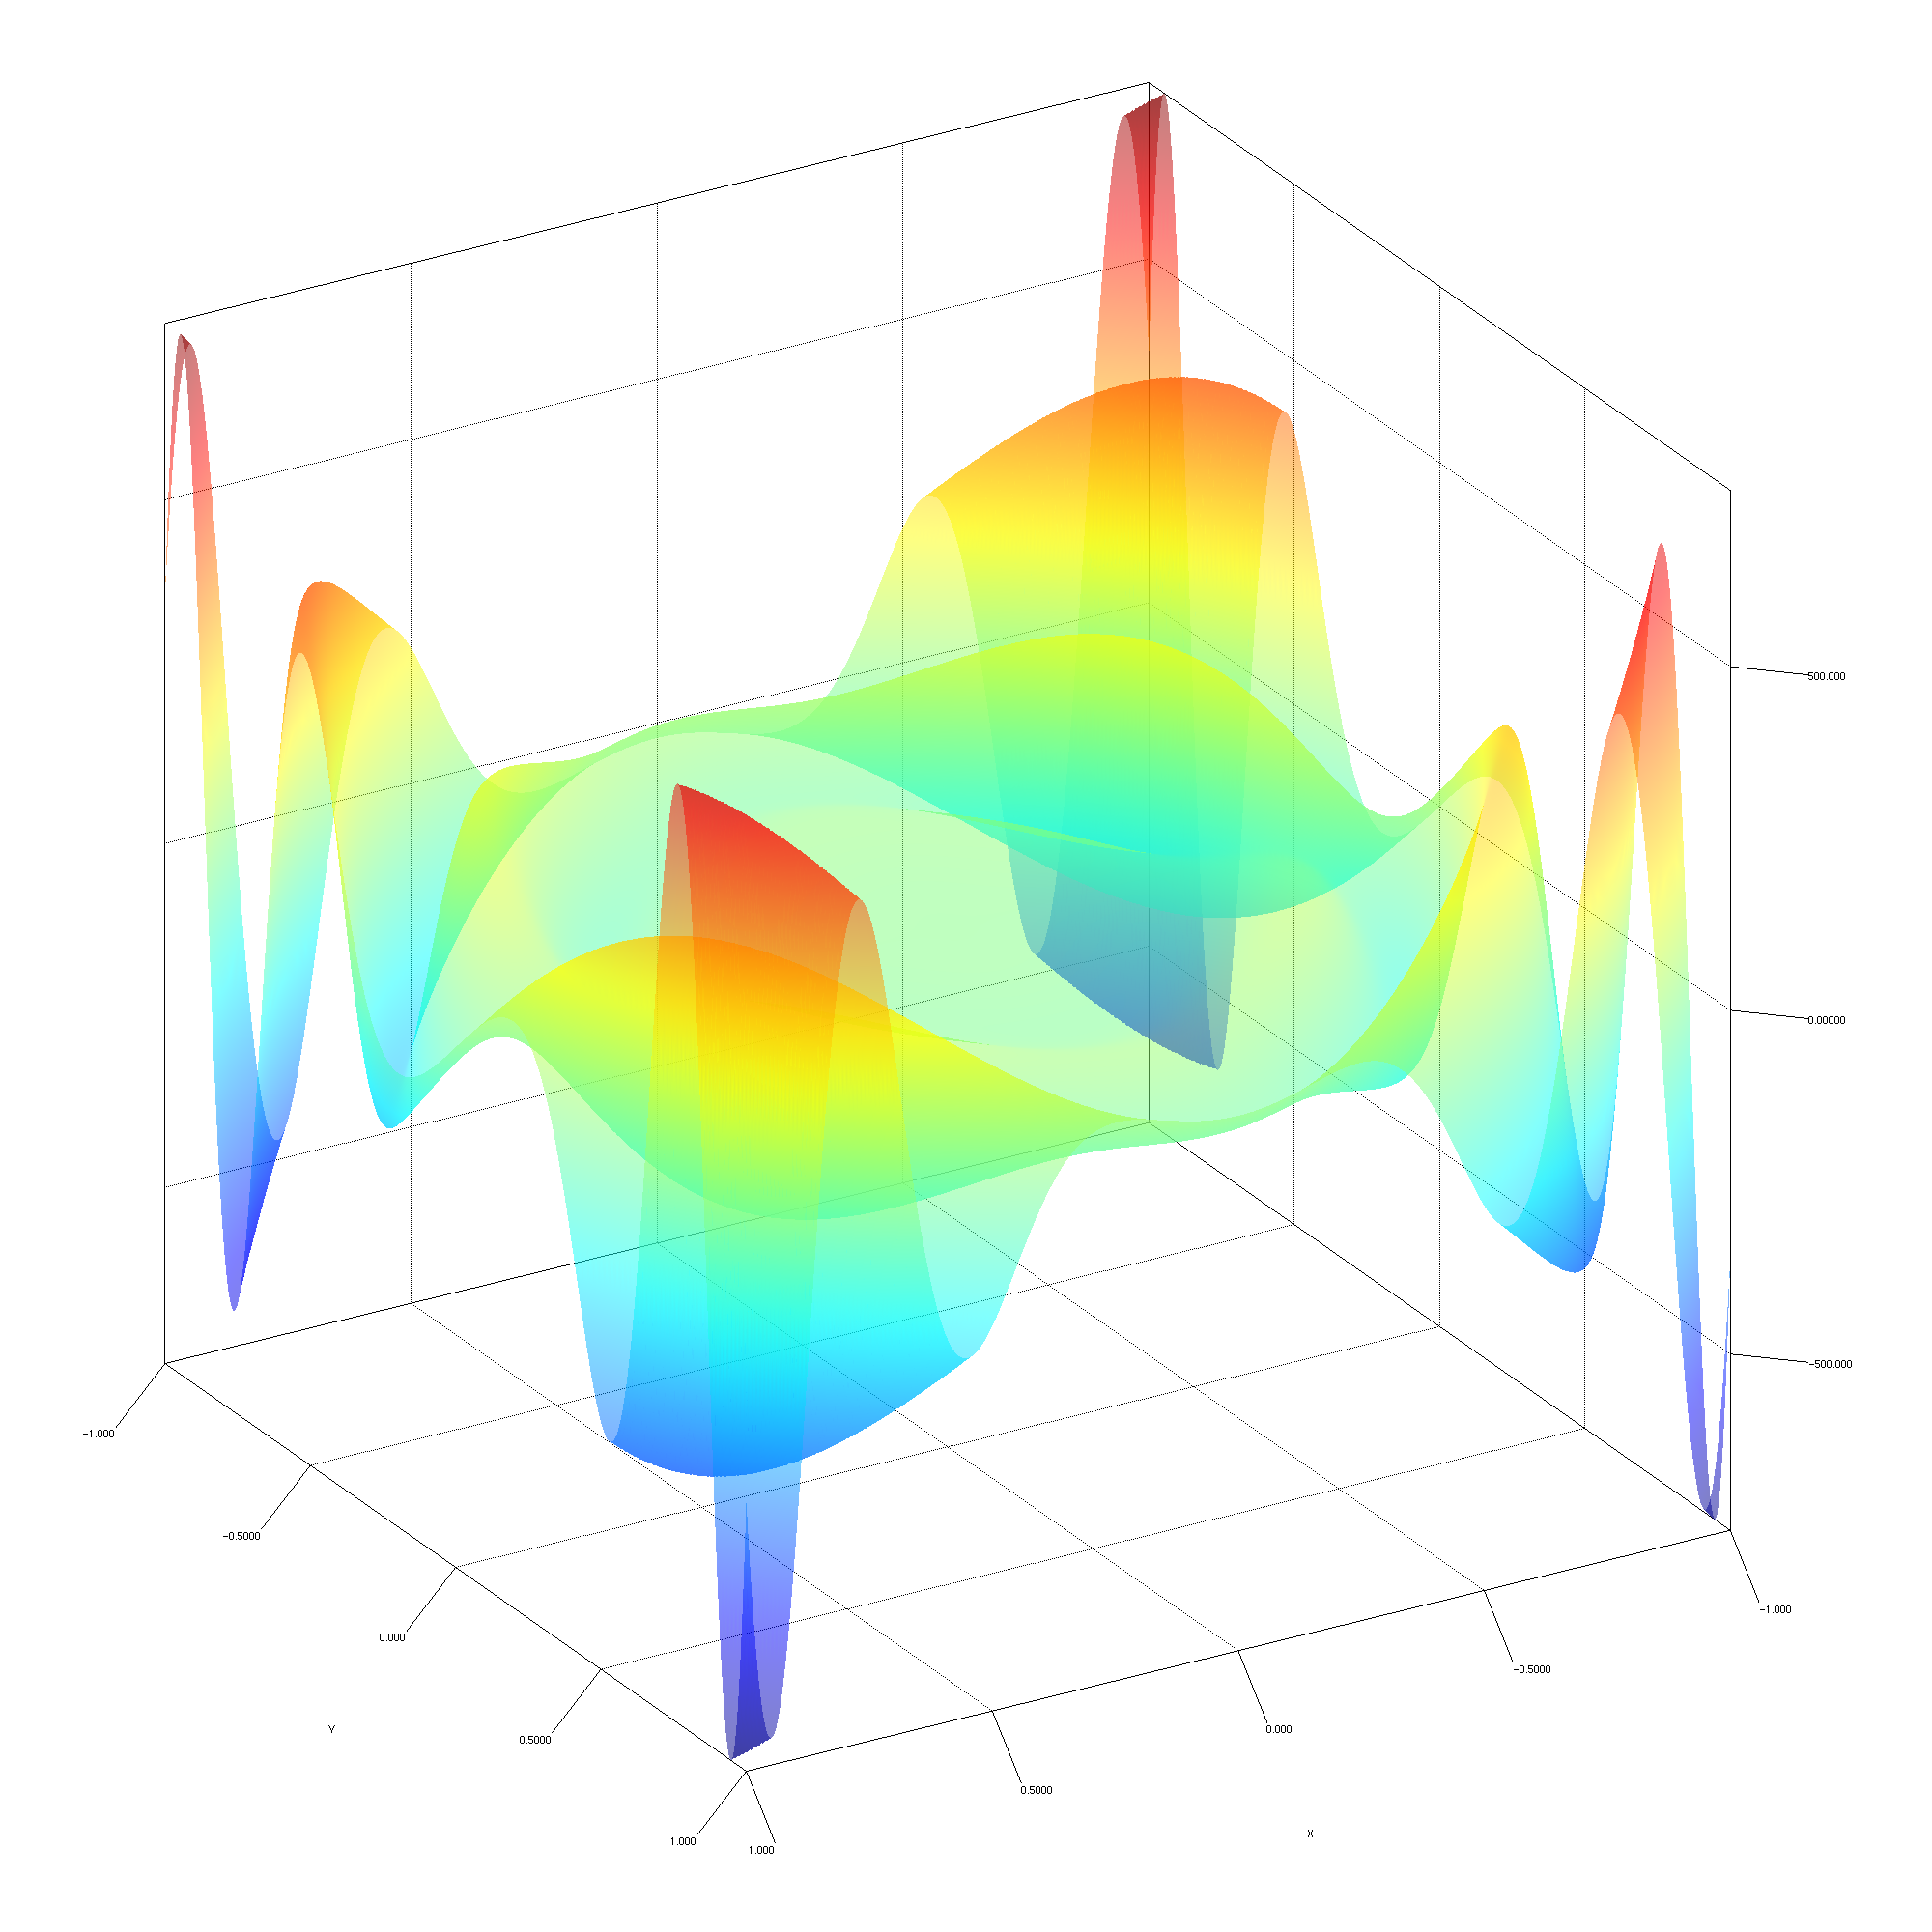
\includegraphics[scale=0.43]{plot_result.png}
\end{figure}
%
Above, we define a function with two variables and take a series of partial derivatives with respect to each variable. Expressions are lazily evaluated inside a numerical context, which may be imported on a per-file basis or lexically scoped for finer-grained control over the runtime behavior. The function is numerically evaluated on the interval $(-1, 1)$ in each dimension and rendered in 3-space. % We can also plot higher dimensional manifolds (e.g.\ the loss surface of a neural network), projected into four dimensions, and rendered in three, where one axis is represented by time.
%
\begin{figure}
\begin{unbreakablelisting}
val z = sin(10 * (x * x + pow(y, 2))) / 10 // Does not perform calculation
\end{unbreakablelisting}
\centering
\begin{tikzpicture}[grow=left]
    \tikzset{level distance=60pt}
    \Tree [.$\div$ [.\texttt{sin} [.$\times$ \texttt{10} [.$+$ [.$\times$ \texttt{\textbf{x}} \texttt{\textbf{x}} ] [.\texttt{pow} \texttt{\textbf{y}} \texttt{2} ] ] ] ] \texttt{10} ]
\end{tikzpicture}
\caption{Implicit DAG constructed by the original expression, \texttt{z}, seen above.}
    \label{lst:edsl}
\end{figure}

An expression is simply a DSL for constructing \texttt{Function}s. No numerical calculations, save for constant folding and algebraic simplification, are performed at this stage. Functions are only evaluated once invoked with numerical values, e.g. \texttt{z(0, 0)}.

\section{Type systems}\label{sec:type-systems}

Early work in type safe dimension analysis can be found in \citet{kennedy1994dimension, kennedy1996programming} showing how static types in array programming can be used to encode dimensionality and prevent common bugs due to dimension mismatch. Kennedy is particularly interested in units of measurement, and was followed by \citet{jay1996shape}, \citet{rittri1995dimension}, and \citet{zenger1997indexed}. Later, \citet{kiselyov2005number, kiselyov2010fun} and \citet{griffioen2015type}, show how to encode numbers to infer array sizes in more complex ways. More recently, with the resurgence of interest in tensor algebra and array programming, \citet{chen2017typesafe} and \citet{rink2018modeling} explore how shape safe tensor operations can be encoded in a sufficiently expressive type system.

The problem we would like to solve can be summarized as follows. Given two variables \inline{x} and \inline{y}, and operator $\diamond$, how do we determine whether the expression \inline{z = x} $\diamond$ \inline{y} is valid, and if so, what is the result type of \inline{z}? For matrix multiplication, when $\texttt{x} \in \mathbb{R}^{m \times n}$ and $\texttt{y} \in \mathbb{R}^{n \times p}$, the expression is well-typed and we can infer $\texttt{z} \in \mathbb{R}^{m \times p}$. More generally, we would like to infer the type of \inline{z} for some operator $\otimes: (\mathbb{R}^\mathbf{a}, \mathbb{R}^\mathbf{b}) \rightarrow \mathbb{R}^\mathbf{c}$ where $\mathbf{a} \in \mathbb{Z}^q, \mathbf{b} \in \mathbb{Z}^r, \mathbf{c} \in \mathbb{Z}^s$ and $q, r, s \in \mathbb{Z}^\geq$. For most linear algebra operations such as matrix multiplication, $\mathcal{T}(a, b) \stackrel{?}{=} c$ is computable in $\mathcal{O}(1)$ -- we can simply check the inner dimensions for equivalence and use the outer dimensions for inference.

Shape checking matrix operations is not always decidable, however. For arbitrary type functions $\mathcal{T}(\mathbf{a}, \mathbf{b})$, checking $\mathcal{T}(\mathbf{a}, \mathbf{b}) \stackrel{?}{=} \mathbf{c}$ requires a Turing machine, at which point it would be easier to compute at runtime rather than at the type level. If $\mathcal{T}$ is allowed to use the multiplication operator, as in the case of convolutional arithmetic~\citep{dumoulin2016guide}, shape inference becomes equivalent to Peano arithmetic, which is known to be undecidable~\citep{godel1931formal}. However shape checking convolutional arithmetic may be decidable.

First class dependent types are useful for ensuring arbitrary shape safety (e.g.\ when concatenating and reshaping matrices~\citep{xi1998eliminating}), but are unnecessary for simple equality checking, such as when multiplying two matrices.\footnote{Less expressive type systems are still capable of performing arbitrary computation in the type checker. As specified, Java's type system is known to be Turing Complete~\citep{Grigore:2017:JGT:3009837.3009871} It may be possible to emulate a limited form of dependent types in Java by exploiting this property, although this may not be computationally tractable due to the practical limitations noted by Grigore.} When the shape of a tensor is known at compile time, it is possible to shape check ordinary matrix arithmetic in a decidable type system with support for subtyping and parametric polymorphism. In practice, we can implement a shape-safe tensor algebra in any language with parametric types, such as Java, Kotlin, C++, Rust or Typescript, by enumerating a finite set of type-level integer literals, as shown in \autoref{sec:shape-safety}.

{\tiny
\begin{table}
    \begin{tabular}{|c|c|c|c|l|}
        \hline
        \multicolumn{1}{|c|}{Math$\dagger$}                    &  Infix                                                                         &  Prefix                                                                                 & Postfix                                                                                    & Type                                                                                                                                                                                    \\ \hline
                 $A(B)$                                        & \texttt{a(b)}                                                                  &                                                                                         &                                                                                            & $ (\texttt{a}:  \mathbb{R}^{\tau}\rightarrow\mathbb{R}^{\pi}, \texttt{b}: \mathbb{R}^{\lambda} \rightarrow \mathbb{R}^{\tau}) \rightarrow (\mathbb{R}^{\lambda}\rightarrow \mathbb{R}^{\pi}) $ \\ \hline
                 $A + B$                                       & \begin{tabular}{@{}c@{}}\texttt{a + b}\\\texttt{a.plus(b)}\end{tabular}        &  \texttt{plus(a, b)}                                                                    &                                                                                            & $ (\texttt{a}:  \mathbb{R}^{\tau}\rightarrow\mathbb{R}^{\pi}, \texttt{b}: \mathbb{R}^{\lambda} \rightarrow \mathbb{R}^{\pi}) \rightarrow (\mathbb{R}^{?}\rightarrow \mathbb{R}^{\pi}) $ \\ \hline
                 $A - B$                                       & \begin{tabular}{@{}c@{}}\texttt{a - b}\\\texttt{a.minus(b)}\end{tabular}       &  \texttt{minus(a, b)}                                                                   &                                                                                            & $ (\texttt{a}:  \mathbb{R}^{\tau}\rightarrow\mathbb{R}^{\pi}, \texttt{b}: \mathbb{R}^{\lambda} \rightarrow \mathbb{R}^{\pi}) \rightarrow (\mathbb{R}^{?}\rightarrow\mathbb{R}^{\pi})  $ \\ \hline
                 $A   B$                                       & \begin{tabular}{@{}c@{}}\texttt{a * b}\\\texttt{a.times(b)}\end{tabular}       &  \texttt{times(a, b)}                                                                   &                                                                                            & $ (\texttt{a}: \mathbb{R}^{\tau}\rightarrow\mathbb{R}^{m \times n}, \texttt{b}: \mathbb{R}^{\lambda}\rightarrow\mathbb{R}^{n \times p})    \rightarrow (\mathbb{R}^{?}\rightarrow\mathbb{R}^{m \times p})  $ \\ \hline
\begin{tabular}{@{}c@{}}$\frac{A}{B}$\\$AB^{-1}$\end{tabular}  & \begin{tabular}{@{}c@{}}\texttt{a / b}\\\texttt{a.div(b)}\end{tabular}         &  \texttt{div(a, b)}                                                                     &                                                                                            & $ (\texttt{a}: \mathbb{R}^{\tau}\rightarrow\mathbb{R}^{m \times n}, \texttt{b}: \mathbb{R}^{\lambda}\rightarrow\mathbb{R}^{p \times n}) \rightarrow (\mathbb{R}^{?}\rightarrow\mathbb{R}^{m \times p})     $ \\ \hline
\begin{tabular}{@{}c@{}}$-A$\\$+A$\end{tabular}                &                                                                                &  \begin{tabular}{@{}c@{}}\texttt{-a}\\\texttt{+a}\end{tabular}                          & \begin{tabular}{@{}c@{}}\texttt{a.unaryMinus()}\\\texttt{a.unaryPlus()}\end{tabular}       & $                   (\texttt{a}: \mathbb{R}^{\tau}\rightarrow\mathbb{R}^{\pi}) \rightarrow (\mathbb{R}^{\tau}\rightarrow\mathbb{R}^{\pi})                                             $ \\ \hline
\begin{tabular}{@{}c@{}}A+1 \\ A-1\end{tabular}                & \begin{tabular}{@{}c@{}}\texttt{a + 1}\\\texttt{a - 1}\end{tabular}            &  \begin{tabular}{@{}c@{}}\texttt{++a}\\\texttt{--a}\end{tabular}                        & \begin{tabular}{@{}c@{}}\texttt{a++, a.inc()}\\\texttt{a--, a.dec()}\end{tabular}          & $                 (\texttt{a}: \mathbb{R}^{\tau}\rightarrow\mathbb{R}^{m \times m}) \rightarrow (\mathbb{R}^{\tau}\rightarrow\mathbb{R}^{m \times m})                                               $ \\ \hline
\begin{tabular}{@{}c@{}}sin(a)\\cos(a)\\tan(a)\end{tabular}    &                                                                                &  \begin{tabular}{@{}c@{}}\texttt{sin(a)}\\\texttt{cos(a)}\\\texttt{tan(a)}\end{tabular} & \begin{tabular}{@{}c@{}}\texttt{a.sin()}\\\texttt{a.cos()}\\\texttt{a.tan()}\end{tabular}  & $                                            (\texttt{a}: \mathbb{R}\rightarrow\mathbb{R}) \rightarrow (\mathbb{R}\rightarrow\mathbb{R})                                              $ \\ \hline
                $\ln(A)$                                       &                                                                                &  \begin{tabular}{@{}c@{}}\texttt{ln(a)}\\\texttt{log(a)}\end{tabular}                   & \begin{tabular}{@{}c@{}}\texttt{a.ln()}\\\texttt{a.log()}\end{tabular}                     & $                  (\texttt{a}: \mathbb{R}^{\tau}\rightarrow\mathbb{R}^{m \times m}) \rightarrow (\mathbb{R}^{\tau}\rightarrow\mathbb{R}^{m \times m})                                              $ \\ \hline
               $\log_b A$                                      & \texttt{a.log(b)}                                                              &  \texttt{log(a, b)}                                                                     &                                                                                            & $       (\texttt{a}: \mathbb{R}^{\tau}\rightarrow\mathbb{R}^{m \times m}, \texttt{b}: \mathbb{R}^{\lambda}\rightarrow\mathbb{R}^{m \times m}) \rightarrow (\mathbb{R}^{?}\rightarrow\mathbb{R})     $ \\ \hline
                $A^{b}$                                        & \texttt{a.pow(b)}                                                              &  \texttt{pow(a, b)}                                                                      &                                                                                            & $       (\texttt{a}: \mathbb{R}^{\tau}\rightarrow\mathbb{R}^{m \times m}, \texttt{b}: \mathbb{R}^{\lambda}\rightarrow\mathbb{R}) \rightarrow (\mathbb{R}^{?}\rightarrow\mathbb{R}^{m \times m})     $ \\ \hline
\begin{tabular}{@{}c@{}}$\sqrt{a}$\\$\sqrt[3]{a}$\end{tabular} & \begin{tabular}{@{}c@{}}\texttt{a.pow(1.0/2)}\\\texttt{a.root(3)}\end{tabular} &  \begin{tabular}{@{}c@{}}\texttt{a.pow(1.0/2)}\\\texttt{a.root(3)}\end{tabular}         & \begin{tabular}{@{}c@{}}\texttt{a.sqrt()}\\\texttt{a.cbrt()}\end{tabular}                  & $                        (\texttt{a}: \mathbb{R}^{\tau}\rightarrow\mathbb{R}^{m \times m}) \rightarrow (\mathbb{R}\rightarrow\mathbb{R}^{m \times m})                                               $ \\ \hline
\begin{tabular}{@{}c@{}}$\frac{da}{db}$\\$a'(b)$\end{tabular}  & \texttt{a.diff(b)}                                                             &  \texttt{grad(a)[b]}                                                                    & \texttt{d(a) / d(b)}                                                                       & $                    (\texttt{a}: C(\mathbb{R}^{m})^{*}, \texttt{b}: \mathbb{R}\rightarrow\mathbb{R}) \rightarrow (\mathbb{R}^{m}\rightarrow\mathbb{R})                               $ \\ \hline
               $\nabla a$                                      &                                                                                &  \texttt{grad(a)}                                                                       & \texttt{a.grad()}                                                                          & $                   (\texttt{a}: C(\mathbb{R}^{m})) \rightarrow (\mathbb{R}^{m}\rightarrow\mathbb{R}^{m})                                                                         $ \\ \hline
    \end{tabular}
\caption{\label{tab:shape_system}Kotlin$\nabla$'s shape system specifies the output shape for matrix arithmetic.}
\end{table}
}
%$\dagger$ \texttt{a} and \texttt{b} are higher order functions. These may be constants (e.g. 0, 1.0), variables (e.g. \texttt{Var("x")}) or expressions (e.g. \texttt{x + 1}, \texttt{2 * x + y}).

\section{Shape safety}\label{sec:shape-safety}

\noindent There are three broad strategies for handling shape errors in array programming: \\
%
\begin{enumerate}
    \item Hide the error somehow by implicitly reshaping or broadcasting arrays.
    \item Announce the error at runtime with a relevant message, e.g.~\texttt{InvalidArgument}.
    \item Do not allow programs which can result in a shape error to compile. \\
\end{enumerate}
%
In Kotlin$\nabla$, we adopt the third strategy. Consider the following example:
%
\begin{kotlinlisting}
val a = Vec(1.0, 2.0) // Inferred type: Vec<Int, `2`>
val b = Vec(1.0, 2.0, 3.0) // Inferred type: Vec<Int, `3`>
val c = b + b
val d = a + b // Does not compile, shape mismatch
\end{kotlinlisting}
%
Attempting to sum two vectors whose shapes do not match will fail to compile.
%
\begin{kotlinlisting}
val a = Mat(`1`, `4`, 1.0, 2.0, 3.0, 4.0) // Inferred type: Mat<Double, `1`, `4`>
val b = Mat(`4`, `1`, 1.0, 2.0, 3.0, 4.0) // Inferred type: Mat<Double, `4`, `1`>
val c = a * b
val d = a * a // Does not compile, inner dimension mismatch
\end{kotlinlisting}
%
Similarly, multiplying two tensors whose inner dimensions do not match will not compile.
%
\begin{kotlinlisting}
val a = Mat(`2`, `4`,
            1.0, 2.0, 3.0, 4.0,
            5.0, 6.0, 7.0, 8.0)
val b = Mat(`4`, `2`,
            1.0, 2.0,
            3.0, 4.0,
            5.0, 6.0,
            7.0, 8.0)
val c: Mat<Double, `2`, `2`> = a * b // Types are optional, but encouraged
val d = Mat(`2`, `1`, 1.0, 2.0)
val e = c * d
val f = Mat(`3`, `1`, 1.0, 2.0, 3.0)
val g = e * f // Does not compile, inner dimension mismatch
\end{kotlinlisting}
%
It is required to specify the input types in a method signature. Explicit return types are optional but encouraged for readability. If omitted, the type system can usually infer them:
%
\begin{kotlinlisting}
fun someMatFun(m: Mat<Double, `3`, `1`>): Mat<Double, `3`, `3`> = ...
fun someMatFun(m: Mat<Double, `2`, `2`>) = ...
\end{kotlinlisting}
%
Shape safety is currently supported up to rank-2 tensors, i.e.\ matrices. To check shapes in our type system, we enumerate a list of integer type literals as a chain of subtypes, so that $C <: C - 1 <: C - 2 <: \dots <: 1 <: 0$, where $C$ is the largest fixed-length dimension we wish to represent. Using this encoding, we are guaranteed linear growth in space and time for subtype checking. $C$ can be specified by the user, who will need to regenerate the code.
%
\begin{kotlinlisting}[caption={Shape safe tensor addition for rank-1 tensors, $\forall C\leq2.$}]
interface Nat<T: `0`> { val i: Int }
// Integer literals have reified Int values should we need to compare them at runtime
sealed class `0`(open val i: Int = 0) { companion object: `0`(), Nat<`0`> }
sealed class `1`(override val i: Int = 1): `0`(i) { companion object: `1`(), Nat<`1`> }
sealed class `2`(override val i: Int = 2): `1`(i) { companion object: `2`(), Nat<`2`> }
sealed class `3`(override val i: Int = 3): `2`(i) { companion object: `3`(), Nat<`3`> }
//...Code for integer literals should be generated
sealed class `99`(override val i: Int = 99): `98`(i) { companion object: `99`(), Nat<`99`> }
\end{kotlinlisting}
%
Kotlin$\nabla$ supports shape-safe tensor operations by encoding tensor rank as a parameter of the operand type. Since integer literals are a chain of subtypes, we need only define tensor operations once using the highest literal, and can rely on Liskov substitution~\citep{liskov1987} to preserve shape safety for all subtypes. Consider the rank-1 tensor (i.e.\ vector) case:
%
\begin{kotlinlisting}
// <C: `1`> will accept 1 <= C <= 99 via Liskov substitution
infix operator fun <C: `1`, V: Vec<Float, C>> V.plus(v: V): Vec<Float, C> =
    Vec(length, contents.zip(v.contents).map { it.first + it.second })
\end{kotlinlisting}
%
The operator `\texttt{+}' can now be used like so. Incompatible operands will cause a type error:
%
\begin{kotlinlisting}
// Type-checked vector addition with shape inference
val Y = Vec(`2`, listOf(1, 2)) + Vec(`2`, listOf(3, 4)) // Y: Vec<Float, `2`>
val X = Vec(`2`, listOf(1, 2)) + Vec(`3`, listOf(3, 4, 5)) // Undefined!
\end{kotlinlisting}
%
This technique can be easily extended to additional infix operators. We can also define a shape-safe vector initializer by overloading the invoke operator on a companion object:
%
\begin{kotlinlisting}
open class Vec<E, Len: `1`> constructor(val len: Nat<Len>, val contents: List<E>) {
  companion object {
    operator fun <T> invoke(t: T): Vec<T, `1`> = Vec(`1`, listOf(t))
    operator fun <T> invoke(t0: T, t1: T): Vec<T, `2`> = Vec(`2`, listOf(t0, t1))
    operator fun <T> invoke(t0: T, t1: T, t2: T): Vec<T, `3`> = Vec(`3`, listOf(t0, t1, t2))
  }
}
\end{kotlinlisting}
%
Dynamic length construction is possible, although it may fail at runtime. For example:
%
\begin{kotlinlisting}
val one = Vec(`3`, 1, 2, 3) + Vec(`3`, 1, 2, 3)   // Always runs safely
val add = Vec(`3`, 1, 2, 3) + Vec(`3`, listOf(t)) // May fail at runtime
val vec = Vec(`2`, 1, 2, 3)                       // Does not compile
val sum = Vec(`2`, 1, 2) + add                    // Does not compile
\end{kotlinlisting}
%
A similar syntax is used for matrices and tensors. For example, Kotlin$\nabla$ can infer the shape of matrix multiplication, and will not compile if their inner dimensions disagree:
%
\begin{kotlinlisting}
val l = Mat(`4`, `4`, // Inferred type: Mat<Int, `4`, `4`>
             1, 2, 3, 4,
             5, 6, 7, 8,
             9, 0, 0, 0,
             9, 0, 0, 0)
val m = Mat(`4`, `3`, // Inferred type: Mat<Int, `4`, `3`>
             1, 1, 1,
             2, 2, 2,
             3, 3, 3,
             4, 4, 4)
val lm = l * m // Inferred type: Mat<Int, `4`, `3`>
val mm = m * m // Does not compile
\end{kotlinlisting}
%
This technique originates in Haskell, which supports more powerful forms of type-level computation, \textit{type arithmetic}~\citep{kiselyov2005number}. Type arithmetic makes it easy to express convolutional arithmetic~\citep{dumoulin2016guide} and other arithmetical operations on shape variables, which is currently not possible in Kotlin$\nabla$, or highly impractical as it would require enumerating every possible combination of type literals in type arithmetic.

\section{Testing}\label{sec:testing}

Kotlin$\nabla$ claims to eliminate certain runtime errors, but how do we know the proposed implementation is not incorrect? One method for checking is called property-based testing (PBT)~\citep{fink1997property} (c.f.~\autoref{subsec:property-based-testing}), which is borrowed from the Haskell community and closely related to the notion of metamorphic testing~\citep{chen1998metamorphic} (c.f.~\autoref{subsec:metamorphic-testing}). Notable implementations include QuickCheck~\citep{claessen2011quickcheck}, Hypothesis~\citep{Hypothesis} and KotlinTest~\citep{kotlintest}, on which our test suite is based. PBT uses algebraic properties to verify the result of an operation by constructing semantically equivalent but syntactically distinct expressions, which should produce the same answer. Kotlin$\nabla$ uses two such equivalences to validate its AD implementation: \\
%
\begin{enumerate}
    \item \textbf{Analytical differentiation}: manually differentiate selected functions and compare the numerical result of evaluating random chosen inputs from their domain with the numerical result obtained by evaluating AD on the same inputs.
    \item \textbf{Finite difference approximation}: sample the space of symbolic differentiable functions, comparing the numerical results suggested by the finite difference method and the equivalent AD result, up to a fixed-precision approximation. \\
\end{enumerate}
%
For example, the following test checks whether the analytical derivative and the automatic derivative, when evaluated at random points, are equal to within numerical precision:
%
\begin{kotlinlisting}
val x = Var("x")
val y = Var("y")
val z = y * (sin(x * y) - x)            // Function under test
val dz_dx = d(z) / d(x)                 // Automatic derivative
val manualDx = y * (cos(x * y) * y - 1) // Manual derivative

"dz/dx should be y * (cos(x * y) * y - 1)" {
    NumericalGenerator.assertAll { x0, y0 ->
        // Evaluate the results at a given seed
        val autoEval = dz_dx(x to x0, y to y0)
        val manualEval = manualDx(x to x0, y to y0)
        autoEval shouldBeApproximately manualEval // Fails iff eps < |adEval - manualEval|
    }
}
\end{kotlinlisting}
%
PBT will search the input space for two numerical values \inline{x0} and \inline{y0}, which violate the specification, then ``shrink'' them to discover pass-fail boundary values. We can construct a similar test with the finite difference method, which uses the equation $f'(x) \approx \frac{f(a+h)-f(a)}{h}$:
%
\begin{kotlinlisting}
val dx = 1E-8
val x = Var("x")
val f = sin(x)
val df_dx = d(f) / d(x)
val fd_dx = (sin(x + dx) - sin(x)) / dx

"d(sin x)/dx should be equal to (sin(x + dx) - sin(x)) / dx" {
    NumericalGenerator.assertAll { x0 ->
        val autoEval = df_dx(x0)
        val fdEval = fd_dx(x0)
        autoEval shouldBeApproximately fdEval // Fails iff eps < |adEval - fdEval|
    }
}
\end{kotlinlisting}
%
There are many other ways to independently verify the numerical gradient, such as dual numbers or the complex step derivative. Another method would be to compare the numerical output against a well-known implementation, such as TensorFlow. In future work, we intend to conduct a more thorough comparison of numerical accuracy and performance.

\section{Operator overloading}\label{sec:operator-overloading}

\noindent Operator overloading enables a concise notation for arithmetic on abstract types, where the types encode algebraic structures, e.g. \inline{Group}, \inline{Ring}, and \inline{Field}. These abstractions are extensible to other mathematical structures, such as complex numbers and quaternions.

For example, we have an interface \inline{Group} which overloads the operators $+$ and $\times$:
%
\begin{kotlinlisting}
interface Group<T: Group<T>> {
    operator fun plus(addend: T): T
    operator fun times(multiplicand: T): T
}
\end{kotlinlisting}
%
Here, we specify a recursive type bound using a method known as F-bounded polymorphism~\citep{canning1989f} to ensure that operations return the concerete value of the type variable \inline{T}, rather than something more generic like \inline{Group} (effectively, \inline{T} is a \inline{self} type). Imagine a class \inline{Fun} which has implemented \inline{Group}. It can be used as follows:
%
\begin{kotlinlisting}
fun <T: Group<T>> cubed(t: T): T = t * t * t
fun <X: Fun<X>> twiceExprCubed(e: X): X = cubed(e) + cubed(e)
\end{kotlinlisting}
%
Like Python, Kotlin supports overloading a limited set of operators, which are evaluated using a fixed precedence. In the current version of Kotlin$\nabla$, operators do not perform any computation, they simply construct a directed acyclic graph representing the symbolic expression. Expressions are only evaluated when invoked as a function.

\section{First class functions}\label{sec:first-class-functions}

With support for higher-order functions and lambdas, Kotlin treats functions as first class citizens. This allows us to represent mathematical functions and programming functions with the same underlying abstractions (i.e.\ typed FP). Following a number of recent papers in functional AD~\citep{pearlmutter2008reverse,wang2018backpropagation}, in Kotlin$\nabla$, all expressions are treated as functions. For example:

\begin{kotlinlisting}
fun <T: Group<T>> makePoly(x: Var<T>, y: Var<T>) = x * y + y * y + x * x
val x: Var<DoubleReal> = Var()
val y: Var<DoubleReal> = Var()
val f = makePoly(x, y)
val z = f(1.0, 2.0) // Returns a value
println(z) // Prints: 7
\end{kotlinlisting}

Currently, it is possible to represent functions where all inputs and outputs share a single data type. It is possible to extend support for building functions with varying input/output types and enforce constraints on both, using covariant and contravariant type bounds. We leave this for further work.

\section{Numeric Tower}\label{sec:numeric-tower}

Kotlin$\nabla$ uses a numeric tower~\citep{st2012typing}. First pioneered in the functional programming language, Scheme~\citep{sperber2009revised}, this strategy is also suited to object oriented programming~\citep{niculescu2003design, niculescu2011using} and widely used in other JVM libraries such as KMath~\citep{nozik2019acat} and Apache Commons Math~\citep{developers2012apache}.

\begin{kotlinlisting}[caption={Most mathematical operations are composed of a small set of simple operators.}]
interface Group<X: Group<X>> {
    operator fun unaryMinus(): X
    operator fun plus(addend: X): X
    operator fun minus(subtrahend: X): X = this + -subtrahend
    operator fun times(multiplicand: X): X
}

interface Field<X: Field<X>>: Group<X> {
    val e: X
    val one: X
    val zero: X
    operator fun div(dividend: X): X = this * dividend.pow(-one)
    infix fun pow(exp: X): X
    fun ln(): X
}
\end{kotlinlisting}

The numeric tower also allows us to define common behavior such as subtraction and division on abstract algebraic structures, which are easily extended to concrete number systems. For example, to later define a field over the complex numbers or other algebras,~\footnote{ex. In order to calculate derivatives in a quaternion neural network.\citep{isokawa2003quaternion}} one must simply extend the numeric tower and override the default implementation. Most mathematical operations can be defined by composing a small set of primitive operations, which can later be differentiated in a generic fashion, rather than on an ad hoc basis.

\section{Algebraic data types}\label{sec:adts}

\noindent Algebraic data types (ADTs) in the form of sealed classes (a.k.a.\ sum types) facilitate a limited form of pattern matching over a closed set of subclasses. When matching against subclasses of a sealed class, the compiler forces the author to provide an exhaustive control flow over all concrete subtypes of an abstract class. Consider the following classes:
%
\begin{kotlinlisting}
class Const<T: Fun<T>>(val number: Number) : Fun<T>()
class Sum<T: Fun<T>>(val left: Fun<T>, val right: Fun<T>) : Fun<T>()
class Prod<T:Fun<T>>(val left: Fun<T>, val right: Fun<T>) : Fun<T>()
class Var<T: Fun<T>>: Fun<T>() { override val variables: Set<Var<X>> = setOf(this) }
class Zero<T: Fun<T>>: Const<T>(0.0)
class One<T: Fun<T>>: Const<T>(1.0)
\end{kotlinlisting}
%
When branching on the type of a sealed class, consumers must explicitly handle every subclass, since incomplete control flow will not compile, rather than fail silently at runtime.
%
\begin{kotlinlisting}
sealed class Fun<X: Group<X>>(open val variables: Set<Var<X>> = emptySet()): Group<Fun<X>> {
    constructor(vararg fns: Fun<X>): this(fns.flatMap { it.variables }.toSet())

    // Since the subclasses of Fun are a closed set, no `else -> ...` is required.
    operator fun invoke(map: Map<Var<X>, X>): Fun<X> = when (this) {
        is Const -> this
        is Var -> map.getOrElse(this) { this }
        is Prod -> left(map) * right(map) // Smart casting implicitly casts after checking
        is Sum -> left(map) + right(map)
    }

    fun diff(): Fun<X> = when(this) {
       is Const -> Zero
       is Var -> One
       // Product rule: d(u*v)/dx = du/dx * v + u * dv/dx
       is Prod -> left.diff() * right + left * right.diff()
       is Sum -> left.diff() + right.diff()
    }

    operator fun plus(addend: Fun<T>) = Sum(this, addend)

    operator fun times(multiplicand: Fun<T>) = Prod(this, multiplicand)
}
\end{kotlinlisting}
%
Kotlin's smart-casting implicitly downcasts the abstract type \inline{Fun} as a subtype, e.g. \inline{Sum} after performing an \inline{is Sum} check. Otherwise, we would need to write \inline{(this as Sum).left} in order to access its member, \inline{left}. If the type cast was mistaken, a \inline{ClassCastException} would be thrown, which smart casting also prevents.

\section{Multiple Dispatch}\label{sec:multiple-dispatch}

In conjunction with ADTs, Kotlin$\nabla$ also uses multiple dispatch to instantiate the most specific result type of applying an operator based on the type of its operands. While multiple dispatch is not an explicit language feature, it can be emulated using inheritance.

Building on the previous example, suppose we would like to perform algebraic simplification. This can be useful for reducing expression swell and improving numerical stability. We can use multiple dispatch to branch on a the type of a subexpression at runtime. \textit{Smart casting} lets us access  members of a class after checking its type, as if it were casted:

\begin{kotlinlisting}
override fun times(multiplicand: Fun<X>): Fun<X> =
    when {
        this == zero -> this
        this == one -> multiplicand
        multiplicand == one -> this
        multiplicand == zero -> multiplicand
        this == multiplicand -> pow(two)
        // w/o smart cast: Const((this as Const).number * (multiplicand as Const).number)
        this is Const && multiplicand is Const -> Const(number * multiplicand.number)
        // Further simplification is possible using rules of replacement
        else -> Prod(this, multiplicand)
    }

val result = Const(2.0) * Sum(Var(2.0), Const(3.0))
//         = Sum(Prod(Const(2.0), Var(2.0)), Const(6.0))
\end{kotlinlisting}

Multiple dispatch allows us to put all related control flow on a single abstract class which is inherited by subclasses, simplifying readability, debugging and refactoring.

\section{Extension Functions}\label{sec:extension-functions}

Extension functions augment external classes with new fields and methods. By using context oriented programming~\citep{hirschfeld2008context}, we can expose custom extensions (e.g.\ through \inline{DoubleContext}) to consumers without requiring subclassing or inheritance.
%
\begin{kotlinlisting}[caption={We can provide numerical extensions, wrapped in a context.}]
data class Const<T: Fun<T>>(val number: Double) : Fun<T>()
data class Sum<T: Fun<T>>(val left: Fun<T>, val right: Fun<T>) : Fun<T>(left, right)
data class Prod<T: Fun<T>>(val left: Fun<T>, val right: Fun<T>) : Fun<T>(left, right)
object DoubleContext {
    operator fun Number.times(expr: Fun<Double>) = Const(toDouble()) * expr
}
\end{kotlinlisting}
%
Now, we can use the context to define another extension, \inline{Fun.multiplyByTwo}, which computes the product inside a \inline{DoubleContext}, using the operator overload defined above:
%
\begin{kotlinlisting}
fun Fun<Double>.multiplyByTwo() = with(DoubleContext) { 2 * this }
\end{kotlinlisting}
%
Extensions can also be defined in another file or context and imported on demand. This approach was borrowed from KMath~\citep{nozik2019acat}, another mathematical library for Kotlin.

\section{Automatic, Symbolic Differentiation}

It has long been claimed by the AD literature that automatic differentiation is not symbolic differentiation~\citep{baydin-survey}. Many, including the author of this thesis, has suspected this claim to be misleading. Recently, the claim has been questioned~\citep{wang2018demystifying} and refuted~\citep{laue2019equivalence}. While it may be true that certain implementations of automatic differentiation interleave numerical and symbolic differentiation during a program's execution, interleaving differentiation and numerical execution is certainly not a prerequisite for a differentiation library to be considered \textit{automatic}, particularly when popular AD implementations, such as Theano~\citep{theano}, have chosen the symbolic route. It is our view that symbolic differentiation is one type of automatic differentiation, in particular, one which affords more flexibility to perform global optimizations and rewriting procedures. These optimizations would otherwise be impossible if attempted at runtime, with only partial information about the graph.

\section{Coroutines}\label{sec:coroutines}

Coroutines are a generalization of subroutines for non-preemptive multitasking, typically implemented using continuations. Continuations are a mechanism that allow functions to access and modify subsequent computation. In continuation passing style (CPS), every function, in addition to its usual arguments, takes a second function representing the subsequent computation to be performed. Rather than returning to its caller, the function invokes its continuation immediately prior to completion, and the process is restarted. If the continuation is empty, the program halts.

One form of continuation, known as shift-reset a.k.a.\ delimited continuations, are sufficient for implementing reverse mode AD with operator overloading alone (without any additional data structures) as described by \textit{Shift/Reset the Penultimate Backpropagator}~\citep{wang2018demystifying} and later in \textit{Backpropagation with Continuation Callbacks}~\citep{wang2018backpropagation}. Delimited continuations can be implemented with Kotlin's Coroutines support.

\section{Comparison}\label{sec:comparison}

Inspired by Stalin$\nabla$, Autograd, DiffSharp, Myia, Nexus, Lantern, Tangent et al., Kotlin$\nabla$ attempts to port recent developments in automatic differentiation (AD) to the Kotlin language. It introduces a number of experimental ideas, including compile-time shape-safety, algebraic simplification and numerical stability checking through property-based testing. Unlike most existing automatic differentiation libraries, Kotlin$\nabla$ is a purely symbolic, graph-based solution that does not require any compiler augmentation or runtime reflection. As we have seen, it achieves this primarily through operator overloading, polymorphism, and pattern matching. The practical advantage of this approach is that it can be implemented as a simple library or \textit{embedded domain-specific language}, thereby employing the host language's type system. Our approach is particularly well-suited to functional programming, and makes use of a number of functional programming concepts, including lambda expressions, higher order functions, partial application, and algebraic data types. \\

\begin{table}
\begin{tabular}{lllllllll}
    Framework &
    Language &
    \rot{Symbolic Differentiation} &
    \rot{Automatic Differentiation} &
    \rot{Functional Programming} &
    \rot{Type Safe} &
    \rot{Shape Safe} &
    \rot{Differentiable Programming} &
    \rot{Multiplatform}
    \\ \hline
Kotlin$\nabla$     & Kotlin  & \cmark & \cmark & \cmark & \cmark & \cmark & \wmark & \wmark \\
DiffSharp          & F\#     & \xmark & \cmark & \cmark & \cmark & \xmark & \cmark & \xmark \\
TensorFlow.FSharp  & F\#     & \xmark & \cmark & \cmark & \cmark & \cmark & \cmark & \xmark \\
Myia               & Python  & \cmark & \cmark & \cmark & \cmark & \cmark & \cmark & \xmark \\
Deeplearning.scala & Scala   & \xmark & \cmark & \cmark & \cmark & \xmark & \cmark & \xmark \\
Nexus              & Scala   & \xmark & \cmark & \cmark & \cmark & \cmark & \cmark & \xmark \\
Lantern            & Scala   & \xmark & \cmark & \cmark & \cmark & \xmark & \cmark & \xmark \\
Grenade            & Haskell & \xmark & \cmark & \cmark & \cmark & \cmark & \xmark & \xmark \\
Eclipse DL4J       & Java    & \cmark & \cmark & \xmark & \cmark & \xmark & \xmark & \xmark \\
Halide             & C++     & \xmark & \cmark & \xmark & \cmark & \xmark & \cmark & \xmark \\
Stalin$\nabla$     & Scheme  & \xmark & \cmark & \cmark & \xmark & \xmark & \xmark & \xmark \\
\end{tabular}
\caption{Comparison of AD libraries. The \wmark symbol indicates work in progress.}
\end{table}

\section{Future work}\label{sec:future-work}

Allowing users to specify a matrix's structure in its type signature, (e.g.\ Singular, Symmetric, Orthogonal, Unitary, Hermitian, Toeplitz) would allows us to specialize derivation over such matrices (c.f. section 2.8 of~\citet{petersen2008matrix} for a detailed review of specific techniques for calculating derivatives of structured matrices).

Integration with a dedicated linear algebra backend such as ND4J~\citep{team2016nd4j}, Apache Commons Math~\citep{developers2012apache}, EJML~\citep{abeles2010efficient} or JBlas~\citep{braun2011jblas}. Look into~\cite{makwana2018numlin}.

Explore the meaning of derivatives in other calculi, and incremental compilation following~\citet{ehrhard2003differential, chen2012type, cai2014theory, kelly2016evolving}.

\medium{\chapter{Testing and validation}\label{ch:difftest}}

\setlength{\epigraphwidth}{0.80\textwidth}
\epigraph{``If we use, to achieve our purposes, a mechanical agency with whose operation we cannot efficiently interfere\ldots then we had better be quite sure the purpose put into the machine is the purpose which we really desire.''}{\begin{flushright}--Norbert \citet{wiener1960some}, \textit{Some moral and technical consequences of automation}~\end{flushright}}

Today's deep neural networks are surprisingly effective when compared with handcrafted algorithms, but have known weaknesses. Training neural networks which can robustly transfer to new domains where the training and test distributions are dissimilar continues to pose a significant challenge. Furthermore, such models are susceptible to failure when presented with carefully crafted inputs. However the same gradient-based optimization techniques used for training neural networks can also be exploited to probe their failure modes.

In software engineering, techniques for software testing have become increasingly more automated and general purpose. Developers love to write code, but loath writing tests. Yet tests are essential to validate an implementation's correctness. Tests prevent regressive behavior and are a form of specification in which the developer communicates the intended result of running a program. Techniques in coverage-guided fuzzing enable developers to write fewer tests with higher coverage. This is possible by automated testing.

In this chapter, we will explore the relationship between testing in machine learning and software engineering. We will see how the notion of adversarial testing shares a curious resemblance to fuzz testing in software engineering. In particular, we show how probabilistic sampling and constrained optimization can be seen as an extension of property-based testing (PBT) for adversarial training of differentiable programs, and propose a PBT algorithm which incorporates features of probabilistic programming and gradient-based optimization.

\subsection{Unit Testing}

In traditional unit testing, most tests are written in the following manner:

\begin{kotlinlisting}
fun unitTest() {
    val input = 1
    val expectedOutput = 2
    val actualOutput = program(input)
    assertEquals(actualOutput, expectedOutput)
}
\end{kotlinlisting}

The trouble is, someone needs to sit down and write a bunch of test cases.

\subsection{Fuzz Testing}

Fuzz testing is an automated software testing methodology which automatically generates test inputs in order to break a known function. For example, consider the following test:

\begin{kotlinlisting}
fun simpleFuzzTest() {
    val inputs = generateRandomInputs()
    for(i in inputs)
        assertEquals(program(i), oracle(i))
}
\end{kotlinlisting}

The trouble is, we need an oracle, an often unreasonable assumption. This is known as the test oracle problem. Furthermore, even if we had an oracle, if the space of inputs is large, it can take a long time to find an input where they disagree. Furthermore, since a single call to \inline{program(i)} can be be quite expensive in practice, this method can be inefficient.

\subsection{Property-based Testing}\label{subsec:property-based-testing}

Property-based testing (PBT) is a specific type of fuzz testing which addresses the test oracle problem by using properties. PBT has two phases, seaching and shrinking. It can be seen as follows:

\begin{kotlinlisting}
fun propertyBasedTest() {
    val inputs = generateRandomInputs()
    for(i in inputs)
        output = program(i)
        if (output !has property)
            shrink(i, program, property)
}
\end{kotlinlisting}

Roughly speaking, \inline{shrink} attempts to find the minimal breaking example. For example, if \inline{program} has type \inline{(Float) -> T}, a na\"ive shrinker might be implemented as follows:

\begin{kotlinlisting}
tailrec fun shrink(input: Float, program: (Float) -> T, property: (T) -> Boolean) =
    if(program(input) has property) return
    if(program(input - input / 2.0f) has property)
        assert("Minimal output lacking $property:" + program(input))
    else shrink(input - input / 2.0f, program, property)
\end{kotlinlisting}

The trouble is, finding the right properties to test can be highly sensitive, and requires a lot of effort and domain-specific expertise. What if there were a better way?

\subsection{Metamorphic testing}\label{subsec:metamorphic-testing}

Metamorphic testing is a fuzz testing methodology which addresses the test oracle problem, and specifically the challenge of designing low-cost, general-purpose properties. It has been successfully applied in testing driverless cars~\citep{zhou2019metamorphic, pei2017deepxplore, tian2018deeptest} and other stateful deep learning systems~\citep{du2018deepcruiser}.

More precisely, it can be expressed as follows: Given an oracle $\mathbf P: Q \rightarrow S$, a set of inputs $X = \{\mathbf{x}^{(0)}, \dots, \mathbf{x}^{(z)}\}$ and outputs $\{\mathbf{y}^{(0)} = \mathbf{P}(\mathbf{x}^{(0)}), \dots, \mathbf{y}^{(z)} = \mathbf{P}(\mathbf{x}^{(z)})\}$, a metamorphic relation (MR) is a relation $\mathcal R \subset Q^z \times S^z$ where $z \geq 2$. In the simplest case, an MR is a equivalence relation over input-output pairs, where e.g., $\langle \mathbf x, \mathbf y \rangle \mathcal R \langle \mathbf x', \mathbf y' \rangle \Leftrightarrow \mathbf P(\mathbf x) = \mathbf P(\mathbf x')$.

For example, suppose that our MR is $\mathbf P(\mathbf x) = \mathbf P(\mathbf x' = \mathbf x + \varphi) = \mathbf y, \forall \varphi \in [0, \varepsilon]$. Given a small set of pairs from an oracle $\langle \mathbf x, \mathbf y \rangle \in \mathbf P$, and a program $\mathbf{\hat P}$, the MR suggests a much larger set of inputs on which to test $\mathbf{\hat P}$, without requiring matched outputs from the oracle $\mathbf P$. If $\exists \mathbf x' \in \{\mathbf x: |\mathbf x - \mathbf x'| < \varepsilon\}$, this implies $\mathcal R$ does not hold on $\mathbf{\hat P}$ and either:

\begin{enumerate}
\item the MR is invalid $(\langle \mathbf x, \mathbf P(\mathbf x)\rangle, \langle \mathbf x', \mathbf P(\mathbf x')\rangle) \notin \mathcal R$, or
\item $\mathbf{\hat P} != \mathbf{P}$ the program under test is broken.
\end{enumerate}

Consider a more concrete example: suppose we have a function that should predict the correct steering angle for an image of a road. Assume we are given a single image and the ground truth steering angle. One metamorphic relation could be invariance under changes to lighting, small rotations, shifts or skews of the image. We should be able to apply any single transformation or permutation of composed transformations on the image, and the output ought to remain unchanged. If the output is drastically different in some way, we have detected an error.

TODO: code

\subsection{Adversarial Testing}

During backpropogation we perform gradient descent on a differentiable function with respect to its parameters for a specific set of inputs. In adversarial testing, we do gradient descent on a loss function with respect to the input(s) at a fixed parameter setting.

\section{Background}
%
\noindent Suppose we have a differentiable vector function $\mathbf{\hat P}: \mathbb{R}^n\rightarrow\mathbb{R}^m$:
%
\begin{equation} \tag{\autoref{eq:recursive_parametric_eq} revisited}
    \mathbf{\hat P}_k(\mathbf{x}; \mathbf{\Theta}) = \begin{cases} \mathbf{\hat p}_0(\mathbf\theta_0)(\mathbf{x}) &\text{if } k=0\\ \big(\mathbf{\hat p}_k(\mathbf\theta_k)\circ \mathbf{\hat P}_{k-1}(\mathbf{\Theta}_{[0, k-1]})\big(\mathbf{x}\big)&\text{if } k > 0 \end{cases} \\
\end{equation}
%
In deep learning, given pairs $\mathbf{X} = \{\mathbf{x}^{(0)}, \dots, \mathbf{x}^{(z)}\}, \mathbf{Y} = \{\mathbf{y}^{(0)} = \mathbf{P}(\mathbf{x}^{(0)}), \dots, \mathbf{y}^{(z)} = \mathbf{P}(\mathbf{x}^{(z)})\}$ we want to find $\mathbf{\Theta}^* = \argmin{\boldsymbol{\Theta}}\mathcal{L}\big(\mathbf{\hat P}_k(\mathbf{x}^{(i)}; \mathbf{\Theta}), \mathbf{y}^{(i)}\big)$ which is typically achieved by performing stochastic gradient descent on the loss with respect to the model parameters:
%
\begin{equation} \tag{\autoref{eq:stochastic_grad_descent} revisited}
    \mathbf\Theta \leftarrow \mathbf\Theta - \alpha\frac{1}{z}\nabla_{\mathbf\Theta} \sum_{i=0}^z\mathcal{L}\big(\mathbf{\hat P}_k(\mathbf{x}^{(i)}; \mathbf{\Theta}), \mathbf{y}^{(i)}\big)
\end{equation}
%
In the white box adversarial learning setting, we are given a fixed $\mathbf \Theta$\footnote{In contrast with backpropogation, where the parameters $\mathbf\Theta$ are updated.} and control the value of $\mathbf x$, so we can rewrite $\mathbf{\hat P}_k(\mathbf{x}^{(i)};\mathbf\Theta)$ instead as $\mathbf{\hat P}(\mathbf x)$. Our goal is to find the worst X:
%
\begin{equation}
\mathbf{x}^* = \argmax{\mathbf{x}}\mathcal{L}\big(\mathbf{\hat P}(\mathbf{x}), \mathbf{y}^{(i)}\big) \text{ subject to } CS = \{\mathbf{x} \in \mathbb{R}^n \text{ s.t. } ||\mathbf{x}^{(i)} - \mathbf{x}|| < \epsilon\}
\end{equation}
%
 To do so, initialize $\mathbf{x} \sim U[CS]$ and perform projected gradient descent on the loss w.r.t. $\mathbf x$:
%
\begin{equation}\label{eq:projected_gd}
    \mathbf x \leftarrow \mathbf{\Phi}_{CS}\Big(\mathbf x - \alpha\mathbf\nabla_{\mathbf x} \mathcal{L}\big(\mathbf{\hat P}(\mathbf{x}), \mathbf{y}^{(i)}\big)\Big) \text{, where }
	\mathbf{\Phi}_{CS}(\mathbf \phi') = \argmin{\mathbf \phi \in CS}\frac{1}{2}||\mathbf \phi - \mathbf \phi'||^2_2
\end{equation}
%
Henceforth we shall refer to $\mathcal{L}\big(\mathbf{\hat P}(\mathbf{x}), \mathbf{y}^{(i)}\big)$ as $\mathcal{L}(\mathbf x)$. Imagine a single test $\mathbf{T}: \mathbb{R}^n \times \mathbb{R} \rightarrow \mathbb{B}$:
%
\begin{equation} \label{eq:output_constraint_example}
    \mathbf T(\mathbf{\hat P}, \mathbf{x}) = \mathcal{L}(\mathbf{x}) < C
\end{equation}
%
Where $C \in \mathbb{R}$. How can we find a set of inputs that break the test under a fixed computational budget (i.e.\ constant number of program evaluations)? In other words:
%
\begin{equation}
    D_\mathbf T: \{ x \sim \mathbb{R}(0, 1) \mid \mathbf{\hat P}(\mathbf x) \implies \neg \mathbf T \}, maximize |D_\mathbf T|
\end{equation}
%
If if the tester has no knowledge about the programs implementation or its data distribution, $D_\mathbf\hat P$, it can do no better than random search~\citep{wolpert1997no}. However, if she has some information about the input distribution, she could re-parameterize the distribution to incorporate her knowledge. Assuming the program has previously been tested on common inputs, she might sample $x \sim \frac{1}{D_\mathbf\hat P}$ for inputs that are infrequent. If the tester knew how $\mathbf{\hat P}$ were implemented, she could use classical fuzzing techniques to prioritize the search procedure. But these methods are not specialized to continuous differentiable functions.

% Finally, we could train a neural network to predict inputs that were likely to cause a program to fail a given specification. As input, the network would take the function and test cases, and as its output, produce values that were likely to violate $T$.

Another strategy, independent of how candidate inputs are selected, is to use some form of gradient based optimization in the search procedure. If the tester does not have access to the function directly, she can still use zeroth order optimization techniques to approximate the gradient. Given access to the program, she can compute the gradient of the program using automatic differentiation. The gradient of $\mathbf{\hat P}$'s loss with respect to $\mathbf{x}$ is $\nabla_{\mathbf{x}} \mathcal{L}(\mathbf x)$.
%

% Furthermore, we hypothesize that if a sufficiently large fraction of the input space existed where $T$ were false, then as we sample from that space, the probability of detection would approach 1:
%
% \begin{equation}
%     (\forall i \in I^\dagger, p(i) \implies \neg T) \implies \lim_{|x|\to \infty}Prob(\hat{T}=False) = 1
% \end{equation}
%

Consider algorithm \autoref{alg:prob_fuzz} for finding test failures. First, let us select a candidate input $\mathbf{x}_j$ according to sampling strategy $\mathcal S$ (e.g.\ uniform random, or a neural network which takes $\mathbf{\hat P}$ and $\mathbf T$ as input). If $\mathbf{\hat P}(\mathbf{x}^i)$ violates $\mathbf T$, we can append $\mathbf x^i$ to $D_\mathbf T$ and repeat. Otherwise, we follow the gradient of $\mathcal{L}(\mathbf{\hat P}, \mathbf{x})$ with respect to $\mathbf{x}$ and repeat until test failure, gradient descent convergence, or a fixed number of steps $C$ are reached before resampling $\mathbf{x}$ from the initial sampling strategy $\mathcal S_n$ to ensure each gradient descent trajectory will terminate before exhausting our budget.

We hypothesize that if the implementation of $P$ were flawed and a counterexample to \autoref{eq:output_constraint_example} existed, as sample size increased, a subset of gradient descent trajectories would fail to converge, a portion would converge to local minima, and a subset of trajectories would discover inputs violating the program specification.

\begin{algorithm}[H]
    \caption{Probabilistic Fuzzer}
    \label{alg:prob_fuzz}
    \begin{algorithmic}[1]
        \Procedure{ProbFuzz}{$\mathcal L: \mathbb R^n \rightarrow \mathbb R$, $\mathcal S_n$, $\mathbf T: \mathbb R^n \times \mathbb R \rightarrow \mathbb B$, budget: $\mathbb Z^+$}
        \State $D_\mathbf T \gets \{\}, j \gets 0$
        \While{$j \le$ budget}\Comment{Iterate until count exceeds our budget}
            \State $\mathbf{x}_j \sim \mathcal S_n$\Comment{Sample from S}
            \If {$\mathbf T\big(\mathbf{x}_j, \mathcal L(\mathbf{x}_j)\big)$} \Comment{Inside feasible set, perform gradient ascent}
                \State $D_\mathbf T \gets D_\mathbf T $ + \Call{DiffShrink}{$-\mathcal L, \mathbf{x}_j, \mathbf T$}
            \Else \Comment{Outside feasible set, perform gradient descent}
                \State $D_\mathbf T \gets D_\mathbf T $ + \Call{DiffShrink}{$\mathcal L, \mathbf{x}_j, \mathbf T$}
            \EndIf
            \State $j \gets j + 1$
        \EndWhile
        \State \Return $D_\mathbf T$
        \EndProcedure
    \end{algorithmic}
\end{algorithm}

\begin{algorithm}[H]
    \caption{Differential Shrinker}
    \label{alg:gd_shrink}
    \begin{algorithmic}[1]
        \Procedure{DiffShrink}{$\mathcal L: \mathbb R^n \rightarrow \mathbb R$, $\mathbf{x}_0: \mathbb R^n$, $\mathbf T: \mathbb R^n \times \mathbb R \rightarrow \mathbb B$}
        \State $i \gets 1$
        \State $t_0 \gets \mathbf T\big(\mathbf x_0, \mathcal L(\mathbf x_0)\big)$ \Comment{Store initial state to detect when test flips.}
        \While {$i \leq I_{max}$ \textbf{and} $\mathbf ||\mathbf x_i - \mathbf x_{i-1}||_2^2 < \epsilon$} \Comment{While in budget and not converged.}
            \State $\mathbf x_i \gets \mathbf{\Phi}_{CS}\Big(\mathbf x_{i-1} - \alpha\mathbf\nabla_{\mathbf x_{i-1}} \mathcal{L}\big(\mathbf{\hat P}(\mathbf{x_{i-1}})\big)\Big)$ \Comment{PGD step (cf. \autoref{eq:projected_gd})}
            \If {$\mathbf T\big(\mathbf{x}_i, \mathcal L(\mathbf{x}_i)\big) \neq t_0$} \Comment{Boundary value was found.}
                \State \Return $\{\mathbf{x}_{i-1}\}$ \Comment{Return previous iterate.}
            \EndIf
            \State $i \gets i + 1$
        \EndWhile
        \If {$\neg t_0$} \Comment{If initial test state was failure, return most recent iterate.}
            \State \Return $\{\mathbf x_i\}$
        \Else \Comment{Otherwise, there was no test failure and return the empty set.}
            \State \Return $\varnothing$
        \EndIf
        \EndProcedure
    \end{algorithmic}
\end{algorithm}


%\section{Regression testing and forgetting}

%An endemic problem in modern deep learning is the problem of forgetting. In order to combat this issue, we turn to a classic software testing tool: regression testing.

%Regular regression testing can provide diagnostics about the behavior of intelligent systems.

\mediumwell{\chapter{Software Maintenance and Reproducibility}\label{ch:ducker}}

\setlength{\epigraphwidth}{0.80\textwidth}
\epigraph{``As long as there were no machines, programming was no problem at all; when we had a few weak computers, programming became a mild problem, and now we have gigantic computers, programming has become an equally gigantic problem. In this sense the electronic industry has not solved a single problem, it has only created them, it has created the problem of using its products.''}{\begin{flushright}--Edsger W. \citet{dijkstra1972humble}, \textit{The humble programmer}\end{flushright}}

In this chapter, we will discuss the challenges of software reproducibility and how best practices in software engineering such as continuous integration and containers can help researchers mitigate the variability associated with building and running software. Our work focuses on computational determinism, and does not consider the variability of distributional shift or related statistical notions of variation.

In order to address the issue of software reproducibility, we constructed a set of tools and development workflows that draw on best practices in software engineering. These tools are primarily built around containerization, a widely adopted virtualization technology in the software industry. In order to lower the barrier of entry for developers to become productive contributors and minimize variability across hardware platforms, we provide a state-of-the-art container infrastructure based on Docker~\citep{merkel2014docker}, one popular container engine. Docker allows us to construct versioned deployment artifacts that represent the entire filesystem, and manages resource constraints via a sandboxed runtime environment.

\section{Dependency management}\label{sec:dependency-management}

One common source of variability in software development are software dependencies. For many years, developers struggled with dependency management before it was discovered the dependency resolution problem was NP-complete~\citep{abate2012dependency}. If we assume no two versions of the same dependency can be installed simultaneously, then for a set of software packages which need to be installed, and dependencies required to install them, determining the latest version of the dependencies which satisfy all requirements is as hard as the hardest problems in NP. Informally, this problem is known as \textit{dependency hell} and grows increasingly troublesome as software projects grow and introduce new dependencies.

Dependency hell does not just occur inside individual software projects, but across projects and development environments. Hundreds of package managers have been developed for various operating systems, programming languages, and development frameworks. Ubuntu has the Advanced Package Tool (\inline{apt}), macOS has Homebrew (\inline{brew}), Windows has Chocolatey (\inline{choco}). Most programming language ecosystems have their own bespoke package managers; Conan for C/C++, Maven for Java, and Cabal for Haskell. Python has developed several overlapping solutions for package management, including pip, Anaconda, PyEnv, Virtualenv, and others. Some of these install system-wide packages, and others provide command line environments. Over the lifetime of a computer system, as packages are installed and removed it becomes difficult to keep track of changes and their effects.

The problem basically stems from the requirement that no two versions of the same dependency can be installed simultaneously. In addition, software installers tend to spray files across the file system, which can become corrupted and are difficult to completely remove. To address these issues, some notion of ``checkpointing'' is required, so that when new software is installed, any future changes can be traced and reverted. Backups would do the job, but are cumbersome to manage and are unsuitable for development purposes. Rather, it would be convenient if there were a tool which allowed applications to setup a private file system, install their dependencies, and avoid contaminating the host OS.

\section{Operating systems and virtualization}\label{sec:os-and-virtualization}

With the growth of developer operations (devops) a number of solutions emerged for building and running generic software artifacts. Most universal are emulators, which effectively simulate a foreign processor architecture, and thereby any software which runs on it. Another solution was virtual machines (VMs), a form of isolated runtime environment which use a \textit{hypervisor} to mediate access to hardware, but otherwise run software on physical hardware. The downside of both methods is their inefficiency. Virtual machines contain full-fledged operating systems and are cumbersome to run and debug, especially to build or run a small application on a foreign OS, as is often their use case. Emulators can run significantly more slowly than native machine code depending on the host and target architectures.

In 2006, Linux introduced a variety of new kernel features for controlling groups of processes, under the aegis of \textbf{cgroups}~\citep{menage2007adding}. Collectively, these features provide a form of lightweight virtualization, offering many benefits of virtual machines (VMs) such as resource control and namespace isolation, without the computational overhead. These features also paved the way for a set of tools that are today known as containers. Unlike VMs, containers share a common kernel, but remain isolated from their host OS and sibling containers. Where VMs often require server-class hardware to run smoothly, containers are suitable for a much broader class of mobile and embedded platforms.

\begin{figure}
    \centering
    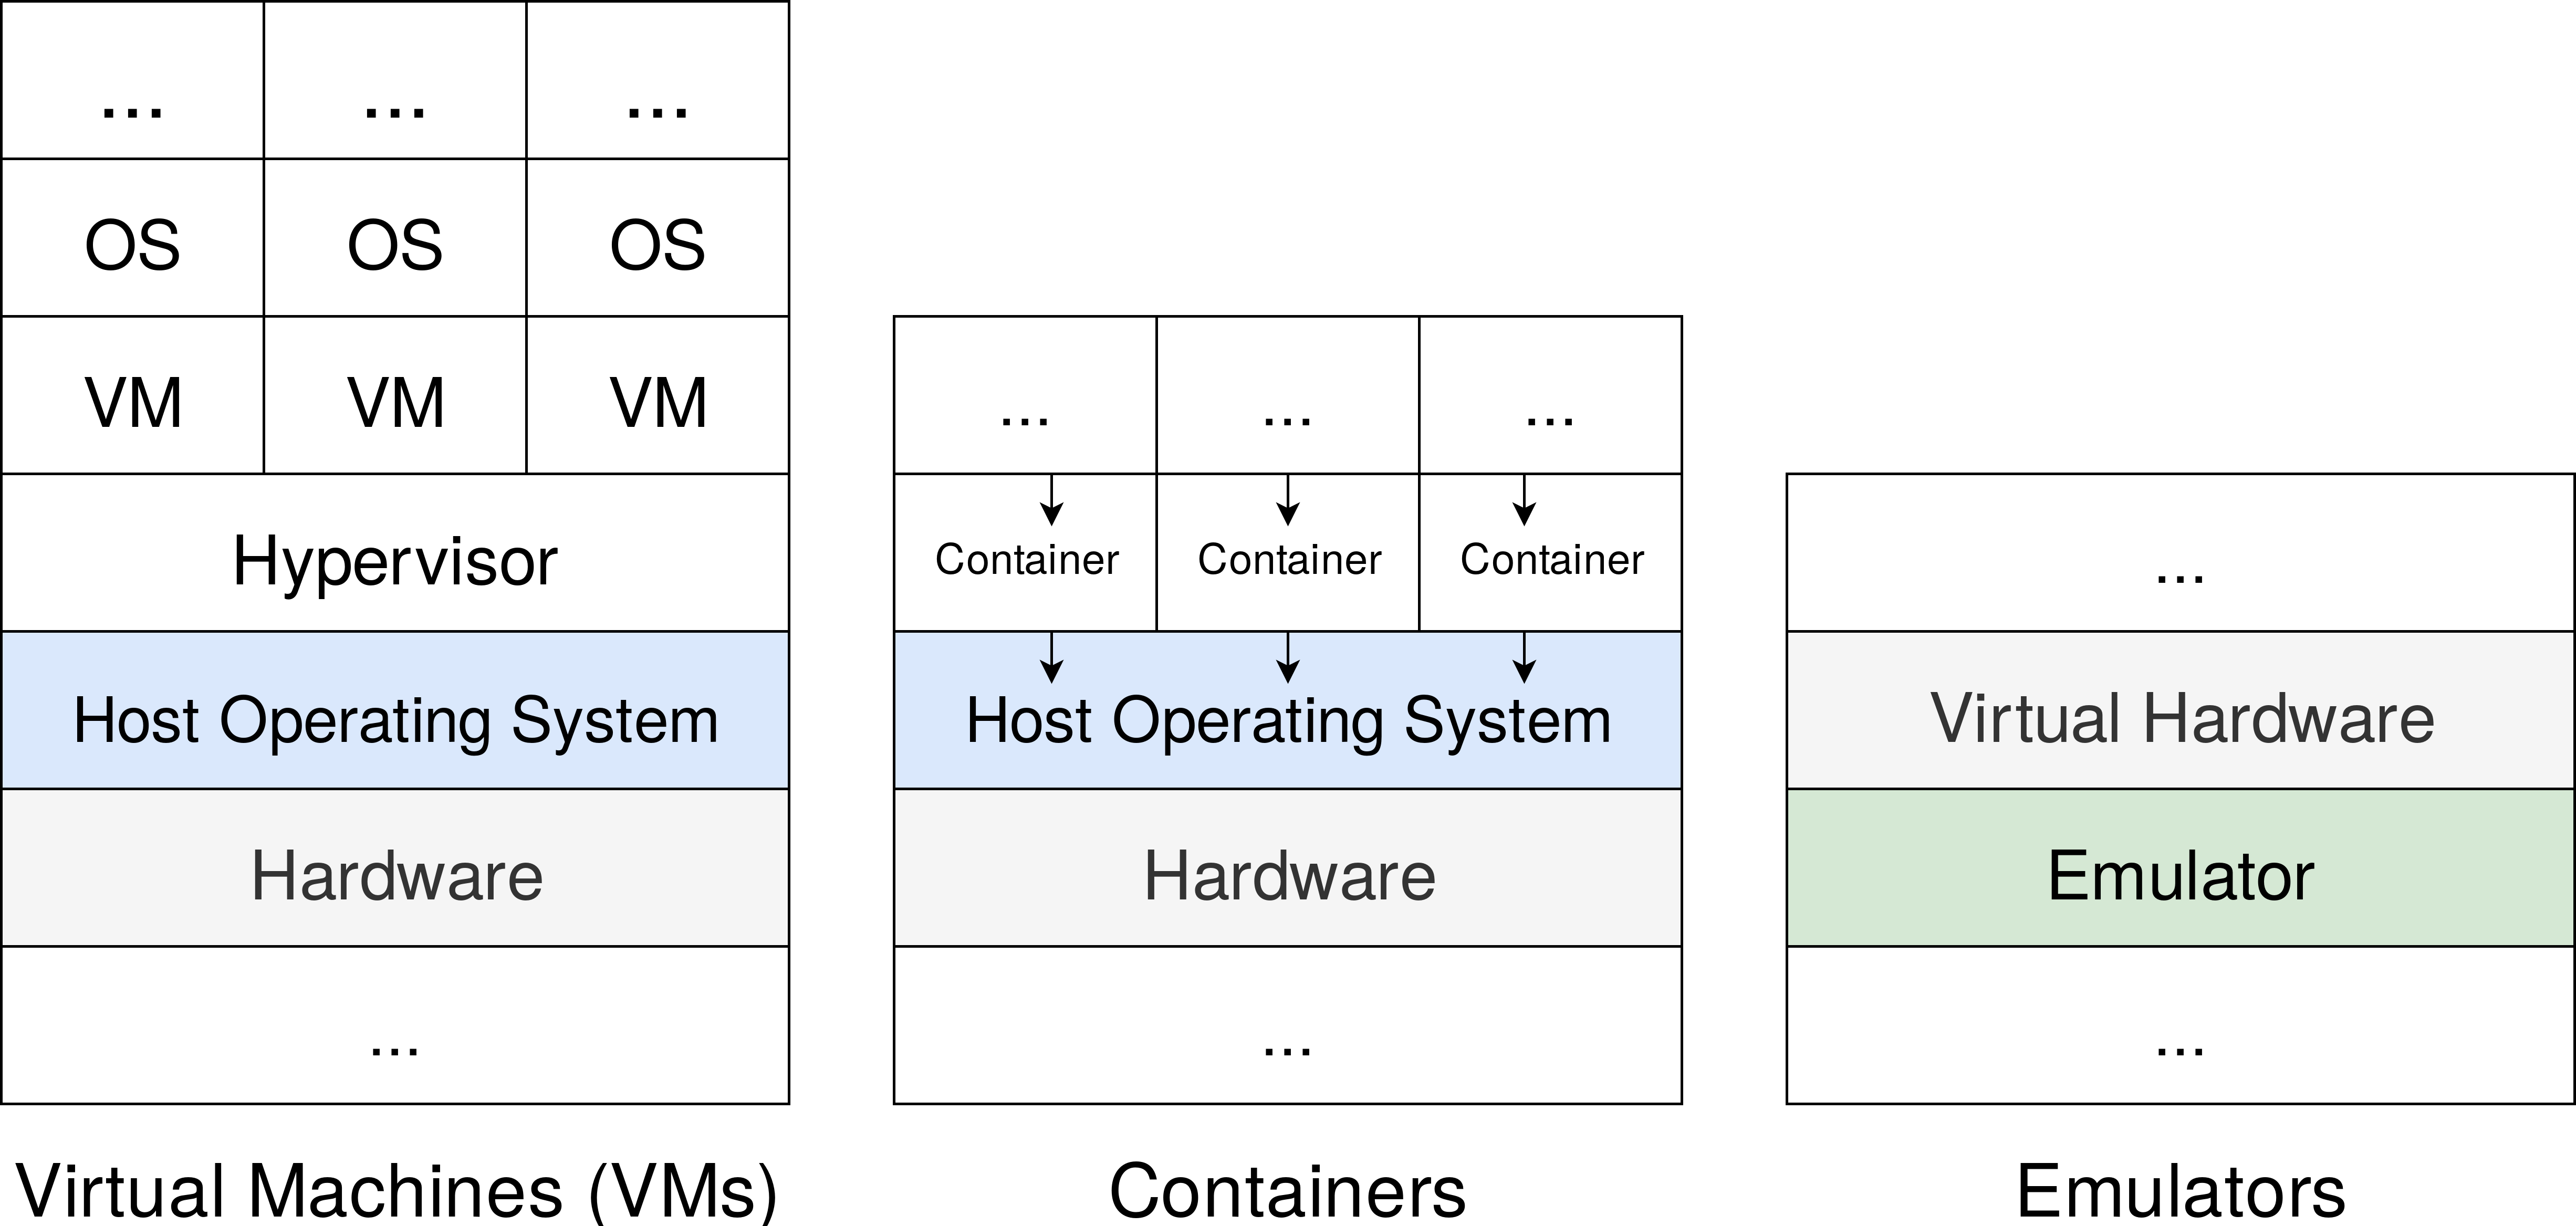
\includegraphics[width=0.70\textwidth]{vms_containers_emulators.png}
    \caption{Virtualization is a very resource expensive proposition. Containerization is cheaper, as it shares a kernel with the host OS. Emulation allows us to emulate hardware as software. Any of these methods can be used in conjunction with any other method.\vspace{-10pt}}
    \label{fig:vms_containers_emulators}
\end{figure}

\section{Containerization}\label{sec:containerization}

One of the challenges of distributed software development across heterogeneous platforms is the problem of variability. With the increasing pace of software development comes the added burden of software maintenance. As hardware and software stacks evolve, so too must source code be updated to build and run correctly. Maintaining a stable and well-documented codebase can be a considerable challenge, especially in an academic setting where contributors are frequently joining and leaving the project. Together, these challenges present significant obstacles to experimental reproducibility and scientific collaboration.


\begin{figure}[ht]
    \centering
    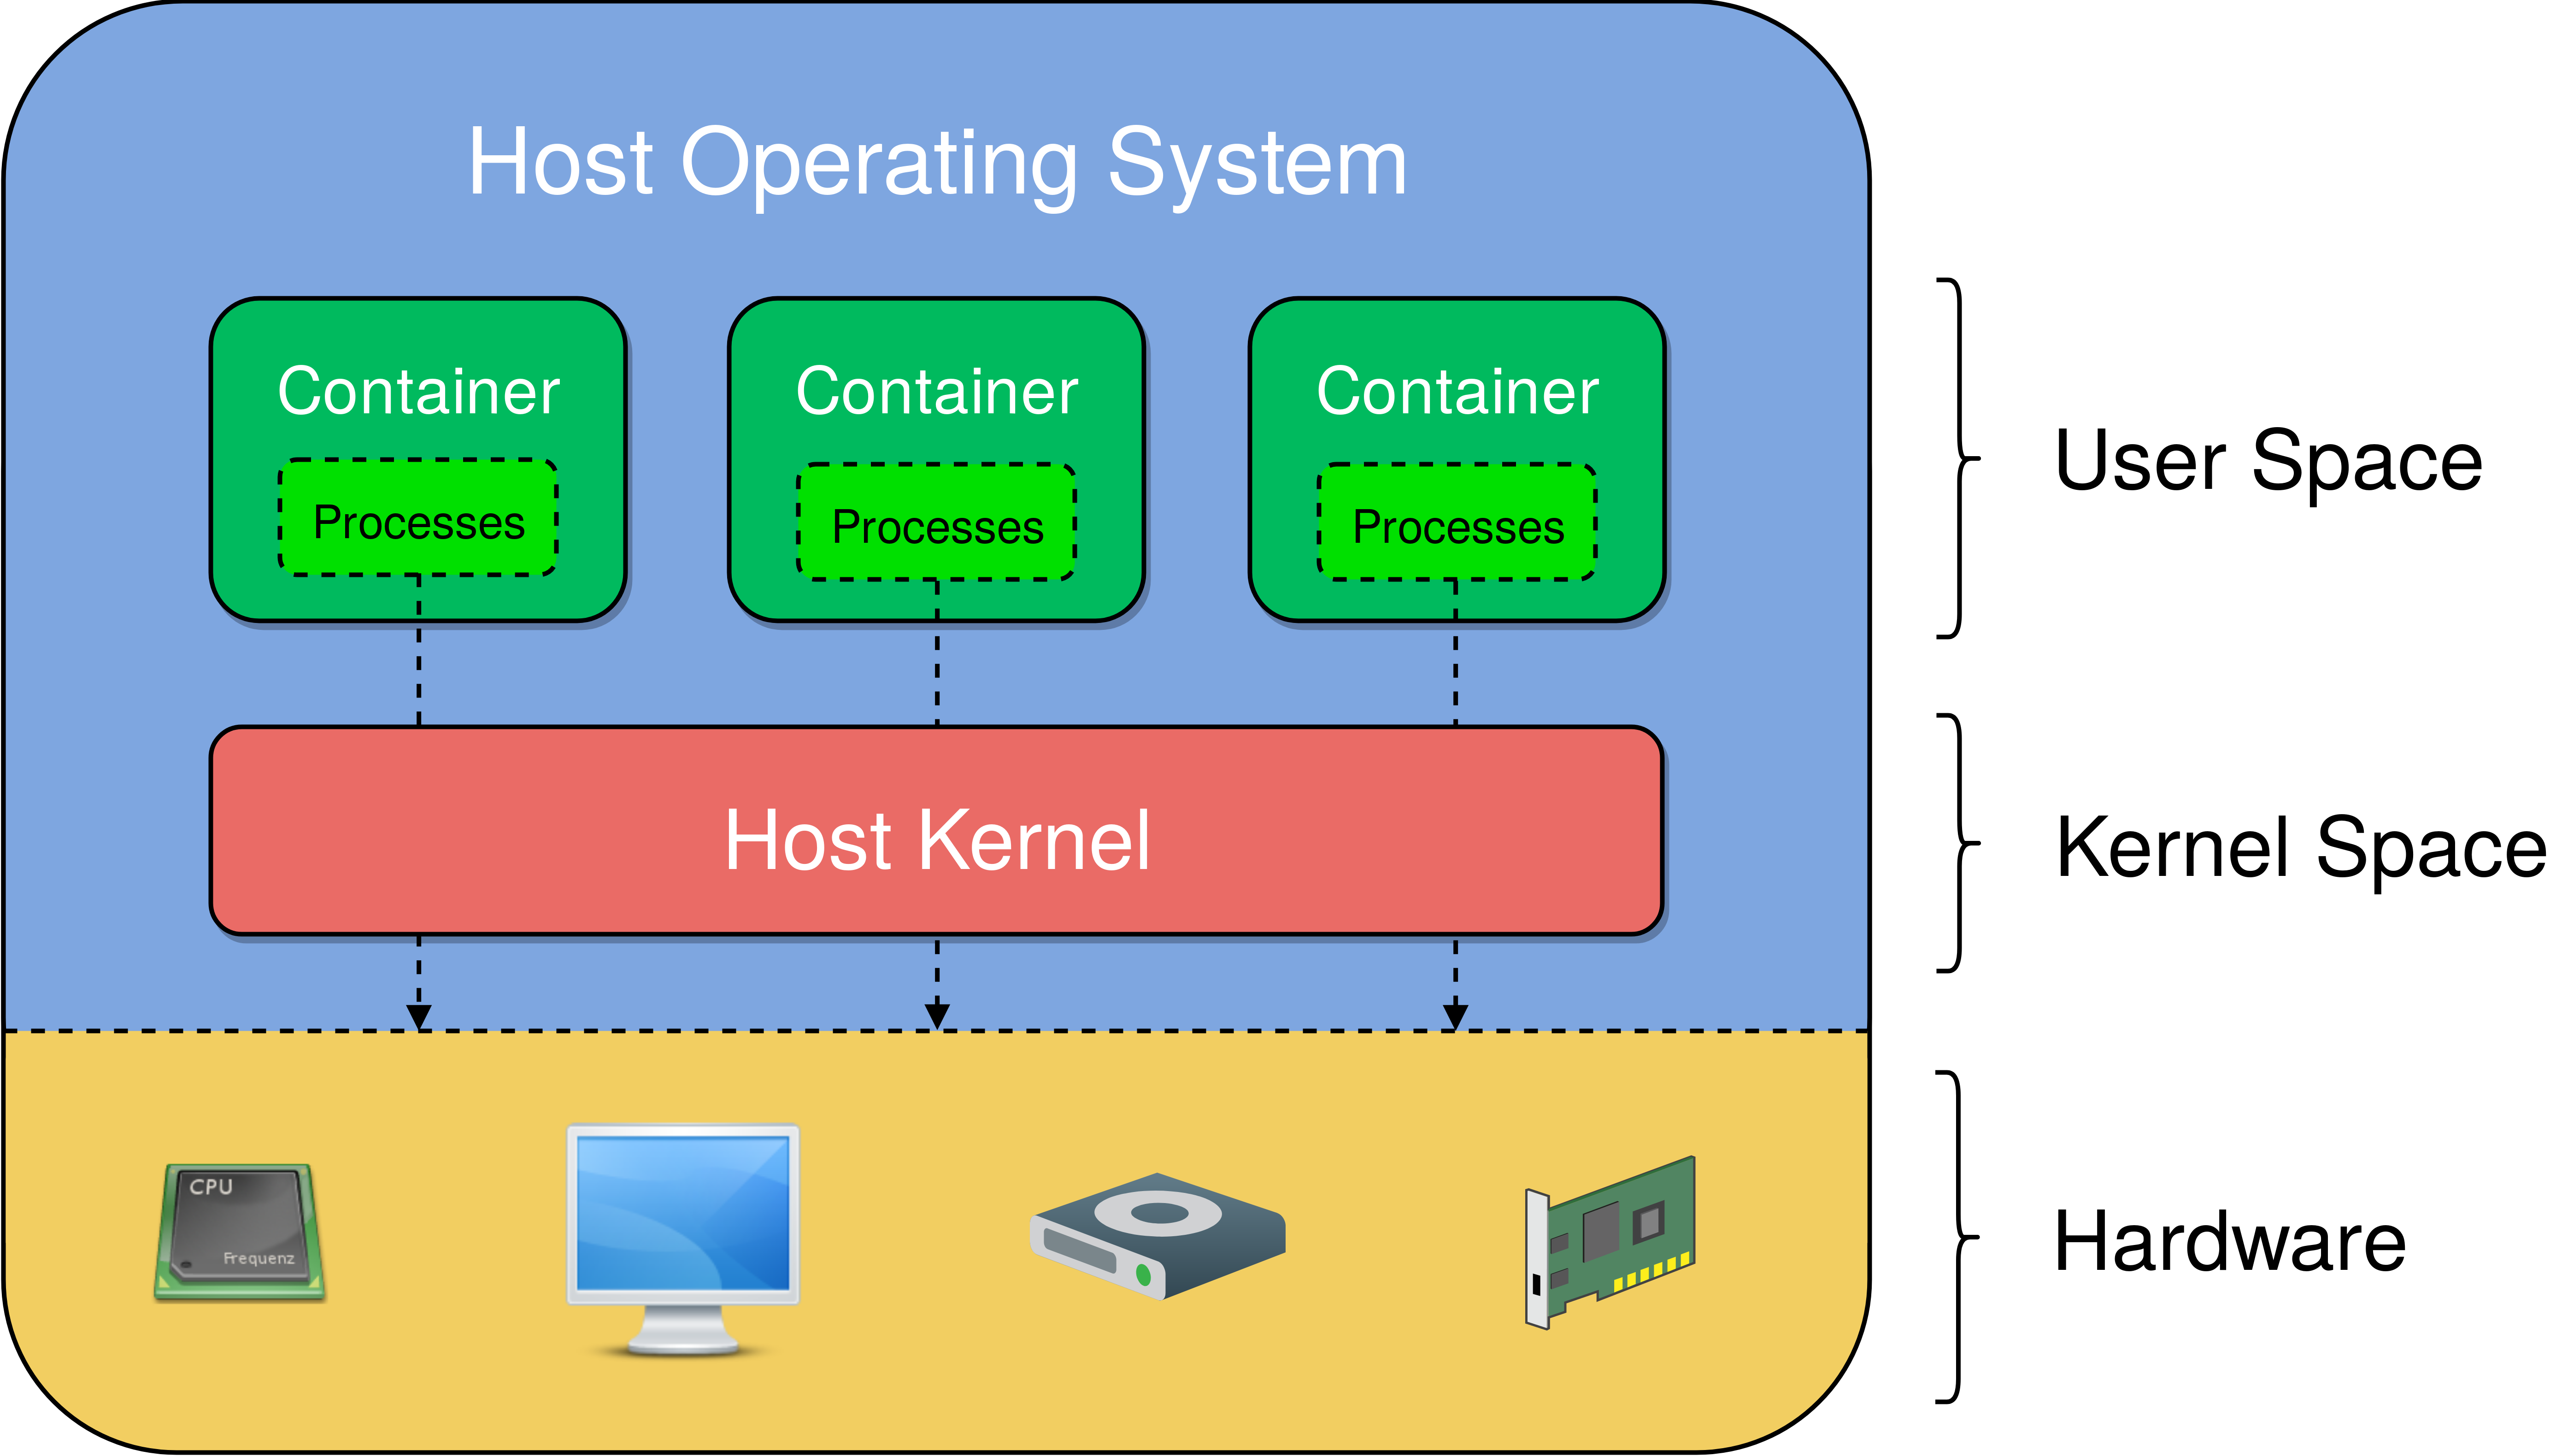
\includegraphics[width=0.65\textwidth]{user_kernel_hardware.png}
    \caption{Containers live in user space. By default they are sandboxed from the host OS and sibling containers, but unlike VMs, share a common kernel with each other and the host OS. All system calls are passed through host kernel.}
    \label{fig:user_kernel_hardware}
\end{figure}

Docker containers are sandboxed runtime environments that are portable, reproducible and version controlled. Each environment contains all the software dependencies necessary to run the packaged application(s), but remains isolated from the host OS and file system. Docker provides a mechanism to control the resources each container is permitted to access, in addition to a separate Linux namespace for each container, effectively isolating the network, users, and file system mounts from the host OS. Unlike virtual machines, container-based virtualization such as Docker only requires a lightweight host, which can support running many simultaneous containers with close to zero overhead compared to native linux processes. A single Raspberry Pi is capable of running hundreds of containers with no noticeable degradation in performance.

While containerization simplifies the process of building and deploying applications considerably, it also introduces some additional complexity to the software development lifecycle. Docker, like most container platforms, uses a layered filesystem. This enables Docker to take an existing ``image'' and change it by installing new dependencies or modifying its functionality. Images may be based on a number of lower layers, which must periodically be updated. Care must be taken when designing the development pipeline to ensure that such updates do not silently break a subsequent layer as described earlier.

\section{Docker Introduction}

Suppose there is a program which is known to run on some computer. It would be nice to give another computer -- any computer with an internet connection -- a short string of ASCII characters, press \keys{\return}, and return to see that program running. Never mind where the program was built or what software happened to be running at the time. This may seem trivial, but is a monumental software engineering problem. Various package managers have attempted to solve this, but even when they work as intended, only support natively compiled binaries on operating systems with the same package manager.

Docker\footnote{The following tutorial uses Docker, but the workflow described is similar to most container platforms.} is a tool for portable, reproducible computing. With Docker, users can run any Linux program on almost any networked computing device on the planet, regardless of the underling operating system or hardware architecture. All of the environment preparation, installation and configuration steps can be automated from start to finish. Depending on how much network bandwidth is available, it might take some time, but users will never need to intervene in the installation process.

To install Docker itself, execute the following command on a POSIX-compliant shell of any Docker-supported platform:

\begin{pclisting}
~$ curl -sSL https://get.docker.com/ | sh
\end{pclisting}

A Docker \textit{image} is basically a filesystem snapshot -- a single file that contains everything needed to run a certain Docker container. Docker images are hosted in \textit{registries}, similar to Git repositories or VCS servers. The following command will fetch a Docker image, e.g. \inline{daphne/duck} from the default Docker Hub repository:

\begin{pclisting}
~$ docker pull daphne/duck
\end{pclisting}

Every Docker image has a image ID, a name and a tag:

\begin{pclisting}
~$ docker images
REPOSITORY      TAG        IMAGE ID         CREATED       SIZE
daphne/duck     latest     ea2f90g8de9e     1 day ago     869MB
\end{pclisting}

To run a Docker container\footnote{When a Docker image is running, it is referred to as a \textit{container}.}, use the following command:

\begin{pclisting}
~$ docker run daphne/duck
\end{pclisting}

The following command will verify the container is indeed running:

\begin{pclisting}
~$ docker ps
CONTAINER ID     IMAGE           ...     NAMES
52994ef22481     daphne/duck     ...     happy_hamster
\end{pclisting}

Note how Daphne's duck container has an alphanumeric container ID, a base image, and a memorable name, \inline{happy_hamster}. This name is an alias for the container ID, which can be used interchangeably to refer to the container.

Docker images can be created two different ways. In \autoref{subsec:creating-an-image-snapshot}, we will see how to create a Docker image by taking a snapshot from a running container, then in \autoref{subsec:writing-an-image-recipe}, how to create a new Docker container using a special kind of recipe, called a \inline{Dockerfile}.

\subsection{Creating an image snapshot}\label{subsec:creating-an-image-snapshot}

When a Docker container writes to its own filesystem, those changes are not persisted unless committed to a new image. For example, start a container with an interactive shell:

\begin{pclisting}
~$ docker run -it daphne/duck bash
root@295fd7879184:/#
\end{pclisting}

Note the container ID: \inline{295fd7879184}. If we write to disk and leave the container,

\begin{pclisting}
root@295fd7879184:/# touch new_file && ls -l
total 0
-rw-r--r-- 1 root root 0 May 21 20:52 new_file
root@295fd7879184:/# exit
\end{pclisting}

\inline{new_file} will not be persisted. If we re-run the same command again:

\begin{pclisting}
~$ docker run -it daphne/duck bash
root@18f13bb4571a:/# ls
root@18f13bb4571a:/# touch new_file1 && ls -l
total 0
-rw-r--r-- 1 root root 0 May 21 21:32 new_file1
\end{pclisting}

It seems like \inline{new_file} has disappeared! Notice how the container ID (\inline{18f13bb4571a}) is now different. This is because the command \inline{docker run daphne/duck} created a new container from the base image \inline{daphne/duck}, rather than restarting the previous container.

To see all containers on a Docker host, run the following command:

\begin{pclisting}
~$ docker container ls -a
CONTAINER ID      IMAGE            STATUS             NAMES
295fd7879184      daphne/duck      Exited (130)       merry_manatee
18f13bb4571a      daphne/duck      Up 5 minutes       shady_giraffe
52994ef22481      daphne/duck      Up 10 minutes      happy_hamster
\end{pclisting}

It appears \inline{295fd7879184} a.k.a. \inline{merry_manatee} survived, but it is no longer running. Whenever a container's main process (recall we ran \inline{merry_manatee} with \inline{bash}) finishes, the container will stop, but it will not cease to exist. In fact, we can resume the stopped container right where it left off:

\begin{pclisting}
~$ docker start -a merry_manatee
root@295fd7879184:/# ls -l
total 0
-rw-r--r-- 1 root root 0 May 21 20:52 new_file
\end{pclisting}

Nothing was lost! To verify this, we can check which other containers are running:

\begin{pclisting}
~$ docker ps
CONTAINER ID       IMAGE             ...       NAMES
295fd7879184       daphne/duck       ...       merry_manatee
18f13bb4571a       daphne/duck       ...       shady_giraffe
52994ef22481       daphne/duck       ...       happy_hamster
\end{pclisting}

Now suppose we would like to share the container \inline{shady_giraffe} with someone else. To do so, we must first snapshot the running container, or commit it to a new image with a name and a tag. This will create a checkpoint that we may later restore:

\begin{pclisting}
~$ docker commit -m "forking daphne/duck" shady_giraffe user/duck:v2
\end{pclisting}

To refer to the container, we can either use \inline{18f13bb4571a} or the designated name (i.e. \inline{shady_giraffe}). This image repository will be called \inline{user/duck}, and has an optional version identifier, \inline{:v2}, which can be pushed to the Docker Hub registry:

\begin{pclisting}
~$ docker push user/duck:v2
~$ docker images
REPOSITORY    TAG        IMAGE ID         CREATED          SIZE
daphne/duck   latest     ea2f90g8de9e     1 day ago        869MB
user/duck     v2         d78be5cf073e     2 seconds ago    869MB
~$ docker pull user/duck:v2
~$ docker run user/duck ls -l
total 0
-rw-r--r-- 1 root root 0 May 21 21:32 new_file1
\end{pclisting}

This is a convenient way to share an image with colleagues and collaborators. Anyone with access to the repository can pull this image and continue where we left off, or create another image based on top.

\subsection{Writing an image recipe}\label{subsec:writing-an-image-recipe}

The second way to create a Docker image is to write a recipe, called a \inline{Dockerfile}. A \inline{Dockerfile} is a text file that specifies the commands required to create a Docker image, typically by modifying an existing container image using a scripting interface. They also have special keywords (which are conventionally \inline{CAPITALIZED}), like \inline{FROM}, \inline{RUN}, \inline{ENTRYPOINT} and so on. For example, create a file called \inline{Dockerfile} with the following content:

\begin{dockerlisting}
FROM daphne/duck      # Defines the base image
RUN touch new_file1   # new_file1 will be part of our snapshot
CMD ls -l             # Default command run when container is started
\end{dockerlisting}

Now, to build the image, we can simply run:

\begin{pclisting}
~$ docker build -t user/duck:v3 .
\end{pclisting}

The `\inline{.}' indicates the same directory as the \inline{Dockerfile}. This should produce something like the following output:

\begin{pclisting}
Sending build context to Docker daemon  2.048kB
Step 1/3 : FROM daphne/duck
--- ea2f90g8de9e
Step 2/3 : RUN touch new_file1
--- e3b75gt9zyc4
Step 3/3 : CMD ls -l
--- Running in 14f834yud59
Removing intermediate container 14f834yud59
--- 05a3bd381fc2
Successfully built 05a3bd381fc2
Successfully tagged user/duck:v3
\end{pclisting}

The command, \inline{docker images} should display an image called \inline{user/duck:v3}:

\begin{pclisting}
~$ docker images
REPOSITORY    TAG        IMAGE ID         CREATED          SIZE
daphne/duck   latest     ea2f90g8de9e     1 day ago        869MB
user/duck     v2         d78be5cf073e     5 minutes ago    869MB
user/duck     v3         05a3bd381fc2     2 seconds ago    869MB
\end{pclisting}

This procedure is identical to the snapshot technique performed in \autoref{subsec:creating-an-image-snapshot}, but the result is cleaner. Rather than maintaining a 869 MB image, we can just store the 4 KB text file instead. To run the resulting image, we can simply use the same command as before:

\begin{pclisting}
~$ docker run -it user/duck:v3
total 0
-rw-r--r-- 1 root root 0 May 21 21:35 new_file1
\end{pclisting}

Notice that as soon as we run the container, Docker will execute the \inline{ls -l} command as specified by the \inline{Dockerfile}, revealing that \inline{new_file1} was indeed stored in the image. However this default command can be overridden by supplying a custom command:

\begin{pclisting}
~$ docker run -it user/duck:v3 [custom_command]
\end{pclisting}

\subsection{Layer Caching}

An important concept in Docker is the concept of layers. One way to think of a layer is like a Git commit -- a set of changes to a previous image or layer, identified by a hash code. In a \inline{Dockerfile}, layers begin with a keyword.

\begin{dockerlisting}
FROM daphne/duck
RUN touch new_file1                            # Defines a new layer
RUN mkdir config && mv new_file1 mkdir         # Layers can chain commands
RUN apt-get update && apt-get install -y wget  # Install a dependency
RUN wget https://get.your.app/install.sh       # Download a script
RUN chmod +x install.sh && ./install.sh        # Run the script
\end{dockerlisting}

To build this image, we can run the following command:

\begin{pclisting}
~$ docker build -t user/duck:v4 .
Sending build context to Docker daemon  2.048kB
Step 1/6 : FROM daphne/duck
---> cd6d8154f1e1
...
Removing intermediate container 8fb56ef38bc8
---> 3358ca1b8649
Step 5/6 : RUN wget https://get.your.app/install.sh
---> Running in e8284ff4ec8b
...
2018-10-30 06:47:57 (89.9 MB/s) - 'install.sh' saved [13847/13847]
Removing intermediate container e8284ff4ec8b
---> 24a22dc2900a
Step 6/6 : RUN chmod +x install.sh && ./install.sh
---> Running in 9526651fa492
# Executing install script, commit: 36b78b2
...
Removing intermediate container 9526651fa492
---> a8be23fea573
Successfully built a8be23fea573
Successfully tagged user/duck:v4
\end{pclisting}

Layers are conveniently cached by the Docker daemon. If we run the same command again, Docker will use the cache insead of rebuilding the entire image:

\begin{pclisting}
Sending build context to Docker daemon  2.048kB
Step 1/6 : FROM daphne/duck
---> cd6d8154f1e1
Step 2/6 : RUN touch new_file1
---> Using cache
---> 0473154b2004
...
Step 6/6 : RUN chmod +x index.html && ./index.html
---> Using cache
---> a8be23fea573
Successfully built a8be23fea573
Successfully tagged user/duck:v4
\end{pclisting}

Should we later need to make a change to the Dockerfile, Docker will only rebuild the image starting from the first modified step. Suppose we add a new \inline{RUN} command to the end of our \inline{Dockerfile} and trigger a rebuild like so:

\begin{pclisting}
~$ echo 'RUN echo "Change here!"' >> Dockerfile
~$ docker build -t user/duck:v4 .
Sending build context to Docker daemon  2.048kB
...
Step 6/7 : RUN chmod +x index.html && ./index.html
---> Using cache
---> a8be23fea573
Step 7/7 : RUN echo "Change here!"
---> Running in 80fc5c402304
Change here!
Removing intermediate container 80fc5c402304
---> c1ec64cef9c6
Successfully built c1ec64cef9c6
Successfully tagged user/duck:v4
\end{pclisting}

If Docker had to rerun the entire \inline{Dockerfile} from top to bottom to every time it was rebuilt, this would be slow and inconvenient. Instead, Docker caches the unmodified steps by default, and only reruns the minimum set of steps necessary to rebuild. This can sometimes introduce unexpected results, especially when the cache is stale. To ignore the cache and force a clean rebuild, use the \inline{--no-cache} flag when building a \inline{Dockerfile}.

What does Docker consider when deciding whether to use the cache? First is the \inline{Dockerfile} itself -- when a step in a \inline{Dockerfile} changes, both it and any subsequent steps will need to be rerun during a build. Docker also considers the build context. When ``\inline{docker build -t TAG .}'' is written, the `\inline{.}' indicates the context, or path where the build should occur. Often, this path contains build artifacts. For example:

\begin{dockerlisting}
FROM daphne/duck
COPY duck.txt .
RUN cat duck.txt
\end{dockerlisting}

Now if we add some message in \inline{duck.txt} and rebuild our image, the file will be copied into the Docker image, and its contents will be printed:

\begin{pclisting}
~$ echo "Make way!" > duck.txt && docker build -t user/duck:v5 .
Sending build context to Docker daemon  3.072kB
Step 1/3 : FROM daphne/duck
---> cd6d8154f1e1
Step 2/3 : COPY duck.txt .
---> e0e03d9e1791
Step 3/3 : RUN cat duck.txt
---> Running in 590c5420ce29
Make way!
Removing intermediate container 590c5420ce29
---> 1633e3e10bef
Successfully built 1633e3e10bef
Successfully tagged user/duck:v5
\end{pclisting}

As long as the first three lines of the \inline{Dockerfile} and \inline{duck.txt} are not modified, these layers will be cached and Docker will not need to rebuild them. However if the contents of the file \inline{duck.txt} are subsequently modified, this will force a rebuild to occur. For example, if we append to the file and rebuild, only the last step will be executed:

\begin{pclisting}
~$ echo "Thank you. Have a nice day!" >> duck.txt
~$ docker build -t user/duck:v5 .
Sending build context to Docker daemon  3.072kB
Step 1/3 : FROM ubuntu
---> cd6d8154f1e1
Step 2/3 : COPY duck.txt .
---> f219efc150a5
Step 3/3 : RUN cat duck.txt
---> Running in 7c6f5f8b73e9
Make way!
Thank you. Have a nice day!
Removing intermediate container 7c6f5f8b73e9
---> e8a1db712aee
Successfully built e8a1db712aee
Successfully tagged user/duck:v5
\end{pclisting}

A common mistake when writing \inline{Dockerfile}s is to \inline{COPY} more files than are strictly necessary to perform the following build step. For example, if \inline{COPY . .} is written at the beginning of the \inline{Dockerfile}, whenever a file in changed anywhere in the build context, this will trigger a rebuild of all subsequent build steps. In order to maximize cache reusability and minimize rebuild time, users should be conservative and only \inline{COPY} the minimum set of files necessary to accomplish the following build step.

% Like Git's \inline{.gitignore}, Docker also has a \inline{.dockerignore} file. If we add a line to the \inline{.dockerignore} file, then all paths matching this line in the build context will be ignored. Docker also accepts other patterns like regular expressions and negation.~\footnote{Further details: \url{https://docs.docker.com/engine/reference/builder/#dockerignore-file}}

\subsection{Volume Sharing}\label{subsec:volume_sharing}

There is a second method of depositing data into a container, which does not require baking it into the parent image at compile time. This method is more appropriate for data which is required at runtime, but non-essential for the build. It takes the following form:

\begin{pclisting}
~$ docker run user/duck:v6 -v [host_volume]:[target_volume]
\end{pclisting}

Suppose we have a \inline{Dockerfile} which provides a default \inline{CMD} instruction:

\begin{dockerlisting}
FROM daphne/duck
CMD /bin/bash -c "/launch.sh"
\end{dockerlisting}

If we built this image and tried to run it, the file \inline{launch.sh} would be missing:

\begin{pclisting}
~$ docker build -t user/duck:v6 && docker run user/duck:v6
bash: /launch.sh: No such file or directory
\end{pclisting}

Instead, when running the container, we need to share the file via the Docker CLI:

\begin{pclisting}
~$ echo -e '#!/bin/bash\necho Launching...' >> launch.sh && \
   chmod 775 launch.sh && \
   docker run user/duck:v6 -v launch.sh:/launch.sh
Launching...
\end{pclisting}

This way, the local file \inline{launch.sh} will be available to use from within the container at the designated path, \inline{/launch.sh}.

\subsection{Multi-stage builds}

Docker's filesystem is additive, so each layer will only increase the size of the final image. For this reason, it is often necessary to tidy up unneeded files after installation. For example, when installing dependencies on Debian-based images, it is a common practice to run:

\begin{dockerlisting}
RUN apt-get update && apt-get install ... && rm -rf /var/lib/apt/lists/*
\end{dockerlisting}

This ensures the package list is not baked into the image (Docker will only checkpoint the layer after each step is complete). Builds can often take several steps, despite only producing a single artifact. Instead of chaining together several commands and cleaning up changes in a single step, multi-stage builds let us build a series of images inside a \inline{Dockerfile}, and copy resources from one to another, discarding all intermediate build artifacts:

\begin{dockerlisting}
FROM user/duck:v3 as template1

FROM daphne/duck as template2
COPY --from=template1 new_file1 new_file2
FROM donald/duck as template3
COPY --from=template2 new_file2 new_file3
CMD ls -l
\end{dockerlisting}

Now we can build and run this image as follows:

\begin{pclisting}
~$ docker build . -t user/duck:v4
Sending build context to Docker daemon  2.048kB
Step 1/6 : FROM user/duck:v3 as template1
--- e3b75ef8ecc4
Step 2/6 : FROM daphne/duck as template2
--- ea2f90g8de9e
Step 3/6 : COPY --from=template1 new_file1 new_file2
---> 72b96668378e
Step 4/6 : FROM donald/duck:v3 as template3
---> e3b75ef8ecc4
Step 5/6 : COPY --from=template2 new_file2 new_file3
---> cb1b84277228
Step 6/6 : CMD ls
---> Running in cb1b84277228
Removing intermediate container cb1b84277228
---> c7dc5dd63e77
Successfully built c7dc5dd63e77
Successfully tagged user/duck:v4
~$ docker run -it user/duck:v4
total 0
-rw-r--r-- 1 root root 0 Jul  8 15:06 new_file3
\end{pclisting}

One application of multi-stage builds is compiling a project dependency from its source code. In addition to all the source code, the compilation process could introduce gigabytes of build artifacts and transitive dependencies, just to build a single binary. Multi-stage builds allow us to build the file, and copy it to a fresh layer, unburdened by intermediate files.

\section{ROS and Docker}

\begin{figure}[ht]
    \centering
    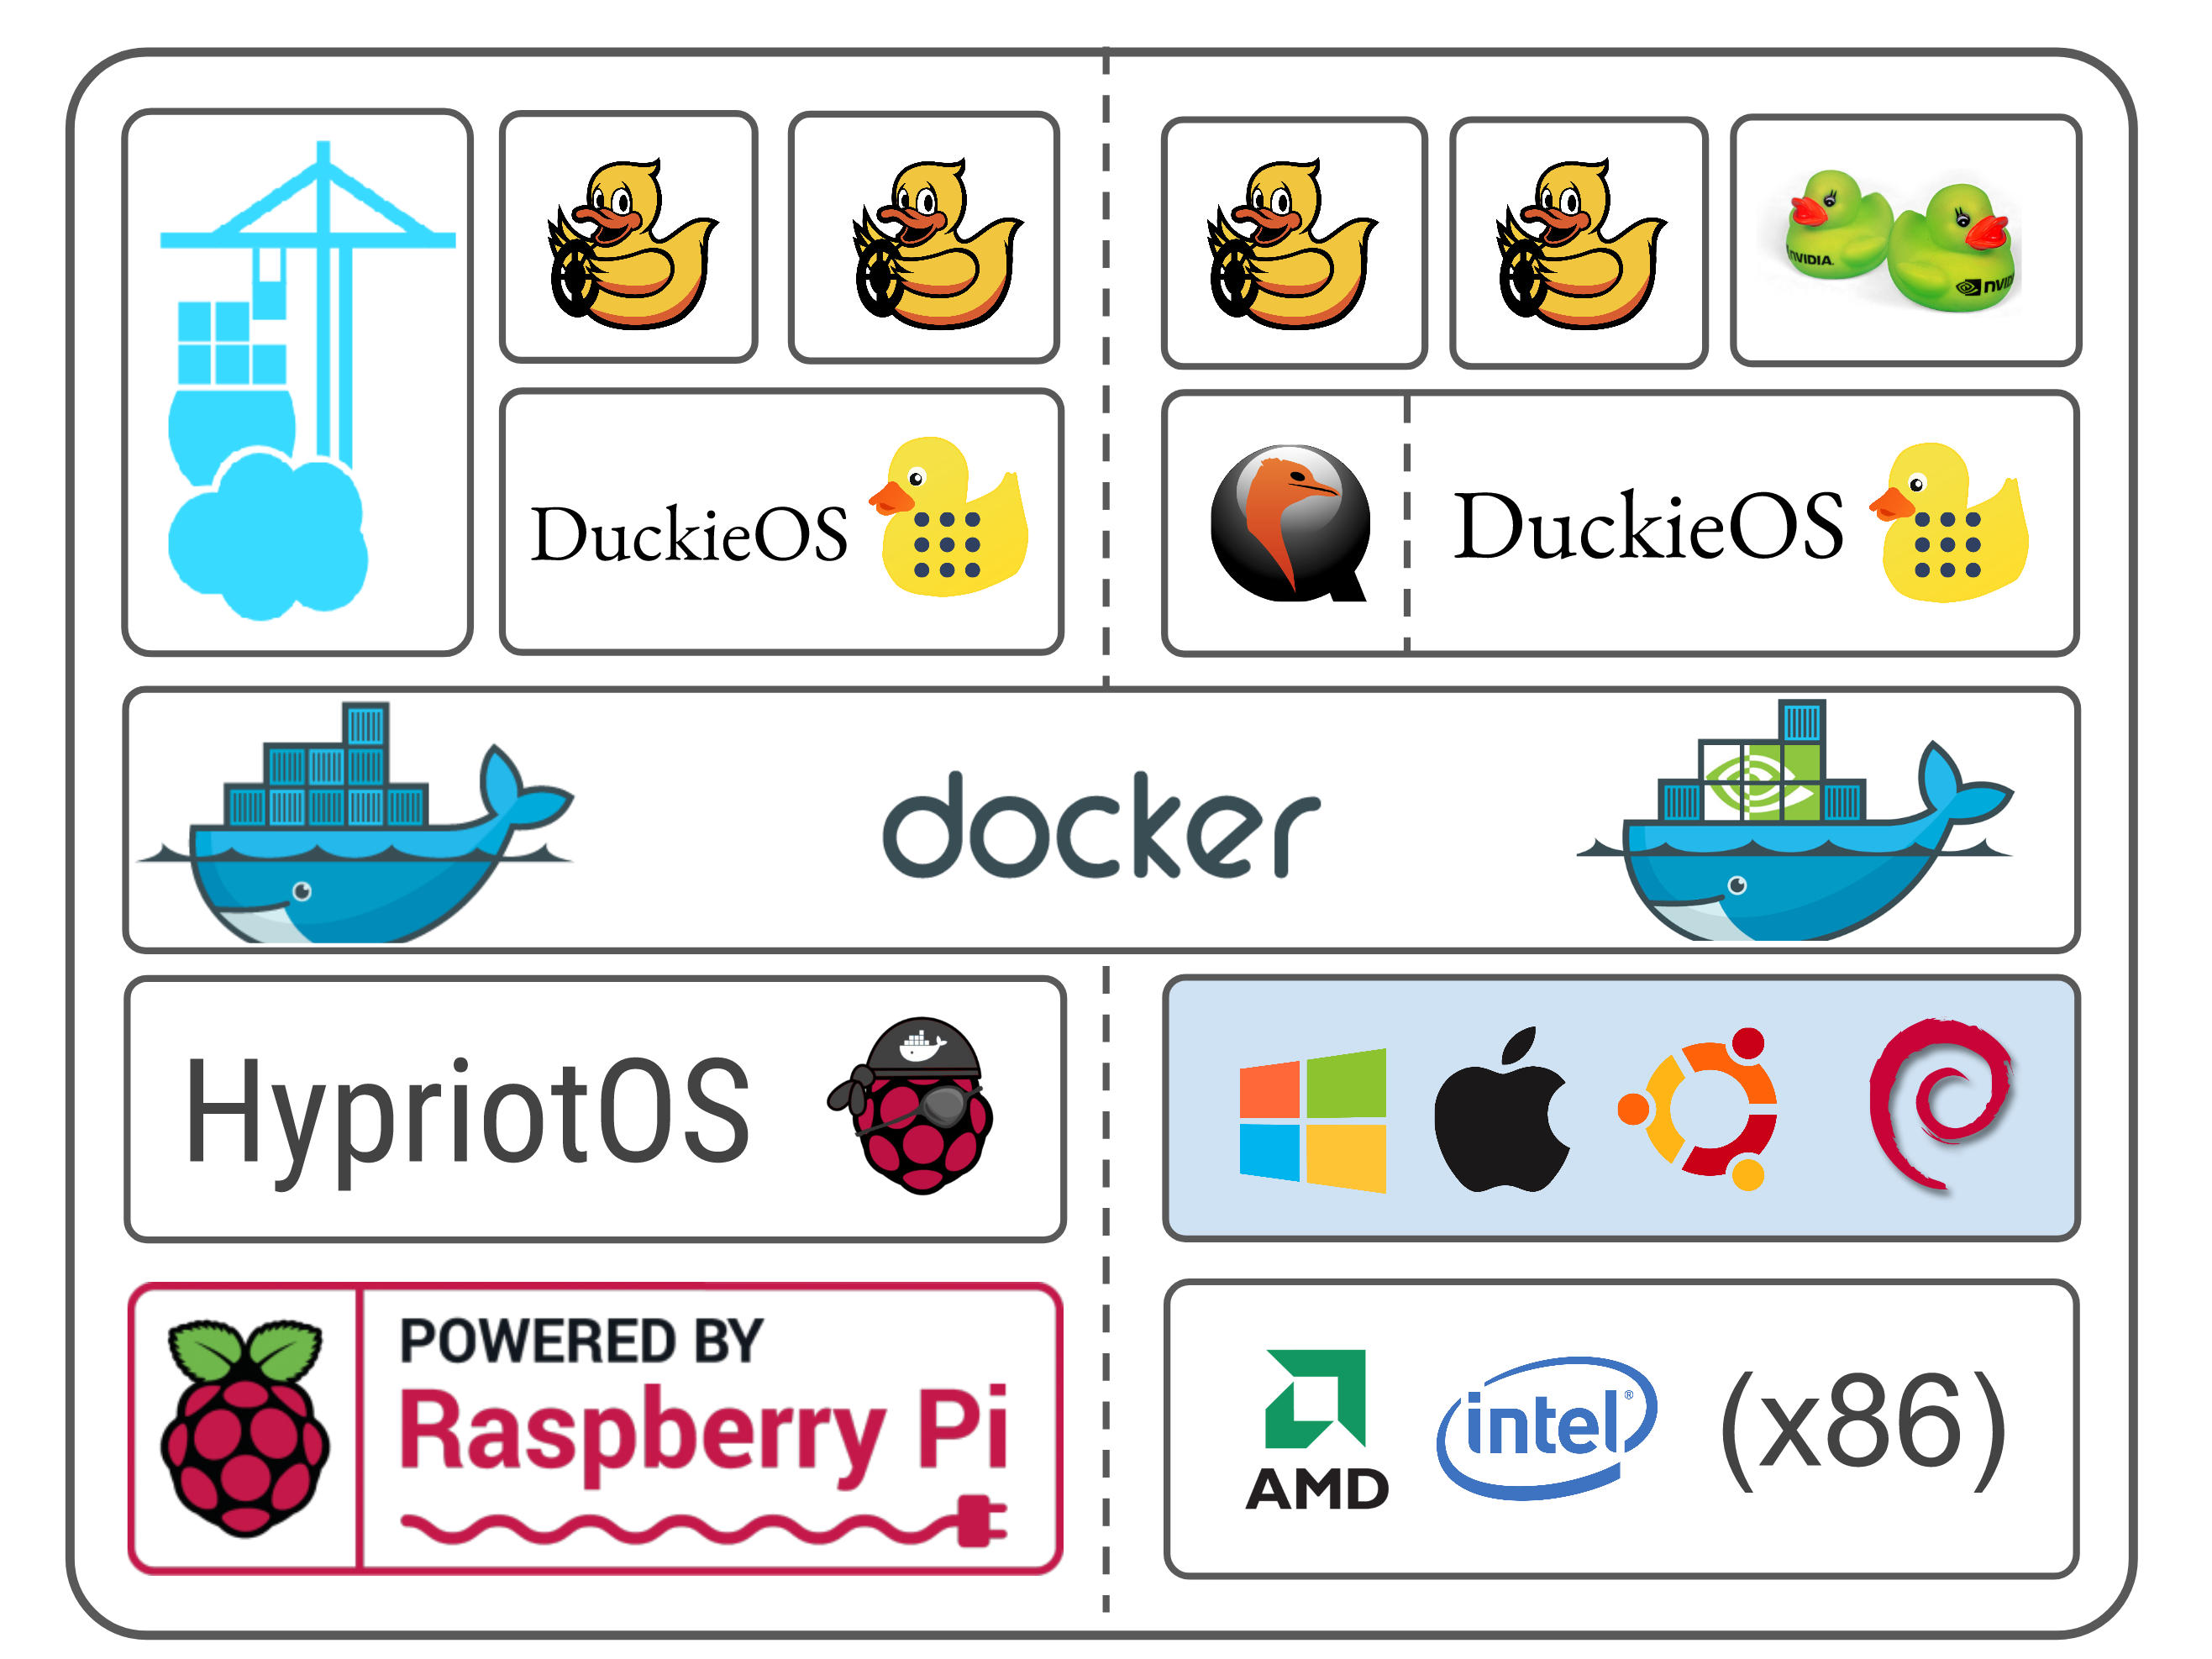
\includegraphics[width=0.48\textwidth]{docker_stack_1.png}
    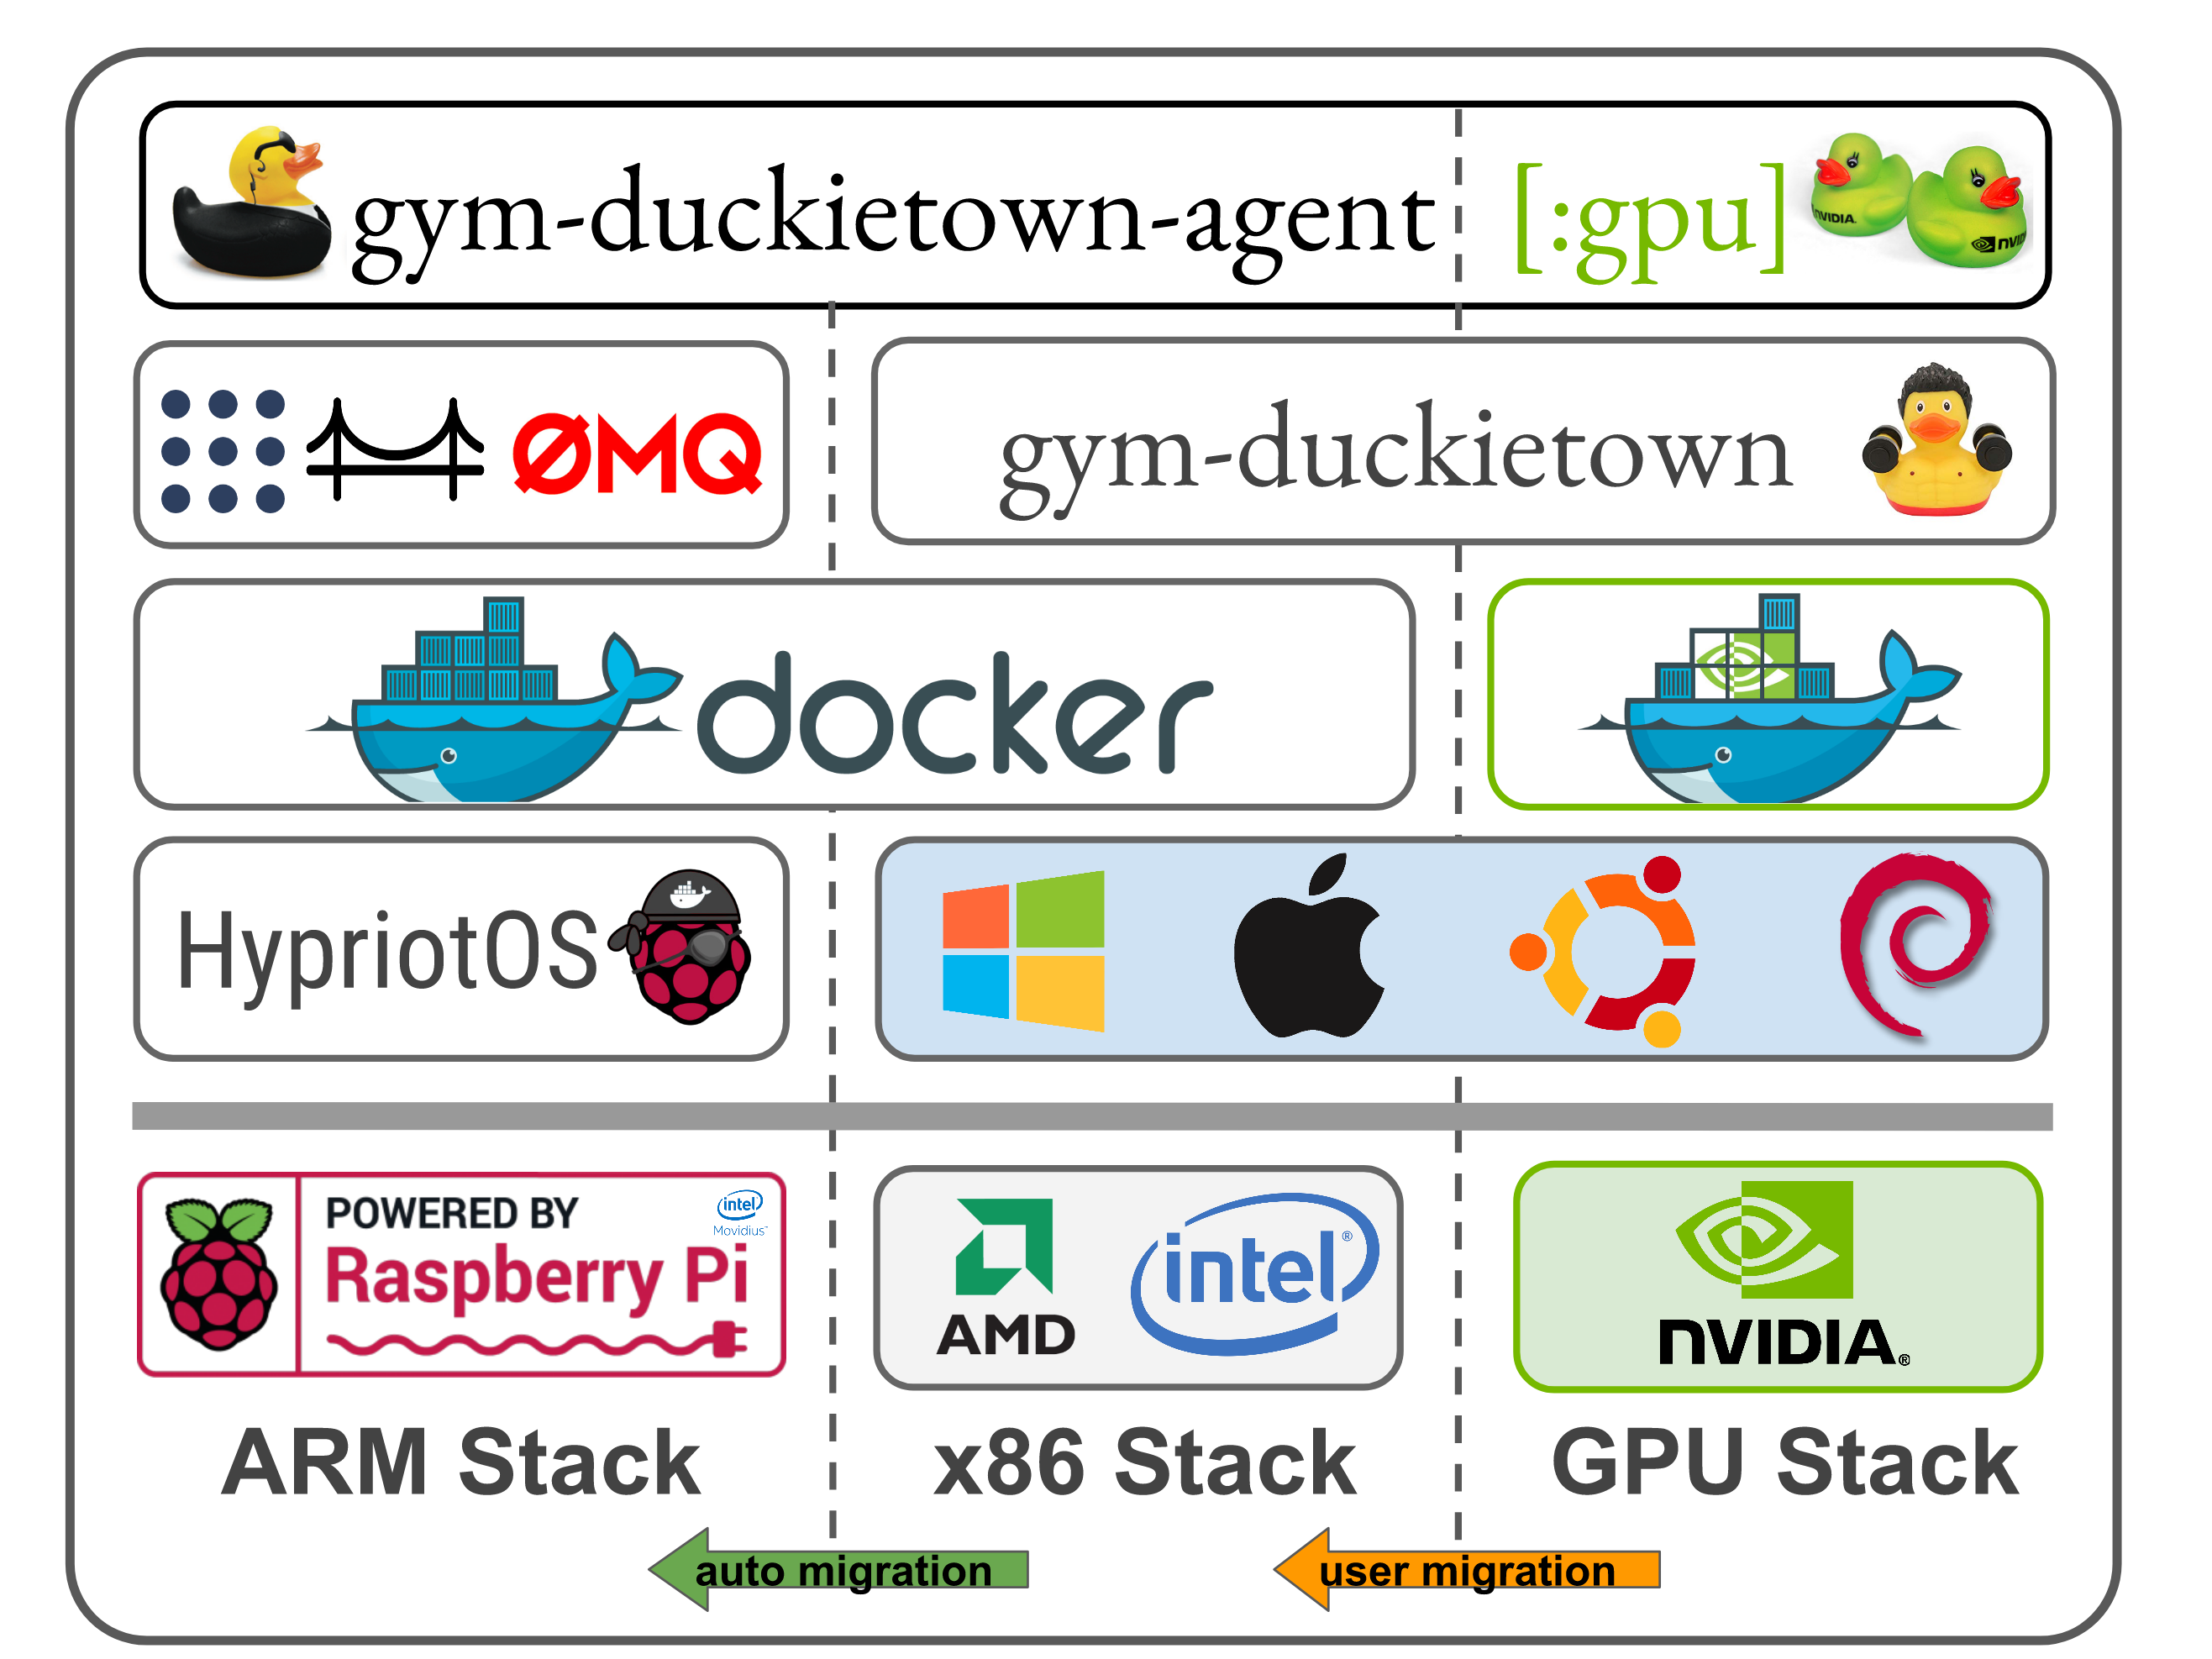
\includegraphics[width=0.48\textwidth]{docker_stack_2.png}
    \caption{Container infrastructure. \textbf{Left}: The ROS stack targets two primary architectures, x86 and ARM. To simplify the build process, we only build ARM artifacts, and emulate ARM on x86. \textbf{Right}: Reinforcement learning stack. Build artifacts are trained on a GPU, and transferred to CPU for evaluation. Deep learning models, depending on their architecture, may be run on an ARM device using an accelerator.}
    \label{fig:docker}
\end{figure}

Prior work has explored the Dockerization of ROS containers~\citep{white2017ros-docker}. This work forms the basis for our own, which extends White and Christensen's work to the Duckietown platform~\citep{paull2017duckietown}, which is more hardware- and domain-specific.

The Duckietown platform supports two primary instruction set architectures: x86 and ARM. To ensure the runtime compatibility of Duckietown packages, we cross-build using hardware virtualization to ensure build artifacts can be run on either target architecture. Runtime emulation of foreign artifacts is also possible, using a similar technique.\footnote{For more information, this technique is described in further depth at the following URL: \url{https://www.balena.io/blog/building-arm-containers-on-any-x86-machine-even-dockerhub/}.} For performance and simplicity, we only use emulation where necessary (e.g., on x86 devices). On ARM-native, the base operating system is HypriotOS, a lightweight Debian distribution for the Raspberry Pi and other ARM-based SBCs, with native support for Docker. For both x86 and ARM-native, Docker is the underlying container platform upon which all user applications are run, inside a container. Since both ROS and Docker have extensive command line interfaces, we provide a unified interface, the Duckietown Shell (\inline{dts}), which wraps their functionality and runs common tasks.

\section{Duckiebot Development using Docker}

Software development for the Duckietown platform requires the following physical objects:
%
\begin{enumerate}
    \item Duckiebot (including custom hat, camera, wheels, and Raspberry Pi 3B+)\footnote{Full materials list can be located at the following URL: \url{https://get.duckietown.org/}}
    \item Micro SD card (16GB+ recommended)
    \item Personal computer
    \item Internet-enabled router
    \item MicroSD card adapter
\end{enumerate}
%
Furthermore, we assume the following software dependencies have been installed on (3):
%
\begin{enumerate}[label=(\alph*)]
    \item Docker CE
    \item POSIX-compliant shell
    \item \inline{dts}, the Duckietown shell\footnote{May be obtained at the following URL: \url{https://github.com/duckietown/duckietown-shell}}
    \item Web browser
    \item \inline{wget}/\inline{curl}
\end{enumerate}

The following workflow has been tested extensively on Linux hosts running Ubuntu 16.04 (and to a lesser extent Mac OS X and VMs). No other dependencies are assumed or required.

\subsection{Flashing a bootable disk}

Our largest single contribution to the Duckietown project is writing a script for flashing bootable media with a DuckieOS image. Prior to its creation, installation was a manual and time-consuming process. Now, the following command is all that is needed:

\begin{dtslisting}
dt> init_sd_card [--hostname "DUCKIEBOT_NAME" --wifi "username:password"]
\end{dtslisting}

Insert an SD card and follow the instructions provided. When complete, remove the SD card and insert it into the SD card slot on the Raspberry Pi on the Duckiebot, then boot and ensure the device is powered continuously for a minimum of ten minutes.

\subsection{Web interface}

To access the DuckieOS web interface, visit following the URL in the web browser: \url{http://DUCKIEBOT_NAME:9000/}. If the installation was successfully completed and the network is configured properly, the following interface should be visible:

\begin{figure}\label{fig:portainer_ui}
    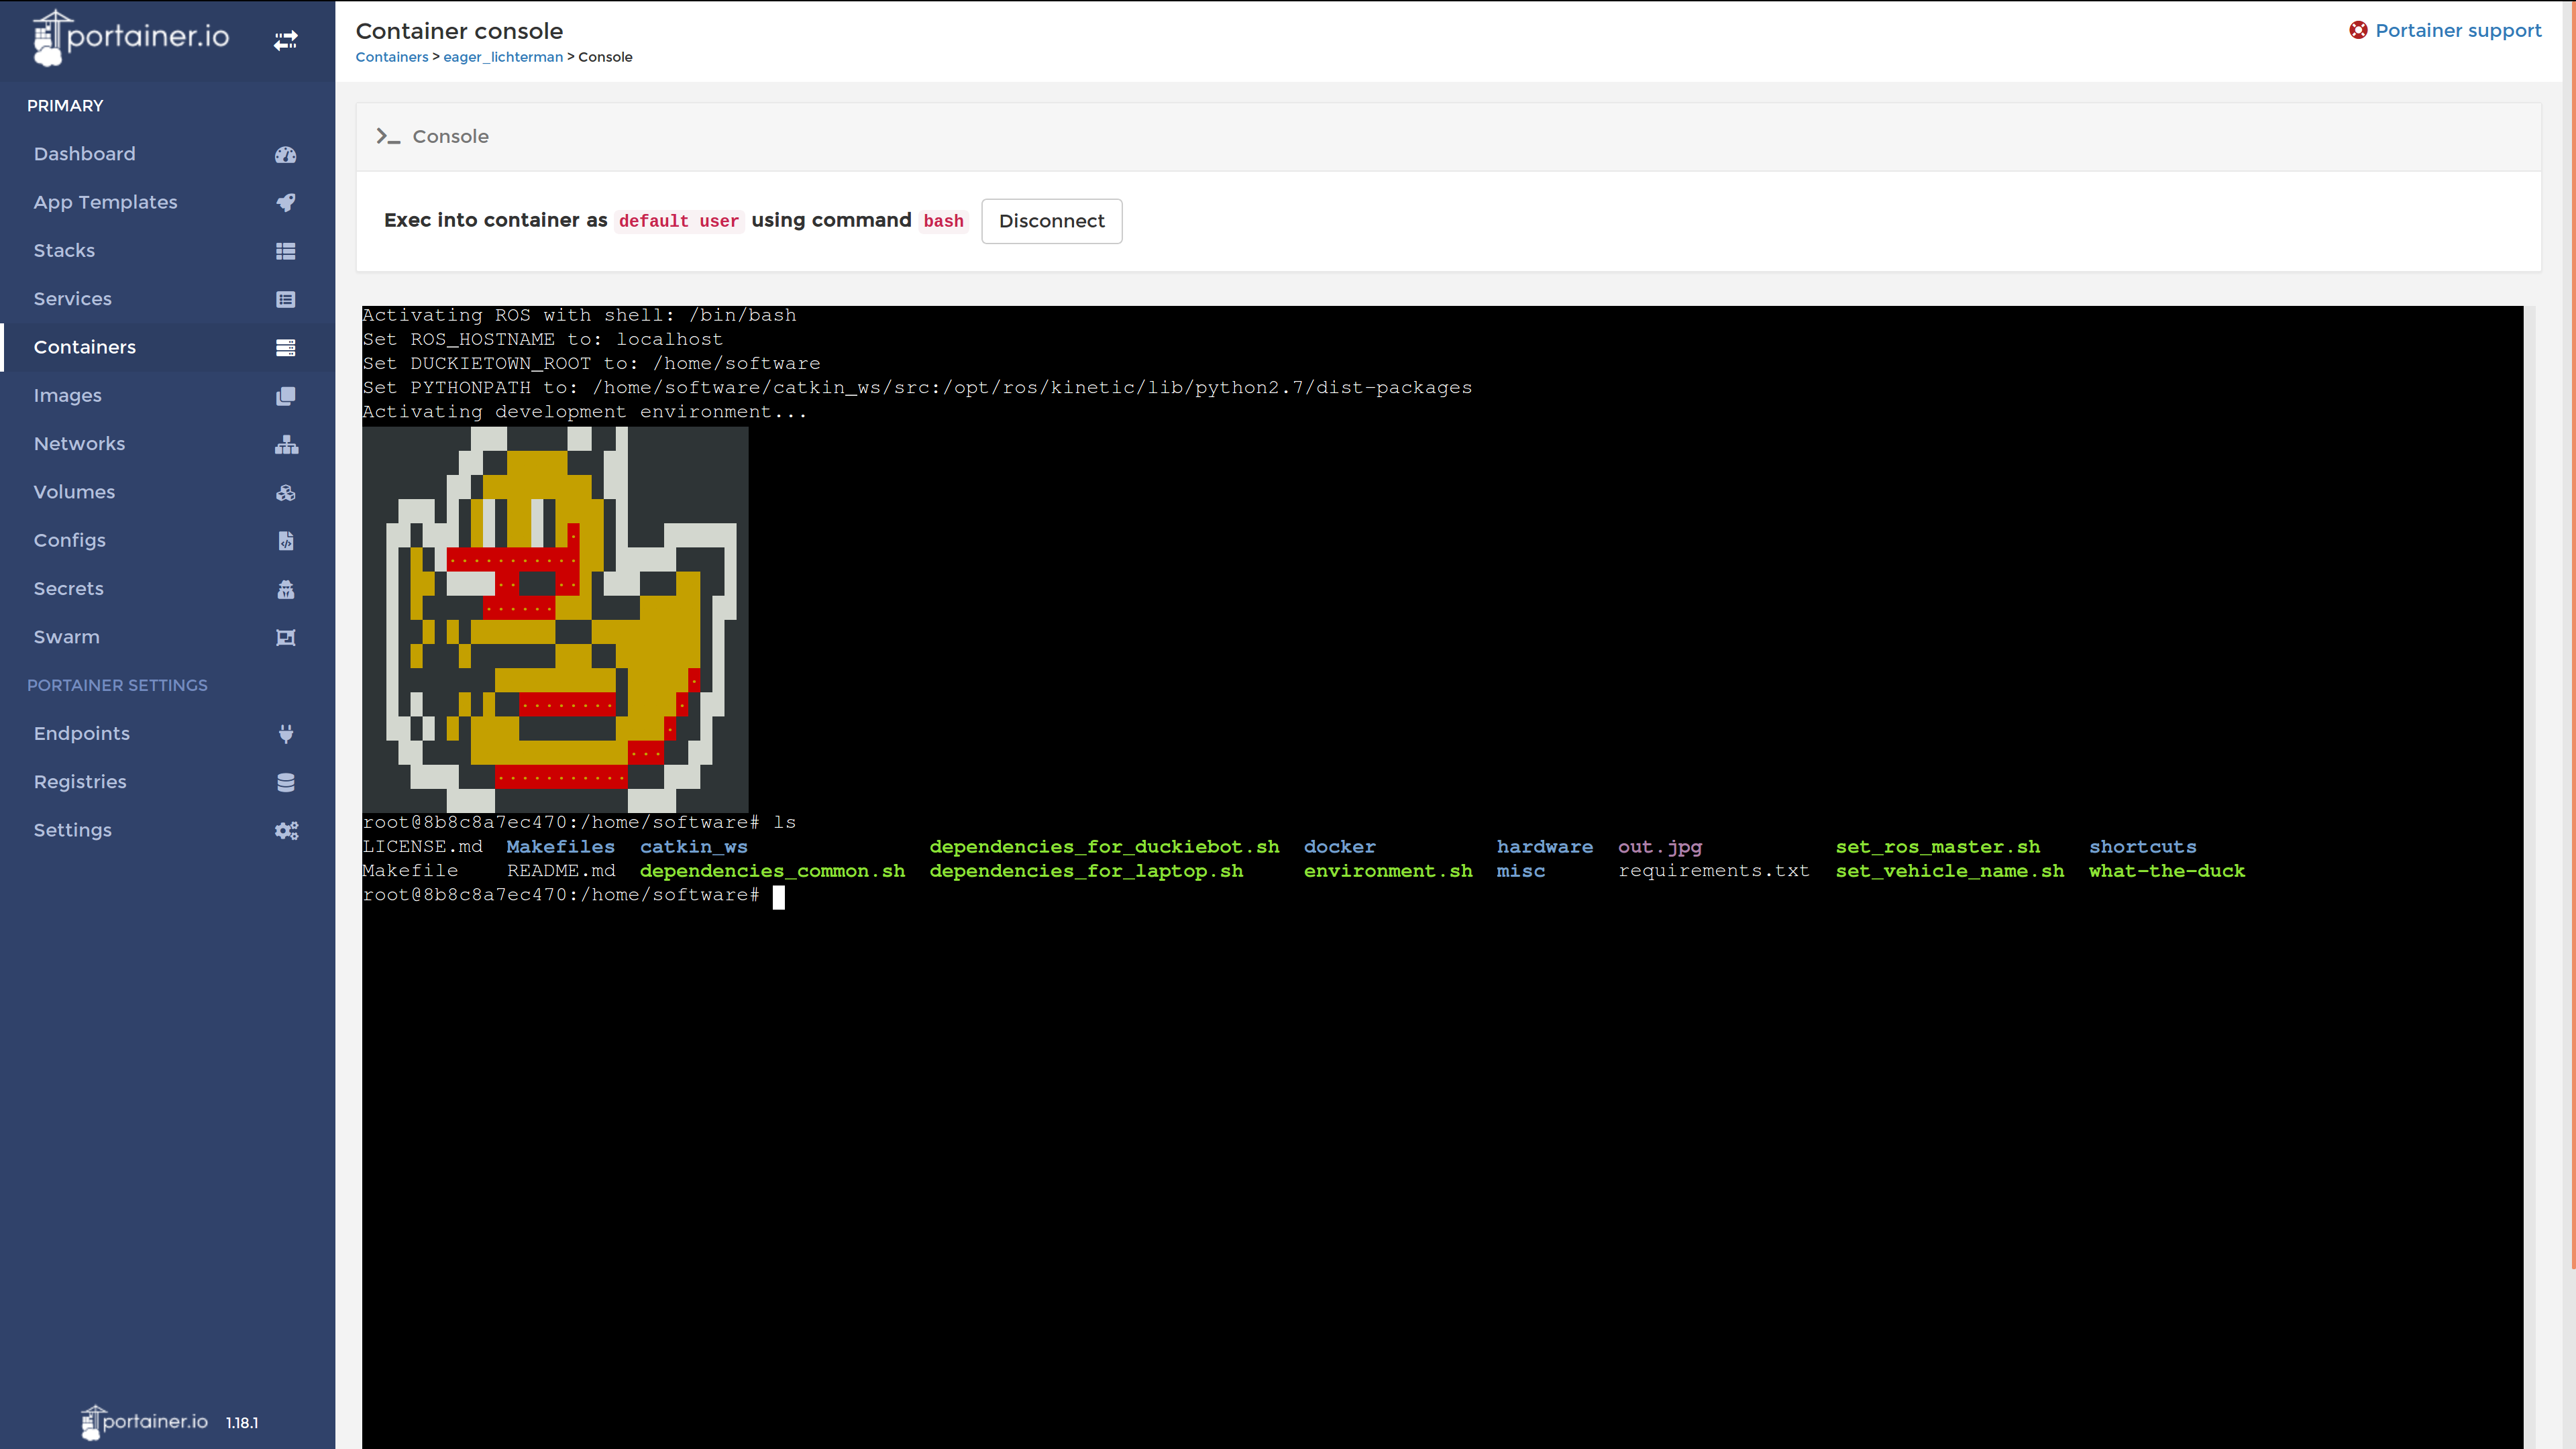
\includegraphics[width=0.80\textwidth]{portainer_screenshot.png}
    \caption{Browser interface for individual Duckiebots. It is provided by Portainer, a wrapper for the Docker CLI which has support for container management and terminal emulation.}
\end{figure}

\subsection{Testing ROS}

To verify Docker is working properly, launch a remote container, interactively, like so:

\begin{pclisting}
~$ docker -H DUCKIEBOT_NAME run -it \
   --name test \
   --privileged \
   --net host \
   duckietown/rpi-ros-kinetic-base:master18
\end{pclisting}

The \inline{-H} flag indicates a remote Docker host on the local area network where the Docker command should be executed. For the \inline{DUCKIEBOT_NAME} address it to work, mDNS must be configured properly in the network settings beforehand, otherwise an IP address is required.

\subsection{Build and deployment}

Docker images can be cross-compiled by enclosing the ARM-specific portion of the \inline{Dockerfile} with the \inline{RUN [ "cross-build-start" ]} and \inline{RUN [ "cross-build-end" ]} instructions. The following command can be used for deployment:

\begin{pclisting}
~$ docker save TAG_NAME | ssh -C duckie@DUCKIEBOT_NAME docker load
\end{pclisting}

Alternately, it is possible to build directly on ARM devices by creating a file named \inline{Dockerfile.arm}, adding a base image and build instructions, then running the command:

\begin{rpilisting}
~$ docker build --file=[FILE PATH]/Dockerfile.arm --tag [TAG NAME] .
\end{rpilisting}

\subsection{Multi-architecture support}

As of Docker version 18.09.6, ARM-specific \inline{Dockerfile}s will not build on x86 machines\footnote{With the exception of the Mac OS Docker client, which offers multi-architecture support. Further details on multiarch support can be found here: \url{https://docs.docker.com/docker-for-mac/multi-arch/}. Later versions of Docker for Mac OS and Windows provide native ARM emulation, which was recently announced at the following URL: \url{https://engineering.docker.com/2019/04/multi-arch-images/}}, and attempting to build one will produce the following error when running \inline{docker build}:

\begin{pclisting}
standard_init_linux.go:175: exec user process caused "exec format error"
\end{pclisting}

In order to circumvent this restriction, ARM-specific \inline{Dockerfile}s can ported to run on x86 by using the \inline{RUN [ "cross-build-start" ]} and \inline{RUN [ "cross-build-end" ]} directives, after the \inline{FROM} and before the \inline{CMD} instructions.

All Duckietown Docker images contain an emulator called QEMU - this allows us to run ARM images on x86 directly. To run a pure compute ROS node (i.e.\ one that does not require any camera or motor access) on an x86 platform, developers must supply a custom entrypoint to Docker when running the image using the entrypoint flag as follows:

\begin{pclisting}
~$ docker run ... --entrypoint=qemu3-arm-static IMAGE [RUN_COMMAND]
\end{pclisting}

Here, \inline{RUN_COMMAND} may be a shell such as \inline{/bin/bash} or another command such as \inline{/bin/bash -c "roscore"}. The \inline{qemu3-arm-static} entrypoint is an emulator provided by the base image, \inline{duckietown/rpi-ros-kinetic-base}.

\subsection{Running Simple HTTP File Server}

All persistent data is stored in \inline{/data}. To serve this directory, a web server is provided:

\begin{pclisting}
~$ docker -H DUCKEBOT_NAME run -d \
   --name file-server \
   -v /data:/data \
   -p 8082:8082 \
   duckietown/rpi-simple-server:master18
\end{pclisting}

To access this directory, visit the following URL: \url{http://DUCKIEBOT_NAME:8082/}

\subsection{Testing the camera}

The following image can be used to test the camera is working properly:

\begin{pclisting}
~$ docker -H DUCKIEBOT_NAME run -d \
   --privileged \
   --name picam \
   -v /data:/data \
   -p 8081:8081 \
   duckietown/rpi-docker-python-picamera:master18
\end{pclisting}

By default, images will be hosted at: \url{http://DUCKIEBOT_NAME:8081/image.jpg}

\begin{dtslisting}
dt> duckiebot demo --demo_name camera --duckiebot_name DUCKIEBOT_NAME
\end{dtslisting}

\subsection{Graphical User Interface Tools}

To use GUI tools, first allow incoming X connections. On Linux hosts, this can be done by running \inline{xhost +} from outside Docker.\footnote{See \url{http://wiki.ros.org/docker/Tutorials/GUI#The_safer_way} for a more secure alternative.} A container with common ROS GUI plugins can be started with following command:

\begin{pclisting}
~$ docker run -it --rm \
   --name rosgui \
   --net host \
   --env ROS_MASTER_URI=http://DUCKIEBOT_IP:11311 \
   --env ROS_IP=LAPTOP_IP \
   --env="DISPLAY" \
   --env="QT_X11_NO_MITSHM=1" \
   --volume="/tmp/.X11-unix:/tmp/.X11-unix:rw" \
   duckietown/rpi-gui-tools
\end{pclisting}

\begin{dtslisting}
dt> start_gui_tools DUCKIEBOT_NAME rqt_image_view
\end{dtslisting}

The above command opens a ROS shell that will connect to the \inline{DUCKIEBOT}'s ROS master node. To test the ROS connection works, run \inline{roswtf}.

\subsection{Remote control}

The following container launches the joystick demo (USB joystick must be connected):

\begin{pclisting}
~$ docker -H DUCKIEBOT_NAME run -d \
   --name joystick-demo \
   --privileged \
   -v /data:/data \
   --net host \
   duckietown/rpi-duckiebot-joystick-demo:master18
\end{pclisting}

\begin{dtslisting}
dt> duckiebot demo --demo_name joystick --duckiebot_name DUCKIEBOT_NAME
\end{dtslisting}

\begin{dtslisting}
dt> duckiebot keyboard_control DUCKIEBOT_NAME
\end{dtslisting}

\subsection{Calibration}

The following container will launch the extrinsic calibration procedure:

\begin{pclisting}
~$ docker -H DUCKIEBOT_NAME run -it \
   --name calibration \
   --privileged \
   -v /data:/data \
   --net host \
   duckietown/rpi-duckiebot-calibration:master18
\end{pclisting}

Passing \inline{-v /data:/data} is necessary so that all calibration settings will be preserved. Place the Duckiebot on the calibration pattern and follow the instructions provided.

\begin{dtslisting}
dt> duckiebot calibrate_extrinsics DUCKIEBOT_NAME
\end{dtslisting}

\begin{dtslisting}
dt> duckiebot calibrate_intrinsics DUCKIEBOT_NAME
\end{dtslisting}


\begin{dtslisting}
dt> duckiebot demo --demo_name base --duckiebot_name NAME
\end{dtslisting}

\begin{pclisting}
~$ rosservice call /DUCKIEBOT_NAME/inverse_kinematics_node/set_trim --TRIM
\end{pclisting}

\subsection{Lane Following Demo}

Once calibrated, the Lane Following Demo can be launched as follows:

\begin{pclisting}
~$ docker -H DUCKIEBOT_NAME run -it \
   --name lanefollowing-demo \
   --privileged \
   -v /data:/data \
   --net host \
   duckietown/rpi-duckiebot-lanefollowing-demo:master18
\end{pclisting}

\begin{dtslisting}
dt> duckiebot demo --demo_name lane_following --duckiebot_name DUCKIEBOT_NAME
\end{dtslisting}

\section{Retrospective}

One problem encountered during the development of Duckietown's Docker infrastructure was the matter of whether to package source code directly inside the container, or to store the sources externally (e.g. as described in \autoref{subsec:volume_sharing}). If stored externally, a developer can share the sources in a shared volume and build the artifacts on container startup. Both approaches ensure reproducible build dependencies, but including the the source code makes build artifacts are standalone decipherable.

Initially, we made the explicit decision to ship user source code directly inside the image. As a consequence, any changes to the source code would trigger a subsequent rebuild, tying the sources and Docker image together. The motivation for including sources enables easier troubleshooting and diagnostics, but doing so adds some friction during development, which has caused users to struggle with environment setup and Docker configuration issues.

\begin{figure}\label{fig:early_prototype}
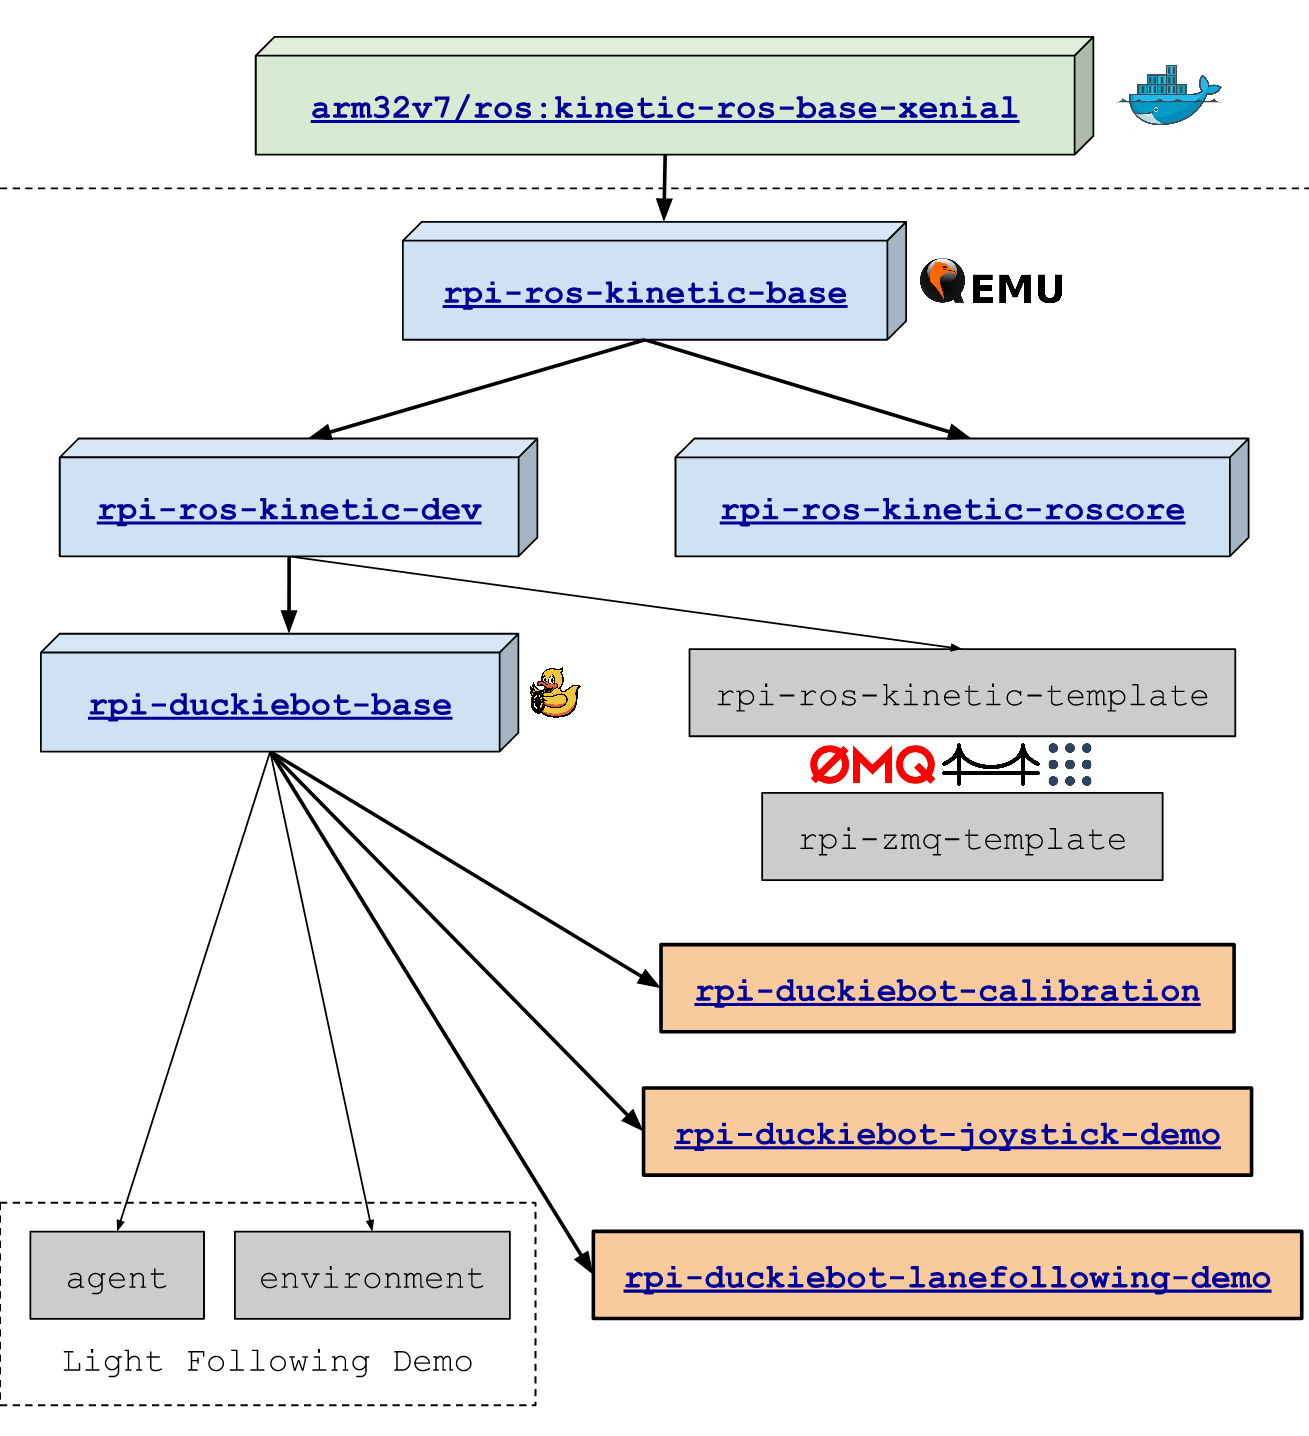
\includegraphics[width=0.80\textwidth]{image_provenance.png}
\caption{Early prototype of the Docker image hierarchy. Chaining unversioned autobuilds without disciplined unit testing tends to produce an undesirable domino effect, where breaking changes are allowed to propagate downstream, resulting in a cascade of silent failures.}
\end{figure}

The root cause of this friction was a product of imprecise versioning and over-automation. As version tags were initially omitted, all images were built and pulled from latest commit on the mainline development branch. The auto-build feature of the CI server caused upstream changes to cascade to downstream images. The short term solution was to disable auto-building and push manually, however fixing it required rethinking the role of Docker builds in the CI toolchain.

\begin{figure}\label{fig:early_prototype}

\includegraphics[width=0.40\textwidth]{aido_logo.png}
\caption{The AI Driving Olympics, a primary use case for the system described above.}
\end{figure}

One of the primary use cases for the container infrastructure is a biannual robotics competition called the AI Driving Olympics~\citep{aido2018}. We discovered a more stable solution is to store all sources on the local development environment and rebuild the image only when its upstream dependencies change. A Docker image, paired with a Git repository and a commit message defines an AIDO submission. The image only contains its compiled upstream dependencies, and the source code is paired at runtime.

\rare{\chapter{Case study: application for autonomous robotics}\label{ch:case-study}}

\setlength{\epigraphwidth}{0.80\textwidth}
\epigraph{``Thus, I came to the conclusion that the designer of a new system must not only be the implementor and the first large-scale user; the designer should also write the first user manual. The separation of any of these four components would have hurt TeX significantly. If I had not participated fully in all these activities, literally hundreds of improvements would never have been made, because I would never have thought of them or perceived why they were important.''}{\begin{flushright}-- Donald E.~\citet{knutherrors}, \textit{The errors of TeX}\end{flushright}}

As a case study, we have implemented a mobile application using ROS, Docker, and Android, using the proposed toolchain.

\section{Design}

Designed with Hatchery.

\section{Implementation}

Implementation includes Kotlin$\nabla$

\section{Testing and validation}

Verified using property-based testing.

\section{Containerization}

Deployed and CI-tested using Docker.

\rare{\chapter{Conclusion}\label{ch:conclusion}}

\section{Future work}

\subsection{Requirements Engineering}

Often it is not possible, or desirable to summarize the performance of a complex system using a single variable. In multi-objective optimization, we have the notion of pareto-efficiency...

Traditional software engineering has followed a rigorous process model and testing methodology. This model has guided the development of traditional software engineering, intelligent systems will require a re-imagining of these ideas to build systems that adapt to their environment during operation. Intelligent systems are designed with objective functions, which are typically one- or low-dimensional metrics for evaluating the performance of the system. Most often, these take the form of a single criteria, such as an \textit{error} or \textit{loss} which can represent descriptive phenomena such as latency, safety, energy efficiency or any number of objective measures.

For example, in the design of a web based advertisement recommendation system, we can optimize for various objectives such as click rate, engagement, sales conversion. So long as we can measure these parameters, with today's powerful function approximators, we can optimize for any single criterion or combination thereof. Much of the work involved in machine learning is to find representations which are amenable to learning, and preventing unintended consequences. For example, by optimizing for click rate, we create an artificial market for click bots. Similarly, in self driving cars, we often want to optimize for passenger safety. However by doing so naively, we create a vehicle that never moves, or always yields to nearby vehicles.

When building an intelligent system developers must first ask, ``What are the requirements of the system?'' This question is often the most troublesome part, because the requirements must not be fuzzy specifications like traditional software engineering, but precise, programmable directives. ``The system must be fast,'' is not sufficiently precise. These kinds of requirements must be translated into statistical loss functions, so intelligent systems engineers must be very precise when specifying requirements. If we simply say, ``The system must produce a valid response as quickly as possible, in less than 100ms,'' is better, but leaves open the possibility of returning an empty response.

In traditional software engineering, it is reasonable to assume the people who are implementing a system have some implicit knowledge and are generally well-intentioned human beings working towards the same goal. When building an intelligent system, a more reasonable assumption is that the entity implementing our requirements is a naive but powerful genie, and possibly an adversarial one. When given an optimization metric, it will take every available shortcut to meet that metric. If we are not careful about requirements engineering, this entity can produce a system that does not work, or has unintended consequences.

In the strictest sense, designing a good set of requirements is indistinguishable from implementing the system. With the right language abstractions (e.g.\ declarative programming), requirements and implementation can be the same thing. These ideas have been explored in recent decades with languages like SQL and Prolog. While these are toy systems, neural networks can express much larger classes of functions than traditional software engineering.

\subsection{Continuous Delivery and Continual Learning}

An ongoing trend in modern software and systems engineering is the transition away from long development cycles towards continuous integration and deployment. Development teams across the industry are encouraged to iterate in a series of short sprints between feature development and deployment. In some cases, software is shipped to users on a nightly basis, with automated testing and deployment. Similarly, intelligent systems have a need to continuously adapt to their environment, and will change their behavior on an even shorter basis.

%Incremental updates will grow increasingly smaller, until the program starts to alter itself after every input it processes.

%We need tools to more effectively harness the stochasticity of these learning systems.

%\subsection{Developers, Operations, and the DevOps toolchain}
%
%Software engineers have begun to realize the value of bespoke tools that facilitate the process of shipping software, in addition to the software itself.
%
%Teams building software are cybernetic systems, and require meta-programs for building code and organizational processes which enable them to ship code more efficiently.

\bibliography{thesis}
\bibliographystyle{plainnat}
\end{document}
